% Chapter 1

\chapter{Introducción general} % Main chapter title

\label{Chapter1} % For referencing the chapter elsewhere, use \ref{Chapter1} 
\label{IntroGeneral}

En este capítulo se presenta el contexto general y la motivación del trabajo realizado.
A su vez se realiza un análisis del estado del arte relacionado con las tecnologías que se utilizaron
y se concretan los objetivos y el alcance definidos durante su realización.
%----------------------------------------------------------------------------------------

% Define some commands to keep the formatting separated from the content 
\newcommand{\keyword}[1]{\textbf{#1}}
\newcommand{\tabhead}[1]{\textbf{#1}}
\newcommand{\code}[1]{\texttt{#1}}
\newcommand{\file}[1]{\texttt{\bfseries#1}}
\newcommand{\option}[1]{\texttt{\itshape#1}}
\newcommand{\grados}{$^{\circ}$}

%----------------------------------------------------------------------------------------

%\section{Introducción}

%----------------------------------------------------------------------------------------
\section{Es desafío de la creación narrativa}

La narrativa es un género literario que relata un conjunto de sucesos
protagonizados por uno o más personajes y que son presentados a través de un narrador.
Se trata de una forma de expresión cultural fundamental, presente todas las culturas y épocas,
utilizado para entrener y transmitir conocimiento.
Una de sus características esenciales es la presencia de elementos ficticios, ya sea de manera parcial o total,
con la única excepción del subgénero de crónicas que se limita a relatar hechos reales.
La narrativa sigue siendo un elemento central de la cultura y está
presente en múltiples formatos como la literatura, el cine, la televisión y otros medios tanto físicos como digitales.

La inclusión de elementos ficticios en la narrativa es un proceso creativo
en el que el autor recurre a su imaginación para concebir componentes que, aunque inventados,
resulten verosímiles y significativos.
En este ejercicio mental intervienen múltiples factores, como la coherencia interna y la relación 
entre los distintos elementos que conforman la historia en el espacio y el tiempo.
Estas variables se vuelven especialmente complejas en narrativas con una alta carga ficticia
donde se inventan, además de los personajes y sucesos, contextos completos.
Aquí es donde cobra especial relevancia la construcción de mundos, un recurso narrativo fundamental que permite
al escritor diseñar entornos imaginarios detallados y capaces de sostener la lógica del relato.

El proceso de creación de mundos es tan complejo como la narrativa que busca sostentar y
la intención del autor de sumergir al lector dentro de la historia.
En la figura \ref{fig:worldBuildingElements} se presenta una lista amplia, aunque no completa,
de componentes fundamentales en la constrccuón de mundos 
y la manera en que estos se relacionan entre sí para dar cohesión al conjunto narrativo.

\begin{figure}[htbp]
	\centering
	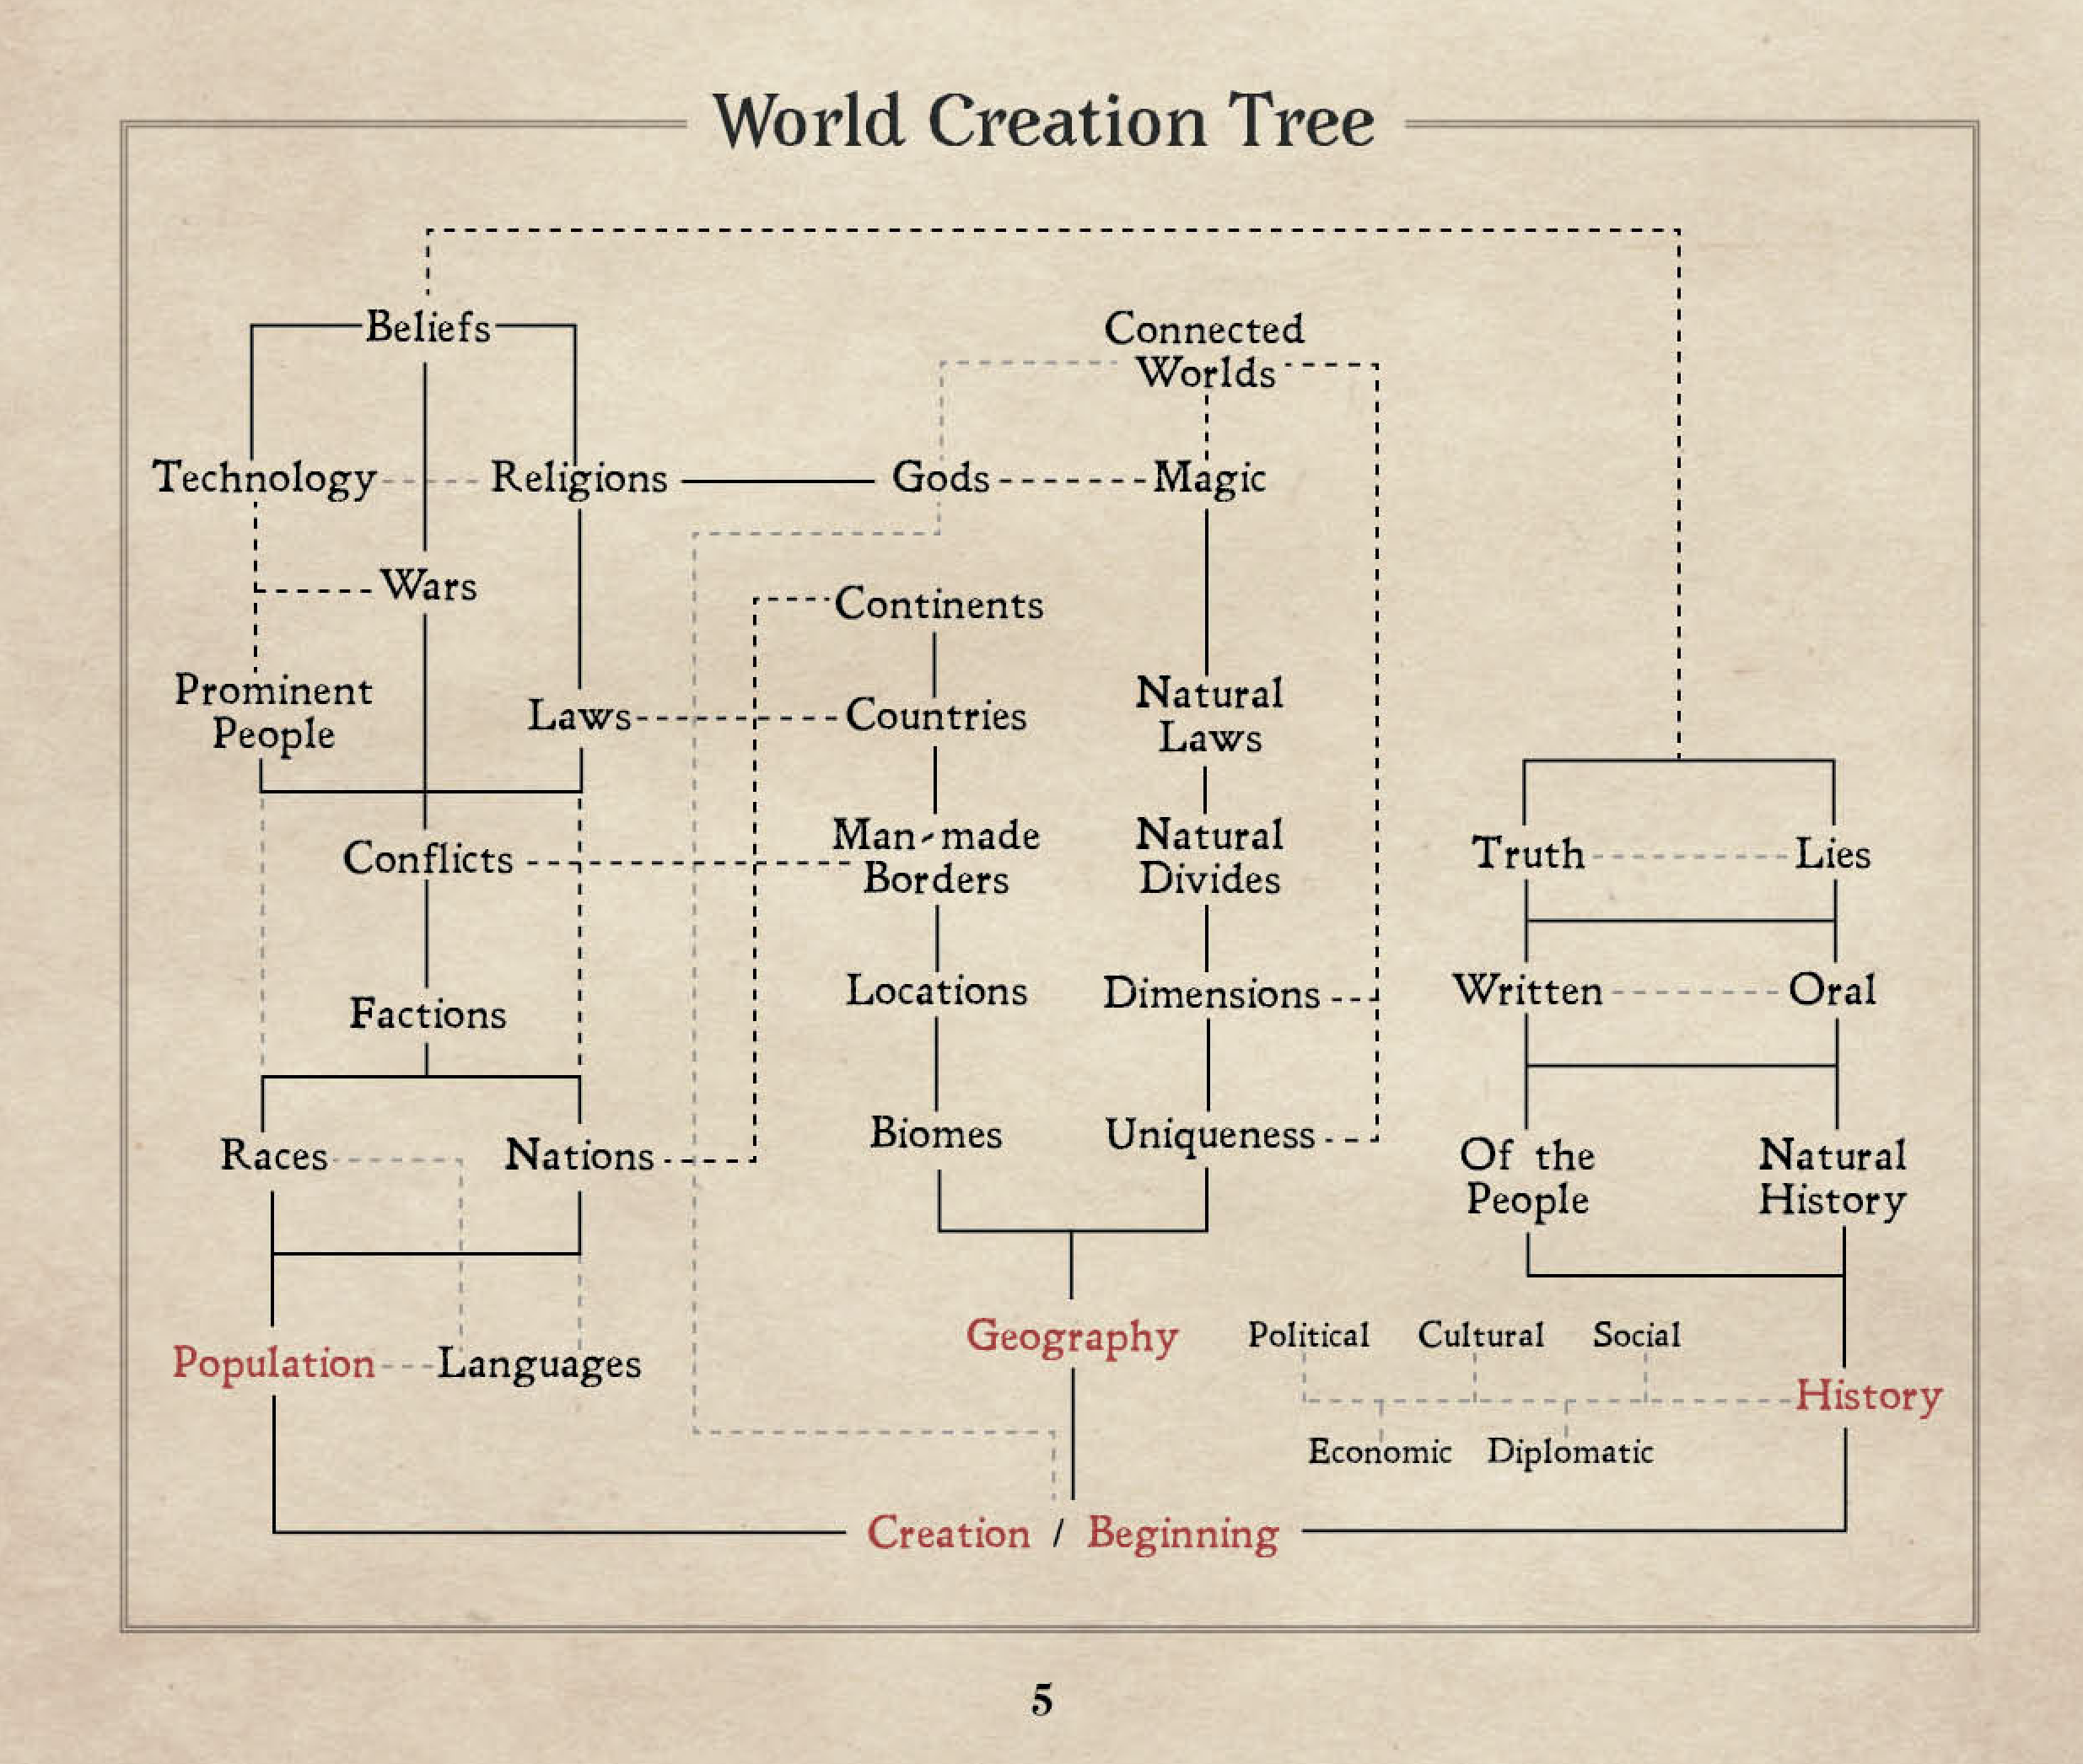
\includegraphics[width=0.9\textwidth]{./Figures/world-building-elements.png}
	\caption{Esquema de elementos habituales en la construcción de mundos.}
	\label{fig:worldBuildingElements}
\end{figure}

Históricamente los autores han recurrido a diversas herramientas para llevar a cabo la construcción de mundos,
tales como esquemas, mapas, cronologías, fichas de personajes y la creación de lenguas artificiales.
\footnote{Un ejemplo destacado es J.R.R. Tolkien, quien creó mapas, genealogías y lenguas para su obra
\textit{El Señor de los Anillos} \cite{tolkien_letters}.}
Todos estos elementos han sido producto del trabajo creativo del autor, apoyado tanto en su imaginación como en la
consulta de múltiples referencias.
Este proceso ha requerido una considerable inversión de tiempo y, en muchas ocasiones,
afectado por bloqueos creativos a la hora de articular y cohesionar todos los componentes ficticios de la narrativa.

En los últimos años la aparición de la inteligencia artificial generativa ha abierto nuevas posibilidades
dentro de los entornos creativos.
Aunque originalmente no fue concebida con fines narrativos, su capacidad para producir texto coherente
la convierte en una herramienta con un alto potencial para incorporarse en la construcción de mundos ficticios.
Sin pretender sutituir la creatividad del autor, estas tecnologías pueden ejercer un papel de apoyo
al facilitar el desarrollo de contenidos y aportar ideas que estimulen la creación literaria.

\section{Motivación}
El proyecto y consecuente trabajo se enfoca en la creación de entornos narrativos para juegos de rol 
y surgió de la Colaboración con la empresa Critical Match y su objetivo de ampliar las herramientas 
y servicios para sus usuarios de su apicación de móvil.
La aplicación permite la creación y búsqueda de salas de juego que se ajusten a las necesidades y preferencias de cada usuario.
En ese contexto, se busca mejorar la ambientación de las partidas proporcionando al autor de la narrativa a una serie de servicios
para complementar la construcción de mundo existente.

Estos servicios pretenden ofrecer una experiencia claramente diferenciada de las alternativas más populares en internet
\footnote{Algunos ejemplos son ChatGPT de OpenAI, Gemini de Google o LLaMA de Meta.}.
Para ello, se proporcionan a los usuarios el acceso a consultas especializadas que solo requieren el envío de un fichero
con la información narrativa, pudiendo combinarse adicionalmente con indicacions que pueden escribirse en un cuadro de texto.
Este enfoque no solo evita la incomodidad de interactuar con el modelo a través del navegador de internet del móvil,
sino que ofrece respuestas precisas a sus necesidades que requerirían interacciones complejas con las alternativas existentes.

Además, este desarrollo se relaciona de forma sinérgica con herramientas de creacion de mundos
\footnote{Por ejemplo, WorldAnvil, Obsidian Portal o Legend Keeper.}.
Mientras que estas plataformas proporcionan estructura y el marco para la creacion de mundos,
el trabajo ofrece la capacidad de generar dinamicamente contenido narrativo específico con la información ya existente.
De este modo los autores a traves de ambas herramientas pueden centrarse en la vision general y cohesion del mundo mientras que la inteligencia artificial 
los ayuda con ideas con las que expandir la ambientación, fomentando un proceso cíclico creativo.

%----------------------------------------------------------------------------------------

\section{Qué incluye esta plantilla}

\subsection{Carpetas}

Esta plantilla se distribuye como una único archivo .zip que se puede descomprimir en varios archivos y carpetas. Asimismo, se puede consultar el repositorio git para obtener la última versión de los archivos, \url{https://github.com/patriciobos/Plantilla-CESE.git}. Los nombres de las carpetas son, o pretender ser, auto-explicativos.

\keyword{Appendices} -- Esta es la carpeta donde se deben poner los apéndices. Cada apéndice debe ir en su propio archivo \file{.tex}. Se incluye un ejemplo y una plantilla en la carpeta.

\keyword{Chapters} -- Esta es la carpeta donde se deben poner los capítulos de la memoria. Cada capítulo debe ir un su propio archivo \file{.tex} por separado.  Se ofrece por defecto, la siguiente estructura de capítulos y se recomienda su utilización dentro de lo posible:

\begin{itemize}
\item Capítulo 1: Introducción general	
\item Capítulo 2: Introducción específica
\item Capítulo 3: Diseño e implementación
\item Capítulo 4: Ensayos y resultados
\item Capítulo 5: Conclusiones

\end{itemize}

Esta estructura de capítulos es la que se recomienda para las memorias de la especialización.

\keyword{Figures} -- Esta carpeta contiene todas las figuras de la memoria.  Estas son las versiones finales de las imágenes que van a ser incluidas en la memoria.  Pueden ser imágenes en formato \textit{raster}\footnote{\url{https://en.wikipedia.org/wiki/Raster_graphics}} como \file{.png}, \file{.jpg} o en formato vectoriales\footnote{\url{https://en.wikipedia.org/wiki/Vector_graphics}} como \file{.pdf}, \file{.ps}.  Se debe notar que utilizar imágenes vectoriales disminuye notablemente el peso del documento final y acelera el tiempo de compilación por lo que es recomendable su utilización siempre que sea posible.

\subsection{Archivos}

También están incluidos varios archivos, la mayoría de ellos son de texto plano y se puede ver su contenido en un editor de texto. Después de la compilación inicial, se verá que más archivos auxiliares son creados por \ LaTeX{} o BibTeX, pero son de uso interno y no es necesario hacer nada en particular con ellos.  Toda la información necesaria para compilar el documento se encuentra en los archivos \file{.tex}, \file{.bib}, \file{.cls} y en las imágenes de la carpeta Figures.

\keyword{referencias.bib} - este es un archivo importante que contiene toda la información de referencias bibliográficas que se utilizarán para las citas en la memoria en conjunto con BibTeX. Usted puede escribir las entradas bibliográficas en forma manual, aunque existen también programas de gestión de referencias que facilitan la creación y gestión de las referencias y permiten exportarlas en formato BibTeX.  También hay disponibles sitios web como \url{books.google.com} que permiten obtener toda la información necesaria para una cita en formato BibTeX. Ver sección \ref{sec:biblio}

\keyword{MastersDoctoralThesis.cls} -- este es un archivo importante. Es el archivos con la clase que le informa a \LaTeX{} cómo debe dar formato a la memoria. El usuario de la plantilla no debería necesitar modificar nada de este archivo.

\keyword{memoria.pdf} -- esta es su memoria con una tipografía bellamente compuesta (en formato de archivo PDF) creado por \LaTeX{}. Se distribuye con la plantilla y después de compilar por primera vez sin hacer ningún cambio se debería obtener una versión idéntica a este documento.

\keyword{memoria.tex} -- este es un archivo importante. Este es el archivo que tiene que compilar \LaTeX{} para producir la memoria como un archivo PDF. Contiene un marco de trabajo y estructuras que le indican a \LaTeX{} cómo diagramar la memoria.  Está altamente comentado para que se pueda entender qué es lo que realiza cada línea de código y por qué está incluida en ese lugar.  En este archivo se debe completar la información personalizada de las primeras sección según se indica en la sección \ref{sec:FillingFile}.

Archivos que \emph{no} forman parte de la distribución de la plantilla pero que son generados por \LaTeX{} como archivos auxiliares necesarios para la producción de la memoria.pdf son:

\keyword{memoria.aux} -- este es un archivo auxiliar generado por \LaTeX{}, si se borra \LaTeX{} simplemente lo regenera cuando se compila el archivo principal \file{memoria.tex}.

\keyword{memoria.bbl} -- este es un archivo auxiliar generado por BibTeX, si se borra BibTeX simplemente lo regenera cuando se compila el archivo principal \file{memoria.tex}. Mientras que el archivo \file{.bib} contiene todas las referencias que hay, este archivo \file{.bbl} contine sólo las referencias que han sido citadas y se utiliza para la construcción de la bibiografía.

\keyword{memoria.blg} -- este es un archivo auxiliar generado por BibTeX, si se borra BibTeX simplemente lo regenera cuando se compila el archivo principal \file{memoria.tex}.

\keyword{memoria.lof} -- este es un archivo auxiliar generado por \LaTeX{}, si se borra \LaTeX{} simplemente lo regenera cuando se compila el archivo principal \file{memoria.tex}.  Le indica a \LaTeX{} cómo construir la sección \emph{Lista de Figuras}.
 
\keyword{memoria.log} --  este es un archivo auxiliar generado por \LaTeX{}, si se borra \LaTeX{} simplemente lo regenera cuando se compila el archivo principal \file{memoria.tex}. Contiene mensajes de \LaTeX{}. Si se reciben errores o advertencias durante la compilación, se guardan en este archivo \file{.log}.

\keyword{memoria.lot} -- este es un archivo auxiliar generado por \LaTeX{}, si se borra \LaTeX{} simplemente lo regenera cuando se compila el archivo principal \file{memoria.tex}.  Le indica a \LaTeX{} cómo construir la sección \emph{Lista de Tablas}.

\keyword{memoria.out} -- este es un archivo auxiliar generado por \LaTeX{}, si se borra \LaTeX{} simplemente lo regenera cuando se compila el archivo principal \file{memoria.tex}.

De esta larga lista de archivos, sólo aquellos con la extensión \file{.bib}, \file{.cls} y \file{.tex} son importantes.  Los otros archivos auxiliares pueden ser ignorados o borrados ya que \LaTeX{} y BibTeX los regenerarán durante la compilación.

%----------------------------------------------------------------------------------------

\section{Entorno de trabajo}

Ante de comenzar a editar la plantilla debemos tener un editor \LaTeX{} instalado en nuestra computadora.  En forma análoga a lo que sucede en lenguaje C, que se puede crear y editar código con casi cualquier editor, existen ciertos entornos de trabajo que nos pueden simplificar mucho la tarea.  En este sentido, se recomienda, sobre todo para los principiantes en \LaTeX{} la utilización de TexMaker, un programa gratuito y multi-plantaforma que está disponible tanto para windows como para sistemas GNU/linux.

La versión más reciente de TexMaker es la 4.5 y se puede descargar del siguiente link: \url{http://www.xm1math.net/texmaker/download.html}. Se puede consultar el manual de usuario en el siguiente link: \url{http://www.xm1math.net/texmaker/doc.html}.
 

\subsection{Paquetes adicionales}

Si bien durante el proceso de instalación de TexMaker, o cualquier otro editor que se haya elegido, se instalarán en el sistema los paquetes básicos necesarios para trabajar con \LaTeX{}, la plantilla de los trabajos de Especialización y Maestría requieren de paquete adicionales.

Se indican a continuación los comandos que se deben introducir en la consola de Ubuntu (ctrl + alt + t) para instalarlos:

\begin{lstlisting}[language=bash]
  $ sudo apt install texlive-lang-spanish texlive-science 
  $ sudo apt install texlive-bibtex-extra biber
  $ sudo apt install texlive texlive-fonts-recommended
  $ sudo apt install texlive-latex-extra
\end{lstlisting}


\subsection{Configurando TexMaker}
\label{subsec:configurando}



Una vez instalado el programa y los paquetes adicionales se debe abrir el archivo memoria.tex con el editor para ver una pantalla similar a la que se puede apreciar en la figura \ref{fig:texmaker}. 
Una vez instalado el programa y los paquetes adicionales se debe abrir el archivo memoria.tex con el editor para ver una pantalla similar a la que se puede apreciar en la figura \ref{fig:texmaker}. 
Una vez instalado el programa y los paquetes adicionales se debe abrir el archivo memoria.tex con el editor para ver una pantalla similar a la que se puede apreciar en la figura \ref{fig:texmaker}. 
Una vez instalado el programa y los paquetes adicionales se debe abrir el archivo memoria.tex con el editor para ver una pantalla similar a la que se puede apreciar en la figura \ref{fig:texmaker}. 

\vspace{1cm}

\begin{figure}[htbp]
	\centering
	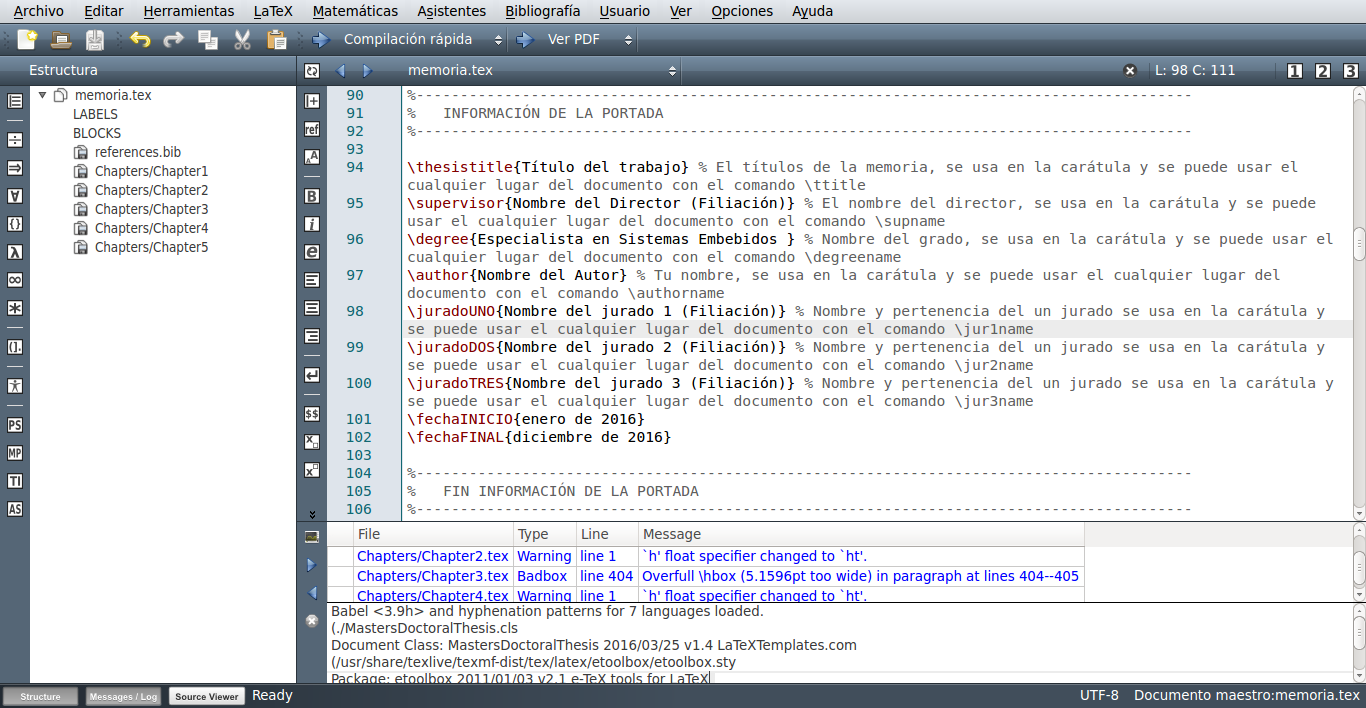
\includegraphics[width=.5\textwidth]{./Figures/texmaker.png}
	\caption{Entorno de trabajo de texMaker.}
	\label{fig:texmaker}
\end{figure}

\vspace{1cm}

Notar que existe una vista llamada Estructura a la izquierda de la interfaz que nos permite abrir desde dentro del programa los archivos individuales de los capítulos.  A la derecha se encuentra una vista con el archivo propiamente dicho para su edición. Hacia la parte inferior se encuentra una vista del log con información de los resultados de la compilación.  En esta última vista pueden aparecen advertencias o \textit{warning}, que normalmente pueden ser ignorados, y los errores que se indican en color rojo y deben resolverse para que se genere el PDF de salida.

Recordar que el archivo que se debe compilar con PDFLaTeX es \file{memoria.tex}, si se tratara de compilar alguno de los capítulos saldría un error.  Para salvar la molestia de tener que cambiar de archivo para compilar cada vez que se realice una modificación en un capítulo, se puede definir el archivo \file{memoria.tex} como ``documento maestro'' yendo al menú opciones -> ``definir documento actual como documento maestro'', lo que permite compilar con PDFLaTeX memoria.tex directamente desde cualquier archivo que se esté modificando . Se muestra esta opción en la figura \ref{fig:docMaestro}.

\begin{figure}[h]
	\centering
	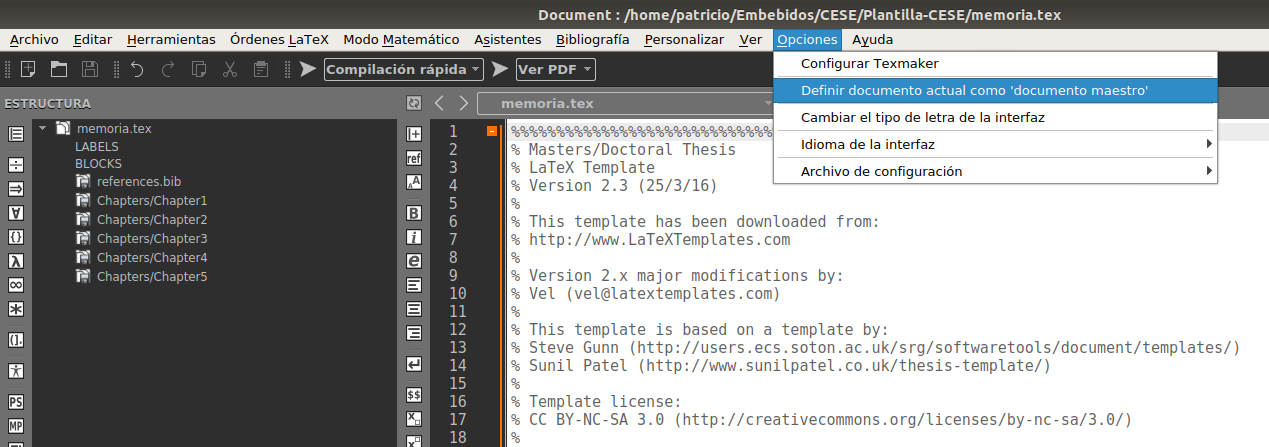
\includegraphics[width=\textwidth]{./Figures/docMaestro.png}
	\caption{Definir memoria.tex como documento maestro.}
	\label{fig:docMaestro}
\end{figure}

En el menú herramientas se encuentran las opciones de compilación.  Para producir un archivo PDF a partir de un archivo .tex se debe ejecutar PDFLaTeX (el shortcut es F6). Para incorporar nueva bibliografía se debe utilizar la opción BibTeX del mismo menú herramientas (el shortcut es F11).

Notar que para actualizar las tablas de contenidos se debe ejecutar PDFLaTeX dos veces.  Esto se debe a que es necesario actualizar algunos archivos auxiliares antes de obtener el resultado final.  En forma similar, para actualizar las referencias bibliográficas se debe ejecutar primero PDFLaTeX, después BibTeX y finalmente PDFLaTeX dos veces por idénticos motivos.

\section{Personalizando la plantilla, el archivo \file{memoria.tex}}
\label{sec:FillingFile}

Para personalizar la plantilla se debe incorporar la información propia en los distintos archivos \file{.tex}. 

Primero abrir \file{memoria.tex} con TexMaker (o el editor de su preferencia). Se debe ubicar dentro del archivo el bloque de código titulado \emph{INFORMACIÓN DE LA PORTADA} donde se deben incorporar los primeros datos personales con los que se construirá automáticamente la portada.


%----------------------------------------------------------------------------------------

\section{El código del archivo \file{memoria.tex} explicado}

El archivo \file{memoria.tex} contiene la estructura del documento y es el archivo de mayor jerarquía de la memoria.  Podría ser equiparable a la función \emph{main()} de un programa en C, o mejor dicho al archivo fuente .c donde se encuentra definida la función main().

La estructura básica de cualquier documento de \LaTeX{} comienza con la definición de clase del documento, es seguida por un preámbulo donde se pueden agregar funcionalidades con el uso de \texttt{paquetes} (equiparables a bibliotecas de C), y finalmente, termina con el cuerpo del documento, donde irá el contenido de la memoria.

\lstset{%
  basicstyle=\small\ttfamily,
  language=[LaTeX]{TeX}
}

\begin{lstlisting}
\documentclass{article}  <- Definicion de clase
\usepackage{listings}	 <- Preambulo

\begin{document}	 <- Comienzo del contenido propio 
	Hello world!
\end{document}
\end{lstlisting}


El archivo \file{memoria.tex} se encuentra densamente comentado para explicar qué páginas, secciones y elementos de formato está creando el código \LaTeX{} en cada línea. El código está dividido en bloques con nombres en mayúsculas para que resulte evidente qué es lo que hace esa porción de código en particular. Inicialmente puede parecer que hay mucho código \LaTeX{}, pero es principalmente código para dar formato a la memoria por lo que no requiere intervención del usuario de la plantilla.  Sí se deben personalizar con su información los bloques indicados como:

\begin{itemize}
	\item Informacion de la memoria
	\item Resumen
	\item Agradecimientos
	\item Dedicatoria
\end{itemize}

El índice de contenidos, las listas de figura de tablas se generan en forma automática y no requieren intervención ni edición manual por parte del usuario de la plantilla. 

En la parte final del documento se encuentran los capítulos y los apéndices.  Por defecto se incluyen los 5 capítulos propuestos que se encuentran en la carpeta /Chapters. Cada capítulo se debe escribir en un archivo .tex separado y se debe poner en la carpeta \emph{Chapters} con el nombre \file{Chapter1}, \file{Chapter2}, etc\ldots El código para incluir capítulos desde archivos externos se muestra a continuación.

\begin{verbatim}
	% Chapter 1

\chapter{Introducción general} % Main chapter title

\label{Chapter1} % For referencing the chapter elsewhere, use \ref{Chapter1} 
\label{IntroGeneral}

Todos los capítulos deben comenzar con un breve párrafo introductorio que indique cuál es el contenido que se encontrará al leerlo.  La redacción sobre el contenido de la memoria debe hacerse en presente y todo lo referido al proyecto en pasado, siempre de modo impersonal.

%----------------------------------------------------------------------------------------

% Define some commands to keep the formatting separated from the content 
\newcommand{\keyword}[1]{\textbf{#1}}
\newcommand{\tabhead}[1]{\textbf{#1}}
\newcommand{\code}[1]{\texttt{#1}}
\newcommand{\file}[1]{\texttt{\bfseries#1}}
\newcommand{\option}[1]{\texttt{\itshape#1}}
\newcommand{\grados}{$^{\circ}$}

%----------------------------------------------------------------------------------------

%\section{Introducción}

%----------------------------------------------------------------------------------------
\section{Aprendiendo \LaTeX{}}

\LaTeX{} no es \textsc{WYSIWYG} (What You See is What You Get), a diferencia de los procesadores de texto como Microsoft Word o Pages de Apple o incluso LibreOffice en el mundo open-source. En lugar de ello, un documento escrito para \LaTeX{} es en realidad un archivo de texto simple o llano que \emph{no contiene formato} . Nosotros le decimos a \LaTeX{} cómo deseamos que se aplique el formato en el documento final escribiendo comandos simples entre el texto, por ejemplo, si quiero usar texto en itálicas para dar énfasis, escribo \verb|\it{texto}| y pongo el texto que quiero en itálicas entre medio de las llaves. Esto significa que \LaTeX{} es un lenguaje del tipo \enquote{mark-up}, muy parecido a HTML.

\subsection{Una introducción (no tan corta) a \LaTeX{}}

Si sos nuevo en \LaTeX{}, hay un muy buen libro electrónico - disponible gratuitamente en Internet como un archivo PDF - llamado, \enquote{A (not so short) Introduction to \LaTeX{}}. El título del libro es generalmente acortado a simplemente \emph{lshort}. Puede descargar la versión más reciente en inglés (ya que se actualiza de vez en cuando) desde aquí:
\url{http://www.ctan.org/tex-archive/info/lshort/english/lshort.pdf}

Se puede encontrar la versión en español en la lista en esta página: \url{http://www.ctan.org/tex-archive/info/lshort/}

\subsubsection{Una subsubsección}

Acá tiene un ejemplo de una ``subsubsección'' que es el cuarto nivel de ordenamiento del texto, después de capítulo, sección y subsección.  Como se puede ver, las subsubsecciones no van numeradas en el cuerpo del documento ni en el índice.  El formato está definido por la plantilla y no debe ser modificado.

\subsection{Guía matemática rápida para \LaTeX{}}

Si estás escribiendo un documento con mucho contenido matemático, entonces es posible que desees leer el documento de la AMS (American Mathematical Society) llamado, \enquote{A Short Math Guide for \LaTeX{}}. Se puede encontrar en línea en el siguiente link: \url{http://www.ams.org/tex/amslatex.html} en la sección \enquote{Additional Documentation} hacia la parte inferior de la página.


%----------------------------------------------------------------------------------------

\section{Utilizando esta plantilla}

Si estás familiarizado con \LaTeX{}, entonces podés explorar la estructura de directorios de esta plantilla y proceder a personalizarla agregando tu información en el bloque \emph{INFORMACIÓN DE LA PORTADA} en el archivo \file{memoria.tex}.  

Se puede continuar luego modificando el resto de los archivos siguiendo los lineamientos que se describen en la sección \ref{sec:FillingFile} en la página \pageref{sec:FillingFile}.

Debés asegurarte de leer el capítulo \ref{Chapter2} acerca de las convenciones utilizadas para las Memoria de los Trabajos Finales de la \degreename.

Si sos nuevo en \LaTeX{}, se recomienda que continúes leyendo el documento ya que contiene información básica para aprovechar el potencial de esta herramienta.


%----------------------------------------------------------------------------------------

\section{Qué incluye esta plantilla}

\subsection{Carpetas}

Esta plantilla se distribuye como una único archivo .zip que se puede descomprimir en varios archivos y carpetas. Asimismo, se puede consultar el repositorio git para obtener la última versión de los archivos, \url{https://github.com/patriciobos/Plantilla-CESE.git}. Los nombres de las carpetas son, o pretender ser, auto-explicativos.

\keyword{Appendices} -- Esta es la carpeta donde se deben poner los apéndices. Cada apéndice debe ir en su propio archivo \file{.tex}. Se incluye un ejemplo y una plantilla en la carpeta.

\keyword{Chapters} -- Esta es la carpeta donde se deben poner los capítulos de la memoria. Cada capítulo debe ir un su propio archivo \file{.tex} por separado.  Se ofrece por defecto, la siguiente estructura de capítulos y se recomienda su utilización dentro de lo posible:

\begin{itemize}
\item Capítulo 1: Introducción general	
\item Capítulo 2: Introducción específica
\item Capítulo 3: Diseño e implementación
\item Capítulo 4: Ensayos y resultados
\item Capítulo 5: Conclusiones

\end{itemize}

Esta estructura de capítulos es la que se recomienda para las memorias de la especialización.

\keyword{Figures} -- Esta carpeta contiene todas las figuras de la memoria.  Estas son las versiones finales de las imágenes que van a ser incluidas en la memoria.  Pueden ser imágenes en formato \textit{raster}\footnote{\url{https://en.wikipedia.org/wiki/Raster_graphics}} como \file{.png}, \file{.jpg} o en formato vectoriales\footnote{\url{https://en.wikipedia.org/wiki/Vector_graphics}} como \file{.pdf}, \file{.ps}.  Se debe notar que utilizar imágenes vectoriales disminuye notablemente el peso del documento final y acelera el tiempo de compilación por lo que es recomendable su utilización siempre que sea posible.

\subsection{Archivos}

También están incluidos varios archivos, la mayoría de ellos son de texto plano y se puede ver su contenido en un editor de texto. Después de la compilación inicial, se verá que más archivos auxiliares son creados por \ LaTeX{} o BibTeX, pero son de uso interno y no es necesario hacer nada en particular con ellos.  Toda la información necesaria para compilar el documento se encuentra en los archivos \file{.tex}, \file{.bib}, \file{.cls} y en las imágenes de la carpeta Figures.

\keyword{referencias.bib} - este es un archivo importante que contiene toda la información de referencias bibliográficas que se utilizarán para las citas en la memoria en conjunto con BibTeX. Usted puede escribir las entradas bibliográficas en forma manual, aunque existen también programas de gestión de referencias que facilitan la creación y gestión de las referencias y permiten exportarlas en formato BibTeX.  También hay disponibles sitios web como \url{books.google.com} que permiten obtener toda la información necesaria para una cita en formato BibTeX. Ver sección \ref{sec:biblio}

\keyword{MastersDoctoralThesis.cls} -- este es un archivo importante. Es el archivos con la clase que le informa a \LaTeX{} cómo debe dar formato a la memoria. El usuario de la plantilla no debería necesitar modificar nada de este archivo.

\keyword{memoria.pdf} -- esta es su memoria con una tipografía bellamente compuesta (en formato de archivo PDF) creado por \LaTeX{}. Se distribuye con la plantilla y después de compilar por primera vez sin hacer ningún cambio se debería obtener una versión idéntica a este documento.

\keyword{memoria.tex} -- este es un archivo importante. Este es el archivo que tiene que compilar \LaTeX{} para producir la memoria como un archivo PDF. Contiene un marco de trabajo y estructuras que le indican a \LaTeX{} cómo diagramar la memoria.  Está altamente comentado para que se pueda entender qué es lo que realiza cada línea de código y por qué está incluida en ese lugar.  En este archivo se debe completar la información personalizada de las primeras sección según se indica en la sección \ref{sec:FillingFile}.

Archivos que \emph{no} forman parte de la distribución de la plantilla pero que son generados por \LaTeX{} como archivos auxiliares necesarios para la producción de la memoria.pdf son:

\keyword{memoria.aux} -- este es un archivo auxiliar generado por \LaTeX{}, si se borra \LaTeX{} simplemente lo regenera cuando se compila el archivo principal \file{memoria.tex}.

\keyword{memoria.bbl} -- este es un archivo auxiliar generado por BibTeX, si se borra BibTeX simplemente lo regenera cuando se compila el archivo principal \file{memoria.tex}. Mientras que el archivo \file{.bib} contiene todas las referencias que hay, este archivo \file{.bbl} contine sólo las referencias que han sido citadas y se utiliza para la construcción de la bibiografía.

\keyword{memoria.blg} -- este es un archivo auxiliar generado por BibTeX, si se borra BibTeX simplemente lo regenera cuando se compila el archivo principal \file{memoria.tex}.

\keyword{memoria.lof} -- este es un archivo auxiliar generado por \LaTeX{}, si se borra \LaTeX{} simplemente lo regenera cuando se compila el archivo principal \file{memoria.tex}.  Le indica a \LaTeX{} cómo construir la sección \emph{Lista de Figuras}.
 
\keyword{memoria.log} --  este es un archivo auxiliar generado por \LaTeX{}, si se borra \LaTeX{} simplemente lo regenera cuando se compila el archivo principal \file{memoria.tex}. Contiene mensajes de \LaTeX{}. Si se reciben errores o advertencias durante la compilación, se guardan en este archivo \file{.log}.

\keyword{memoria.lot} -- este es un archivo auxiliar generado por \LaTeX{}, si se borra \LaTeX{} simplemente lo regenera cuando se compila el archivo principal \file{memoria.tex}.  Le indica a \LaTeX{} cómo construir la sección \emph{Lista de Tablas}.

\keyword{memoria.out} -- este es un archivo auxiliar generado por \LaTeX{}, si se borra \LaTeX{} simplemente lo regenera cuando se compila el archivo principal \file{memoria.tex}.

De esta larga lista de archivos, sólo aquellos con la extensión \file{.bib}, \file{.cls} y \file{.tex} son importantes.  Los otros archivos auxiliares pueden ser ignorados o borrados ya que \LaTeX{} y BibTeX los regenerarán durante la compilación.

%----------------------------------------------------------------------------------------

\section{Entorno de trabajo}

Ante de comenzar a editar la plantilla debemos tener un editor \LaTeX{} instalado en nuestra computadora.  En forma análoga a lo que sucede en lenguaje C, que se puede crear y editar código con casi cualquier editor, existen ciertos entornos de trabajo que nos pueden simplificar mucho la tarea.  En este sentido, se recomienda, sobre todo para los principiantes en \LaTeX{} la utilización de TexMaker, un programa gratuito y multi-plantaforma que está disponible tanto para windows como para sistemas GNU/linux.

La versión más reciente de TexMaker es la 4.5 y se puede descargar del siguiente link: \url{http://www.xm1math.net/texmaker/download.html}. Se puede consultar el manual de usuario en el siguiente link: \url{http://www.xm1math.net/texmaker/doc.html}.
 

\subsection{Paquetes adicionales}

Si bien durante el proceso de instalación de TexMaker, o cualquier otro editor que se haya elegido, se instalarán en el sistema los paquetes básicos necesarios para trabajar con \LaTeX{}, la plantilla de los trabajos de Especialización y Maestría requieren de paquete adicionales.

Se indican a continuación los comandos que se deben introducir en la consola de Ubuntu (ctrl + alt + t) para instalarlos:

\begin{lstlisting}[language=bash]
  $ sudo apt install texlive-lang-spanish texlive-science 
  $ sudo apt install texlive-bibtex-extra biber
  $ sudo apt install texlive texlive-fonts-recommended
  $ sudo apt install texlive-latex-extra
\end{lstlisting}


\subsection{Configurando TexMaker}
\label{subsec:configurando}



Una vez instalado el programa y los paquetes adicionales se debe abrir el archivo memoria.tex con el editor para ver una pantalla similar a la que se puede apreciar en la figura \ref{fig:texmaker}. 
Una vez instalado el programa y los paquetes adicionales se debe abrir el archivo memoria.tex con el editor para ver una pantalla similar a la que se puede apreciar en la figura \ref{fig:texmaker}. 
Una vez instalado el programa y los paquetes adicionales se debe abrir el archivo memoria.tex con el editor para ver una pantalla similar a la que se puede apreciar en la figura \ref{fig:texmaker}. 
Una vez instalado el programa y los paquetes adicionales se debe abrir el archivo memoria.tex con el editor para ver una pantalla similar a la que se puede apreciar en la figura \ref{fig:texmaker}. 

\vspace{1cm}

\begin{figure}[htbp]
	\centering
	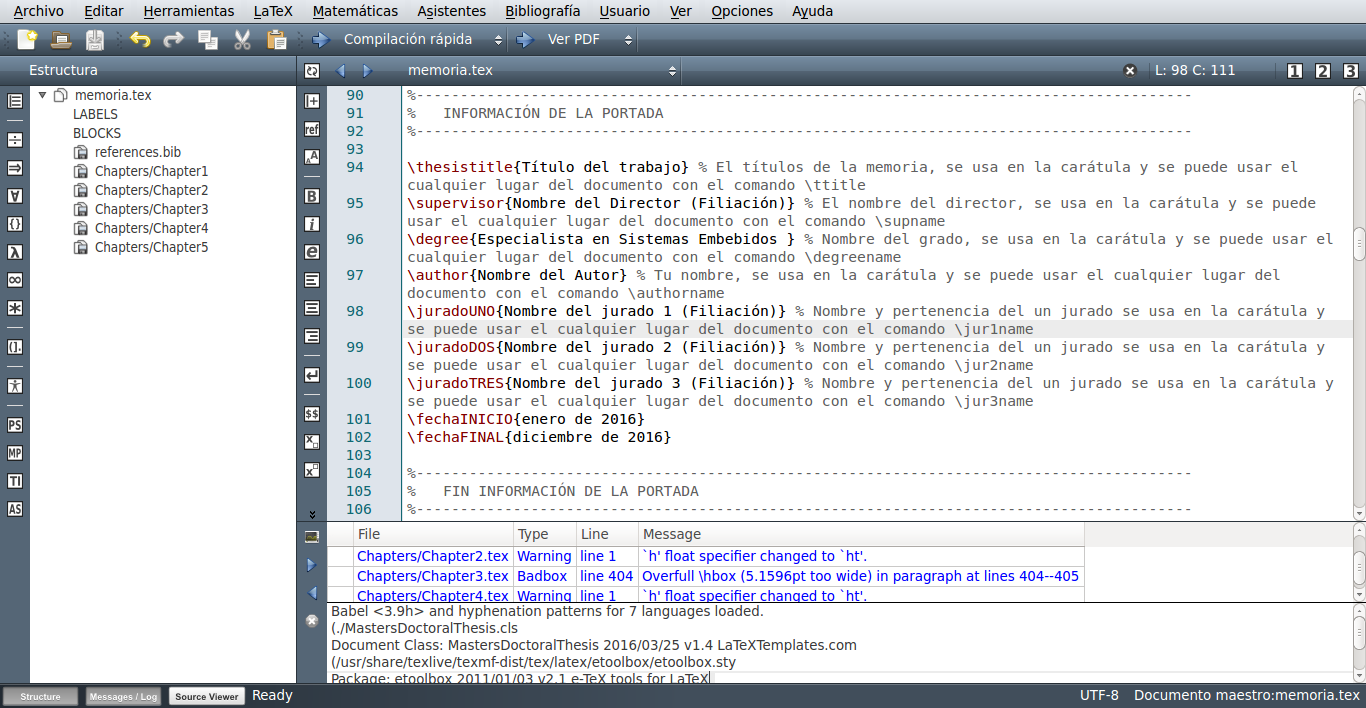
\includegraphics[width=.5\textwidth]{./Figures/texmaker.png}
	\caption{Entorno de trabajo de texMaker.}
	\label{fig:texmaker}
\end{figure}

\vspace{1cm}

Notar que existe una vista llamada Estructura a la izquierda de la interfaz que nos permite abrir desde dentro del programa los archivos individuales de los capítulos.  A la derecha se encuentra una vista con el archivo propiamente dicho para su edición. Hacia la parte inferior se encuentra una vista del log con información de los resultados de la compilación.  En esta última vista pueden aparecen advertencias o \textit{warning}, que normalmente pueden ser ignorados, y los errores que se indican en color rojo y deben resolverse para que se genere el PDF de salida.

Recordar que el archivo que se debe compilar con PDFLaTeX es \file{memoria.tex}, si se tratara de compilar alguno de los capítulos saldría un error.  Para salvar la molestia de tener que cambiar de archivo para compilar cada vez que se realice una modificación en un capítulo, se puede definir el archivo \file{memoria.tex} como ``documento maestro'' yendo al menú opciones -> ``definir documento actual como documento maestro'', lo que permite compilar con PDFLaTeX memoria.tex directamente desde cualquier archivo que se esté modificando . Se muestra esta opción en la figura \ref{fig:docMaestro}.

\begin{figure}[h]
	\centering
	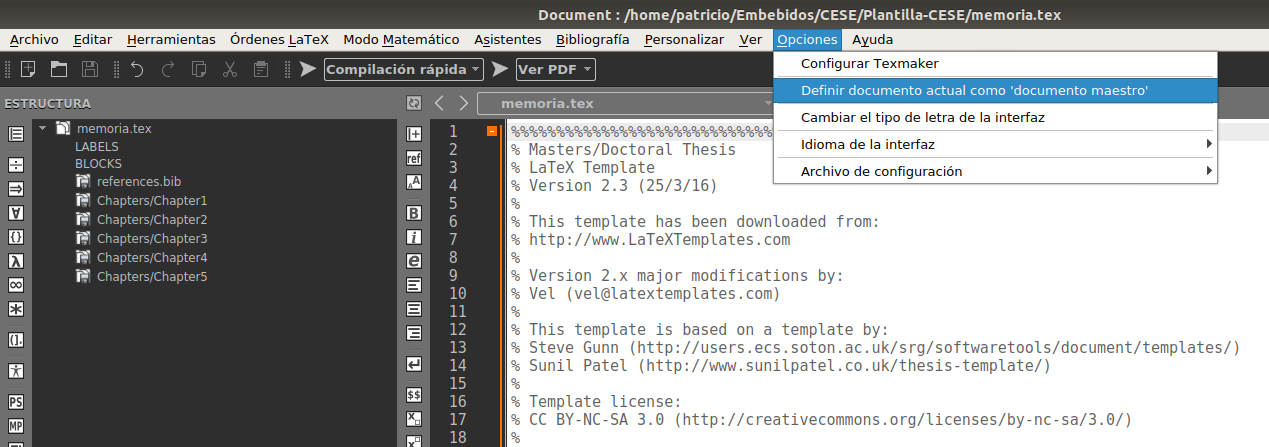
\includegraphics[width=\textwidth]{./Figures/docMaestro.png}
	\caption{Definir memoria.tex como documento maestro.}
	\label{fig:docMaestro}
\end{figure}

En el menú herramientas se encuentran las opciones de compilación.  Para producir un archivo PDF a partir de un archivo .tex se debe ejecutar PDFLaTeX (el shortcut es F6). Para incorporar nueva bibliografía se debe utilizar la opción BibTeX del mismo menú herramientas (el shortcut es F11).

Notar que para actualizar las tablas de contenidos se debe ejecutar PDFLaTeX dos veces.  Esto se debe a que es necesario actualizar algunos archivos auxiliares antes de obtener el resultado final.  En forma similar, para actualizar las referencias bibliográficas se debe ejecutar primero PDFLaTeX, después BibTeX y finalmente PDFLaTeX dos veces por idénticos motivos.

\section{Personalizando la plantilla, el archivo \file{memoria.tex}}
\label{sec:FillingFile}

Para personalizar la plantilla se debe incorporar la información propia en los distintos archivos \file{.tex}. 

Primero abrir \file{memoria.tex} con TexMaker (o el editor de su preferencia). Se debe ubicar dentro del archivo el bloque de código titulado \emph{INFORMACIÓN DE LA PORTADA} donde se deben incorporar los primeros datos personales con los que se construirá automáticamente la portada.


%----------------------------------------------------------------------------------------

\section{El código del archivo \file{memoria.tex} explicado}

El archivo \file{memoria.tex} contiene la estructura del documento y es el archivo de mayor jerarquía de la memoria.  Podría ser equiparable a la función \emph{main()} de un programa en C, o mejor dicho al archivo fuente .c donde se encuentra definida la función main().

La estructura básica de cualquier documento de \LaTeX{} comienza con la definición de clase del documento, es seguida por un preámbulo donde se pueden agregar funcionalidades con el uso de \texttt{paquetes} (equiparables a bibliotecas de C), y finalmente, termina con el cuerpo del documento, donde irá el contenido de la memoria.

\lstset{%
  basicstyle=\small\ttfamily,
  language=[LaTeX]{TeX}
}

\begin{lstlisting}
\documentclass{article}  <- Definicion de clase
\usepackage{listings}	 <- Preambulo

\begin{document}	 <- Comienzo del contenido propio 
	Hello world!
\end{document}
\end{lstlisting}


El archivo \file{memoria.tex} se encuentra densamente comentado para explicar qué páginas, secciones y elementos de formato está creando el código \LaTeX{} en cada línea. El código está dividido en bloques con nombres en mayúsculas para que resulte evidente qué es lo que hace esa porción de código en particular. Inicialmente puede parecer que hay mucho código \LaTeX{}, pero es principalmente código para dar formato a la memoria por lo que no requiere intervención del usuario de la plantilla.  Sí se deben personalizar con su información los bloques indicados como:

\begin{itemize}
	\item Informacion de la memoria
	\item Resumen
	\item Agradecimientos
	\item Dedicatoria
\end{itemize}

El índice de contenidos, las listas de figura de tablas se generan en forma automática y no requieren intervención ni edición manual por parte del usuario de la plantilla. 

En la parte final del documento se encuentran los capítulos y los apéndices.  Por defecto se incluyen los 5 capítulos propuestos que se encuentran en la carpeta /Chapters. Cada capítulo se debe escribir en un archivo .tex separado y se debe poner en la carpeta \emph{Chapters} con el nombre \file{Chapter1}, \file{Chapter2}, etc\ldots El código para incluir capítulos desde archivos externos se muestra a continuación.

\begin{verbatim}
	% Chapter 1

\chapter{Introducción general} % Main chapter title

\label{Chapter1} % For referencing the chapter elsewhere, use \ref{Chapter1} 
\label{IntroGeneral}

Todos los capítulos deben comenzar con un breve párrafo introductorio que indique cuál es el contenido que se encontrará al leerlo.  La redacción sobre el contenido de la memoria debe hacerse en presente y todo lo referido al proyecto en pasado, siempre de modo impersonal.

%----------------------------------------------------------------------------------------

% Define some commands to keep the formatting separated from the content 
\newcommand{\keyword}[1]{\textbf{#1}}
\newcommand{\tabhead}[1]{\textbf{#1}}
\newcommand{\code}[1]{\texttt{#1}}
\newcommand{\file}[1]{\texttt{\bfseries#1}}
\newcommand{\option}[1]{\texttt{\itshape#1}}
\newcommand{\grados}{$^{\circ}$}

%----------------------------------------------------------------------------------------

%\section{Introducción}

%----------------------------------------------------------------------------------------
\section{Aprendiendo \LaTeX{}}

\LaTeX{} no es \textsc{WYSIWYG} (What You See is What You Get), a diferencia de los procesadores de texto como Microsoft Word o Pages de Apple o incluso LibreOffice en el mundo open-source. En lugar de ello, un documento escrito para \LaTeX{} es en realidad un archivo de texto simple o llano que \emph{no contiene formato} . Nosotros le decimos a \LaTeX{} cómo deseamos que se aplique el formato en el documento final escribiendo comandos simples entre el texto, por ejemplo, si quiero usar texto en itálicas para dar énfasis, escribo \verb|\it{texto}| y pongo el texto que quiero en itálicas entre medio de las llaves. Esto significa que \LaTeX{} es un lenguaje del tipo \enquote{mark-up}, muy parecido a HTML.

\subsection{Una introducción (no tan corta) a \LaTeX{}}

Si sos nuevo en \LaTeX{}, hay un muy buen libro electrónico - disponible gratuitamente en Internet como un archivo PDF - llamado, \enquote{A (not so short) Introduction to \LaTeX{}}. El título del libro es generalmente acortado a simplemente \emph{lshort}. Puede descargar la versión más reciente en inglés (ya que se actualiza de vez en cuando) desde aquí:
\url{http://www.ctan.org/tex-archive/info/lshort/english/lshort.pdf}

Se puede encontrar la versión en español en la lista en esta página: \url{http://www.ctan.org/tex-archive/info/lshort/}

\subsubsection{Una subsubsección}

Acá tiene un ejemplo de una ``subsubsección'' que es el cuarto nivel de ordenamiento del texto, después de capítulo, sección y subsección.  Como se puede ver, las subsubsecciones no van numeradas en el cuerpo del documento ni en el índice.  El formato está definido por la plantilla y no debe ser modificado.

\subsection{Guía matemática rápida para \LaTeX{}}

Si estás escribiendo un documento con mucho contenido matemático, entonces es posible que desees leer el documento de la AMS (American Mathematical Society) llamado, \enquote{A Short Math Guide for \LaTeX{}}. Se puede encontrar en línea en el siguiente link: \url{http://www.ams.org/tex/amslatex.html} en la sección \enquote{Additional Documentation} hacia la parte inferior de la página.


%----------------------------------------------------------------------------------------

\section{Utilizando esta plantilla}

Si estás familiarizado con \LaTeX{}, entonces podés explorar la estructura de directorios de esta plantilla y proceder a personalizarla agregando tu información en el bloque \emph{INFORMACIÓN DE LA PORTADA} en el archivo \file{memoria.tex}.  

Se puede continuar luego modificando el resto de los archivos siguiendo los lineamientos que se describen en la sección \ref{sec:FillingFile} en la página \pageref{sec:FillingFile}.

Debés asegurarte de leer el capítulo \ref{Chapter2} acerca de las convenciones utilizadas para las Memoria de los Trabajos Finales de la \degreename.

Si sos nuevo en \LaTeX{}, se recomienda que continúes leyendo el documento ya que contiene información básica para aprovechar el potencial de esta herramienta.


%----------------------------------------------------------------------------------------

\section{Qué incluye esta plantilla}

\subsection{Carpetas}

Esta plantilla se distribuye como una único archivo .zip que se puede descomprimir en varios archivos y carpetas. Asimismo, se puede consultar el repositorio git para obtener la última versión de los archivos, \url{https://github.com/patriciobos/Plantilla-CESE.git}. Los nombres de las carpetas son, o pretender ser, auto-explicativos.

\keyword{Appendices} -- Esta es la carpeta donde se deben poner los apéndices. Cada apéndice debe ir en su propio archivo \file{.tex}. Se incluye un ejemplo y una plantilla en la carpeta.

\keyword{Chapters} -- Esta es la carpeta donde se deben poner los capítulos de la memoria. Cada capítulo debe ir un su propio archivo \file{.tex} por separado.  Se ofrece por defecto, la siguiente estructura de capítulos y se recomienda su utilización dentro de lo posible:

\begin{itemize}
\item Capítulo 1: Introducción general	
\item Capítulo 2: Introducción específica
\item Capítulo 3: Diseño e implementación
\item Capítulo 4: Ensayos y resultados
\item Capítulo 5: Conclusiones

\end{itemize}

Esta estructura de capítulos es la que se recomienda para las memorias de la especialización.

\keyword{Figures} -- Esta carpeta contiene todas las figuras de la memoria.  Estas son las versiones finales de las imágenes que van a ser incluidas en la memoria.  Pueden ser imágenes en formato \textit{raster}\footnote{\url{https://en.wikipedia.org/wiki/Raster_graphics}} como \file{.png}, \file{.jpg} o en formato vectoriales\footnote{\url{https://en.wikipedia.org/wiki/Vector_graphics}} como \file{.pdf}, \file{.ps}.  Se debe notar que utilizar imágenes vectoriales disminuye notablemente el peso del documento final y acelera el tiempo de compilación por lo que es recomendable su utilización siempre que sea posible.

\subsection{Archivos}

También están incluidos varios archivos, la mayoría de ellos son de texto plano y se puede ver su contenido en un editor de texto. Después de la compilación inicial, se verá que más archivos auxiliares son creados por \ LaTeX{} o BibTeX, pero son de uso interno y no es necesario hacer nada en particular con ellos.  Toda la información necesaria para compilar el documento se encuentra en los archivos \file{.tex}, \file{.bib}, \file{.cls} y en las imágenes de la carpeta Figures.

\keyword{referencias.bib} - este es un archivo importante que contiene toda la información de referencias bibliográficas que se utilizarán para las citas en la memoria en conjunto con BibTeX. Usted puede escribir las entradas bibliográficas en forma manual, aunque existen también programas de gestión de referencias que facilitan la creación y gestión de las referencias y permiten exportarlas en formato BibTeX.  También hay disponibles sitios web como \url{books.google.com} que permiten obtener toda la información necesaria para una cita en formato BibTeX. Ver sección \ref{sec:biblio}

\keyword{MastersDoctoralThesis.cls} -- este es un archivo importante. Es el archivos con la clase que le informa a \LaTeX{} cómo debe dar formato a la memoria. El usuario de la plantilla no debería necesitar modificar nada de este archivo.

\keyword{memoria.pdf} -- esta es su memoria con una tipografía bellamente compuesta (en formato de archivo PDF) creado por \LaTeX{}. Se distribuye con la plantilla y después de compilar por primera vez sin hacer ningún cambio se debería obtener una versión idéntica a este documento.

\keyword{memoria.tex} -- este es un archivo importante. Este es el archivo que tiene que compilar \LaTeX{} para producir la memoria como un archivo PDF. Contiene un marco de trabajo y estructuras que le indican a \LaTeX{} cómo diagramar la memoria.  Está altamente comentado para que se pueda entender qué es lo que realiza cada línea de código y por qué está incluida en ese lugar.  En este archivo se debe completar la información personalizada de las primeras sección según se indica en la sección \ref{sec:FillingFile}.

Archivos que \emph{no} forman parte de la distribución de la plantilla pero que son generados por \LaTeX{} como archivos auxiliares necesarios para la producción de la memoria.pdf son:

\keyword{memoria.aux} -- este es un archivo auxiliar generado por \LaTeX{}, si se borra \LaTeX{} simplemente lo regenera cuando se compila el archivo principal \file{memoria.tex}.

\keyword{memoria.bbl} -- este es un archivo auxiliar generado por BibTeX, si se borra BibTeX simplemente lo regenera cuando se compila el archivo principal \file{memoria.tex}. Mientras que el archivo \file{.bib} contiene todas las referencias que hay, este archivo \file{.bbl} contine sólo las referencias que han sido citadas y se utiliza para la construcción de la bibiografía.

\keyword{memoria.blg} -- este es un archivo auxiliar generado por BibTeX, si se borra BibTeX simplemente lo regenera cuando se compila el archivo principal \file{memoria.tex}.

\keyword{memoria.lof} -- este es un archivo auxiliar generado por \LaTeX{}, si se borra \LaTeX{} simplemente lo regenera cuando se compila el archivo principal \file{memoria.tex}.  Le indica a \LaTeX{} cómo construir la sección \emph{Lista de Figuras}.
 
\keyword{memoria.log} --  este es un archivo auxiliar generado por \LaTeX{}, si se borra \LaTeX{} simplemente lo regenera cuando se compila el archivo principal \file{memoria.tex}. Contiene mensajes de \LaTeX{}. Si se reciben errores o advertencias durante la compilación, se guardan en este archivo \file{.log}.

\keyword{memoria.lot} -- este es un archivo auxiliar generado por \LaTeX{}, si se borra \LaTeX{} simplemente lo regenera cuando se compila el archivo principal \file{memoria.tex}.  Le indica a \LaTeX{} cómo construir la sección \emph{Lista de Tablas}.

\keyword{memoria.out} -- este es un archivo auxiliar generado por \LaTeX{}, si se borra \LaTeX{} simplemente lo regenera cuando se compila el archivo principal \file{memoria.tex}.

De esta larga lista de archivos, sólo aquellos con la extensión \file{.bib}, \file{.cls} y \file{.tex} son importantes.  Los otros archivos auxiliares pueden ser ignorados o borrados ya que \LaTeX{} y BibTeX los regenerarán durante la compilación.

%----------------------------------------------------------------------------------------

\section{Entorno de trabajo}

Ante de comenzar a editar la plantilla debemos tener un editor \LaTeX{} instalado en nuestra computadora.  En forma análoga a lo que sucede en lenguaje C, que se puede crear y editar código con casi cualquier editor, existen ciertos entornos de trabajo que nos pueden simplificar mucho la tarea.  En este sentido, se recomienda, sobre todo para los principiantes en \LaTeX{} la utilización de TexMaker, un programa gratuito y multi-plantaforma que está disponible tanto para windows como para sistemas GNU/linux.

La versión más reciente de TexMaker es la 4.5 y se puede descargar del siguiente link: \url{http://www.xm1math.net/texmaker/download.html}. Se puede consultar el manual de usuario en el siguiente link: \url{http://www.xm1math.net/texmaker/doc.html}.
 

\subsection{Paquetes adicionales}

Si bien durante el proceso de instalación de TexMaker, o cualquier otro editor que se haya elegido, se instalarán en el sistema los paquetes básicos necesarios para trabajar con \LaTeX{}, la plantilla de los trabajos de Especialización y Maestría requieren de paquete adicionales.

Se indican a continuación los comandos que se deben introducir en la consola de Ubuntu (ctrl + alt + t) para instalarlos:

\begin{lstlisting}[language=bash]
  $ sudo apt install texlive-lang-spanish texlive-science 
  $ sudo apt install texlive-bibtex-extra biber
  $ sudo apt install texlive texlive-fonts-recommended
  $ sudo apt install texlive-latex-extra
\end{lstlisting}


\subsection{Configurando TexMaker}
\label{subsec:configurando}



Una vez instalado el programa y los paquetes adicionales se debe abrir el archivo memoria.tex con el editor para ver una pantalla similar a la que se puede apreciar en la figura \ref{fig:texmaker}. 
Una vez instalado el programa y los paquetes adicionales se debe abrir el archivo memoria.tex con el editor para ver una pantalla similar a la que se puede apreciar en la figura \ref{fig:texmaker}. 
Una vez instalado el programa y los paquetes adicionales se debe abrir el archivo memoria.tex con el editor para ver una pantalla similar a la que se puede apreciar en la figura \ref{fig:texmaker}. 
Una vez instalado el programa y los paquetes adicionales se debe abrir el archivo memoria.tex con el editor para ver una pantalla similar a la que se puede apreciar en la figura \ref{fig:texmaker}. 

\vspace{1cm}

\begin{figure}[htbp]
	\centering
	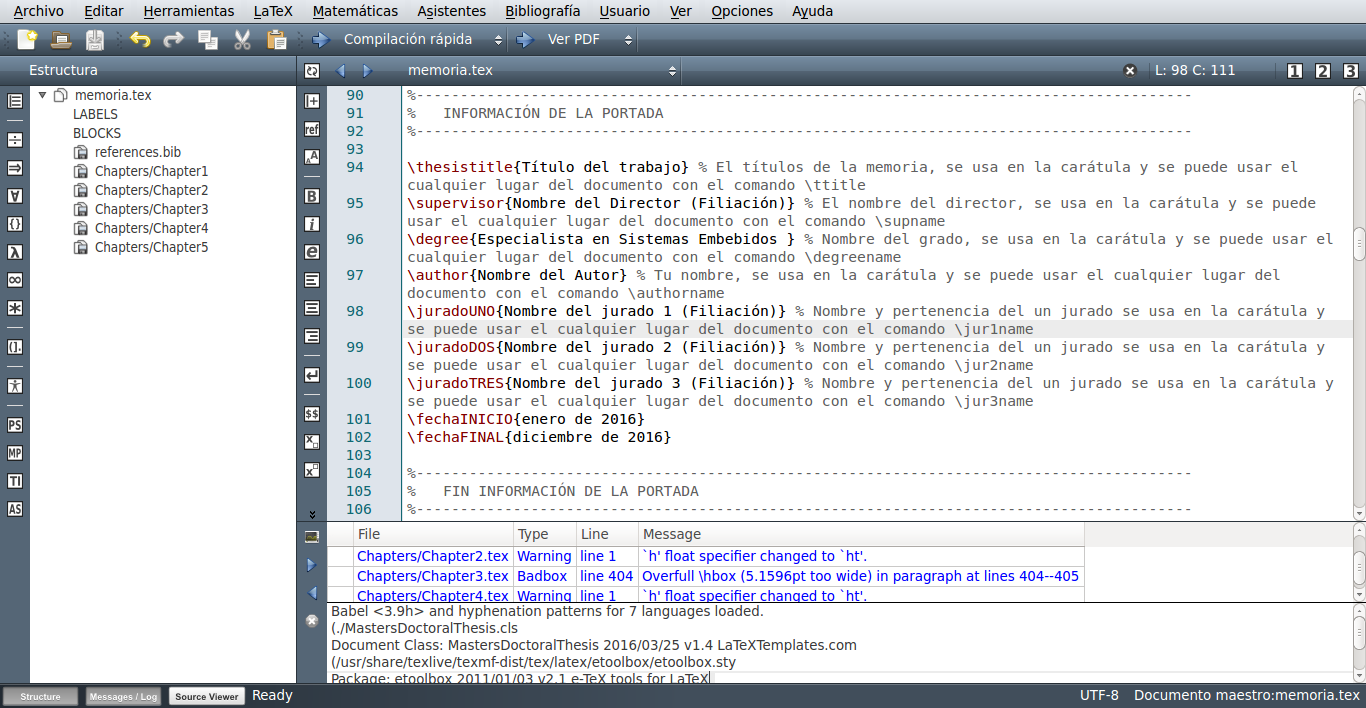
\includegraphics[width=.5\textwidth]{./Figures/texmaker.png}
	\caption{Entorno de trabajo de texMaker.}
	\label{fig:texmaker}
\end{figure}

\vspace{1cm}

Notar que existe una vista llamada Estructura a la izquierda de la interfaz que nos permite abrir desde dentro del programa los archivos individuales de los capítulos.  A la derecha se encuentra una vista con el archivo propiamente dicho para su edición. Hacia la parte inferior se encuentra una vista del log con información de los resultados de la compilación.  En esta última vista pueden aparecen advertencias o \textit{warning}, que normalmente pueden ser ignorados, y los errores que se indican en color rojo y deben resolverse para que se genere el PDF de salida.

Recordar que el archivo que se debe compilar con PDFLaTeX es \file{memoria.tex}, si se tratara de compilar alguno de los capítulos saldría un error.  Para salvar la molestia de tener que cambiar de archivo para compilar cada vez que se realice una modificación en un capítulo, se puede definir el archivo \file{memoria.tex} como ``documento maestro'' yendo al menú opciones -> ``definir documento actual como documento maestro'', lo que permite compilar con PDFLaTeX memoria.tex directamente desde cualquier archivo que se esté modificando . Se muestra esta opción en la figura \ref{fig:docMaestro}.

\begin{figure}[h]
	\centering
	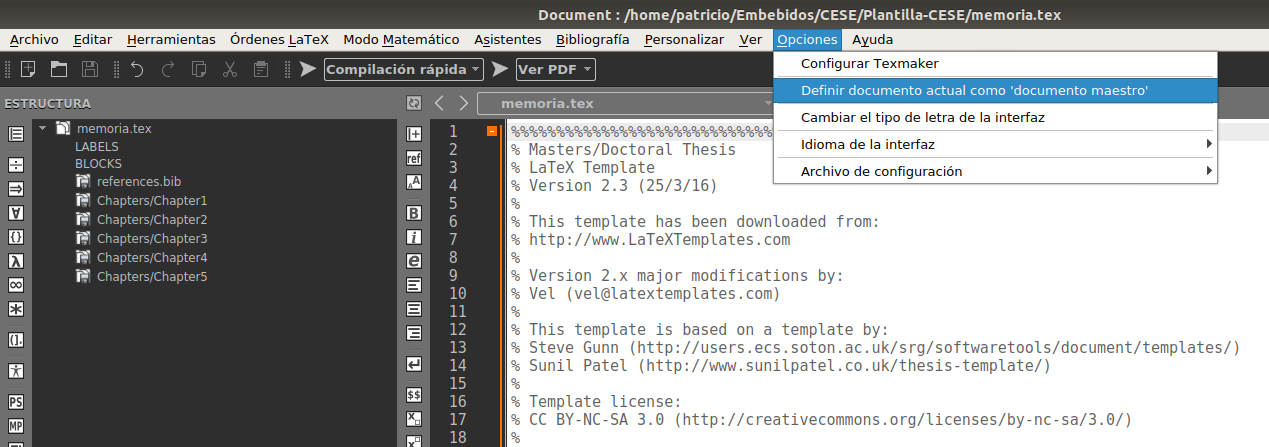
\includegraphics[width=\textwidth]{./Figures/docMaestro.png}
	\caption{Definir memoria.tex como documento maestro.}
	\label{fig:docMaestro}
\end{figure}

En el menú herramientas se encuentran las opciones de compilación.  Para producir un archivo PDF a partir de un archivo .tex se debe ejecutar PDFLaTeX (el shortcut es F6). Para incorporar nueva bibliografía se debe utilizar la opción BibTeX del mismo menú herramientas (el shortcut es F11).

Notar que para actualizar las tablas de contenidos se debe ejecutar PDFLaTeX dos veces.  Esto se debe a que es necesario actualizar algunos archivos auxiliares antes de obtener el resultado final.  En forma similar, para actualizar las referencias bibliográficas se debe ejecutar primero PDFLaTeX, después BibTeX y finalmente PDFLaTeX dos veces por idénticos motivos.

\section{Personalizando la plantilla, el archivo \file{memoria.tex}}
\label{sec:FillingFile}

Para personalizar la plantilla se debe incorporar la información propia en los distintos archivos \file{.tex}. 

Primero abrir \file{memoria.tex} con TexMaker (o el editor de su preferencia). Se debe ubicar dentro del archivo el bloque de código titulado \emph{INFORMACIÓN DE LA PORTADA} donde se deben incorporar los primeros datos personales con los que se construirá automáticamente la portada.


%----------------------------------------------------------------------------------------

\section{El código del archivo \file{memoria.tex} explicado}

El archivo \file{memoria.tex} contiene la estructura del documento y es el archivo de mayor jerarquía de la memoria.  Podría ser equiparable a la función \emph{main()} de un programa en C, o mejor dicho al archivo fuente .c donde se encuentra definida la función main().

La estructura básica de cualquier documento de \LaTeX{} comienza con la definición de clase del documento, es seguida por un preámbulo donde se pueden agregar funcionalidades con el uso de \texttt{paquetes} (equiparables a bibliotecas de C), y finalmente, termina con el cuerpo del documento, donde irá el contenido de la memoria.

\lstset{%
  basicstyle=\small\ttfamily,
  language=[LaTeX]{TeX}
}

\begin{lstlisting}
\documentclass{article}  <- Definicion de clase
\usepackage{listings}	 <- Preambulo

\begin{document}	 <- Comienzo del contenido propio 
	Hello world!
\end{document}
\end{lstlisting}


El archivo \file{memoria.tex} se encuentra densamente comentado para explicar qué páginas, secciones y elementos de formato está creando el código \LaTeX{} en cada línea. El código está dividido en bloques con nombres en mayúsculas para que resulte evidente qué es lo que hace esa porción de código en particular. Inicialmente puede parecer que hay mucho código \LaTeX{}, pero es principalmente código para dar formato a la memoria por lo que no requiere intervención del usuario de la plantilla.  Sí se deben personalizar con su información los bloques indicados como:

\begin{itemize}
	\item Informacion de la memoria
	\item Resumen
	\item Agradecimientos
	\item Dedicatoria
\end{itemize}

El índice de contenidos, las listas de figura de tablas se generan en forma automática y no requieren intervención ni edición manual por parte del usuario de la plantilla. 

En la parte final del documento se encuentran los capítulos y los apéndices.  Por defecto se incluyen los 5 capítulos propuestos que se encuentran en la carpeta /Chapters. Cada capítulo se debe escribir en un archivo .tex separado y se debe poner en la carpeta \emph{Chapters} con el nombre \file{Chapter1}, \file{Chapter2}, etc\ldots El código para incluir capítulos desde archivos externos se muestra a continuación.

\begin{verbatim}
	% Chapter 1

\chapter{Introducción general} % Main chapter title

\label{Chapter1} % For referencing the chapter elsewhere, use \ref{Chapter1} 
\label{IntroGeneral}

Todos los capítulos deben comenzar con un breve párrafo introductorio que indique cuál es el contenido que se encontrará al leerlo.  La redacción sobre el contenido de la memoria debe hacerse en presente y todo lo referido al proyecto en pasado, siempre de modo impersonal.

%----------------------------------------------------------------------------------------

% Define some commands to keep the formatting separated from the content 
\newcommand{\keyword}[1]{\textbf{#1}}
\newcommand{\tabhead}[1]{\textbf{#1}}
\newcommand{\code}[1]{\texttt{#1}}
\newcommand{\file}[1]{\texttt{\bfseries#1}}
\newcommand{\option}[1]{\texttt{\itshape#1}}
\newcommand{\grados}{$^{\circ}$}

%----------------------------------------------------------------------------------------

%\section{Introducción}

%----------------------------------------------------------------------------------------
\section{Aprendiendo \LaTeX{}}

\LaTeX{} no es \textsc{WYSIWYG} (What You See is What You Get), a diferencia de los procesadores de texto como Microsoft Word o Pages de Apple o incluso LibreOffice en el mundo open-source. En lugar de ello, un documento escrito para \LaTeX{} es en realidad un archivo de texto simple o llano que \emph{no contiene formato} . Nosotros le decimos a \LaTeX{} cómo deseamos que se aplique el formato en el documento final escribiendo comandos simples entre el texto, por ejemplo, si quiero usar texto en itálicas para dar énfasis, escribo \verb|\it{texto}| y pongo el texto que quiero en itálicas entre medio de las llaves. Esto significa que \LaTeX{} es un lenguaje del tipo \enquote{mark-up}, muy parecido a HTML.

\subsection{Una introducción (no tan corta) a \LaTeX{}}

Si sos nuevo en \LaTeX{}, hay un muy buen libro electrónico - disponible gratuitamente en Internet como un archivo PDF - llamado, \enquote{A (not so short) Introduction to \LaTeX{}}. El título del libro es generalmente acortado a simplemente \emph{lshort}. Puede descargar la versión más reciente en inglés (ya que se actualiza de vez en cuando) desde aquí:
\url{http://www.ctan.org/tex-archive/info/lshort/english/lshort.pdf}

Se puede encontrar la versión en español en la lista en esta página: \url{http://www.ctan.org/tex-archive/info/lshort/}

\subsubsection{Una subsubsección}

Acá tiene un ejemplo de una ``subsubsección'' que es el cuarto nivel de ordenamiento del texto, después de capítulo, sección y subsección.  Como se puede ver, las subsubsecciones no van numeradas en el cuerpo del documento ni en el índice.  El formato está definido por la plantilla y no debe ser modificado.

\subsection{Guía matemática rápida para \LaTeX{}}

Si estás escribiendo un documento con mucho contenido matemático, entonces es posible que desees leer el documento de la AMS (American Mathematical Society) llamado, \enquote{A Short Math Guide for \LaTeX{}}. Se puede encontrar en línea en el siguiente link: \url{http://www.ams.org/tex/amslatex.html} en la sección \enquote{Additional Documentation} hacia la parte inferior de la página.


%----------------------------------------------------------------------------------------

\section{Utilizando esta plantilla}

Si estás familiarizado con \LaTeX{}, entonces podés explorar la estructura de directorios de esta plantilla y proceder a personalizarla agregando tu información en el bloque \emph{INFORMACIÓN DE LA PORTADA} en el archivo \file{memoria.tex}.  

Se puede continuar luego modificando el resto de los archivos siguiendo los lineamientos que se describen en la sección \ref{sec:FillingFile} en la página \pageref{sec:FillingFile}.

Debés asegurarte de leer el capítulo \ref{Chapter2} acerca de las convenciones utilizadas para las Memoria de los Trabajos Finales de la \degreename.

Si sos nuevo en \LaTeX{}, se recomienda que continúes leyendo el documento ya que contiene información básica para aprovechar el potencial de esta herramienta.


%----------------------------------------------------------------------------------------

\section{Qué incluye esta plantilla}

\subsection{Carpetas}

Esta plantilla se distribuye como una único archivo .zip que se puede descomprimir en varios archivos y carpetas. Asimismo, se puede consultar el repositorio git para obtener la última versión de los archivos, \url{https://github.com/patriciobos/Plantilla-CESE.git}. Los nombres de las carpetas son, o pretender ser, auto-explicativos.

\keyword{Appendices} -- Esta es la carpeta donde se deben poner los apéndices. Cada apéndice debe ir en su propio archivo \file{.tex}. Se incluye un ejemplo y una plantilla en la carpeta.

\keyword{Chapters} -- Esta es la carpeta donde se deben poner los capítulos de la memoria. Cada capítulo debe ir un su propio archivo \file{.tex} por separado.  Se ofrece por defecto, la siguiente estructura de capítulos y se recomienda su utilización dentro de lo posible:

\begin{itemize}
\item Capítulo 1: Introducción general	
\item Capítulo 2: Introducción específica
\item Capítulo 3: Diseño e implementación
\item Capítulo 4: Ensayos y resultados
\item Capítulo 5: Conclusiones

\end{itemize}

Esta estructura de capítulos es la que se recomienda para las memorias de la especialización.

\keyword{Figures} -- Esta carpeta contiene todas las figuras de la memoria.  Estas son las versiones finales de las imágenes que van a ser incluidas en la memoria.  Pueden ser imágenes en formato \textit{raster}\footnote{\url{https://en.wikipedia.org/wiki/Raster_graphics}} como \file{.png}, \file{.jpg} o en formato vectoriales\footnote{\url{https://en.wikipedia.org/wiki/Vector_graphics}} como \file{.pdf}, \file{.ps}.  Se debe notar que utilizar imágenes vectoriales disminuye notablemente el peso del documento final y acelera el tiempo de compilación por lo que es recomendable su utilización siempre que sea posible.

\subsection{Archivos}

También están incluidos varios archivos, la mayoría de ellos son de texto plano y se puede ver su contenido en un editor de texto. Después de la compilación inicial, se verá que más archivos auxiliares son creados por \ LaTeX{} o BibTeX, pero son de uso interno y no es necesario hacer nada en particular con ellos.  Toda la información necesaria para compilar el documento se encuentra en los archivos \file{.tex}, \file{.bib}, \file{.cls} y en las imágenes de la carpeta Figures.

\keyword{referencias.bib} - este es un archivo importante que contiene toda la información de referencias bibliográficas que se utilizarán para las citas en la memoria en conjunto con BibTeX. Usted puede escribir las entradas bibliográficas en forma manual, aunque existen también programas de gestión de referencias que facilitan la creación y gestión de las referencias y permiten exportarlas en formato BibTeX.  También hay disponibles sitios web como \url{books.google.com} que permiten obtener toda la información necesaria para una cita en formato BibTeX. Ver sección \ref{sec:biblio}

\keyword{MastersDoctoralThesis.cls} -- este es un archivo importante. Es el archivos con la clase que le informa a \LaTeX{} cómo debe dar formato a la memoria. El usuario de la plantilla no debería necesitar modificar nada de este archivo.

\keyword{memoria.pdf} -- esta es su memoria con una tipografía bellamente compuesta (en formato de archivo PDF) creado por \LaTeX{}. Se distribuye con la plantilla y después de compilar por primera vez sin hacer ningún cambio se debería obtener una versión idéntica a este documento.

\keyword{memoria.tex} -- este es un archivo importante. Este es el archivo que tiene que compilar \LaTeX{} para producir la memoria como un archivo PDF. Contiene un marco de trabajo y estructuras que le indican a \LaTeX{} cómo diagramar la memoria.  Está altamente comentado para que se pueda entender qué es lo que realiza cada línea de código y por qué está incluida en ese lugar.  En este archivo se debe completar la información personalizada de las primeras sección según se indica en la sección \ref{sec:FillingFile}.

Archivos que \emph{no} forman parte de la distribución de la plantilla pero que son generados por \LaTeX{} como archivos auxiliares necesarios para la producción de la memoria.pdf son:

\keyword{memoria.aux} -- este es un archivo auxiliar generado por \LaTeX{}, si se borra \LaTeX{} simplemente lo regenera cuando se compila el archivo principal \file{memoria.tex}.

\keyword{memoria.bbl} -- este es un archivo auxiliar generado por BibTeX, si se borra BibTeX simplemente lo regenera cuando se compila el archivo principal \file{memoria.tex}. Mientras que el archivo \file{.bib} contiene todas las referencias que hay, este archivo \file{.bbl} contine sólo las referencias que han sido citadas y se utiliza para la construcción de la bibiografía.

\keyword{memoria.blg} -- este es un archivo auxiliar generado por BibTeX, si se borra BibTeX simplemente lo regenera cuando se compila el archivo principal \file{memoria.tex}.

\keyword{memoria.lof} -- este es un archivo auxiliar generado por \LaTeX{}, si se borra \LaTeX{} simplemente lo regenera cuando se compila el archivo principal \file{memoria.tex}.  Le indica a \LaTeX{} cómo construir la sección \emph{Lista de Figuras}.
 
\keyword{memoria.log} --  este es un archivo auxiliar generado por \LaTeX{}, si se borra \LaTeX{} simplemente lo regenera cuando se compila el archivo principal \file{memoria.tex}. Contiene mensajes de \LaTeX{}. Si se reciben errores o advertencias durante la compilación, se guardan en este archivo \file{.log}.

\keyword{memoria.lot} -- este es un archivo auxiliar generado por \LaTeX{}, si se borra \LaTeX{} simplemente lo regenera cuando se compila el archivo principal \file{memoria.tex}.  Le indica a \LaTeX{} cómo construir la sección \emph{Lista de Tablas}.

\keyword{memoria.out} -- este es un archivo auxiliar generado por \LaTeX{}, si se borra \LaTeX{} simplemente lo regenera cuando se compila el archivo principal \file{memoria.tex}.

De esta larga lista de archivos, sólo aquellos con la extensión \file{.bib}, \file{.cls} y \file{.tex} son importantes.  Los otros archivos auxiliares pueden ser ignorados o borrados ya que \LaTeX{} y BibTeX los regenerarán durante la compilación.

%----------------------------------------------------------------------------------------

\section{Entorno de trabajo}

Ante de comenzar a editar la plantilla debemos tener un editor \LaTeX{} instalado en nuestra computadora.  En forma análoga a lo que sucede en lenguaje C, que se puede crear y editar código con casi cualquier editor, existen ciertos entornos de trabajo que nos pueden simplificar mucho la tarea.  En este sentido, se recomienda, sobre todo para los principiantes en \LaTeX{} la utilización de TexMaker, un programa gratuito y multi-plantaforma que está disponible tanto para windows como para sistemas GNU/linux.

La versión más reciente de TexMaker es la 4.5 y se puede descargar del siguiente link: \url{http://www.xm1math.net/texmaker/download.html}. Se puede consultar el manual de usuario en el siguiente link: \url{http://www.xm1math.net/texmaker/doc.html}.
 

\subsection{Paquetes adicionales}

Si bien durante el proceso de instalación de TexMaker, o cualquier otro editor que se haya elegido, se instalarán en el sistema los paquetes básicos necesarios para trabajar con \LaTeX{}, la plantilla de los trabajos de Especialización y Maestría requieren de paquete adicionales.

Se indican a continuación los comandos que se deben introducir en la consola de Ubuntu (ctrl + alt + t) para instalarlos:

\begin{lstlisting}[language=bash]
  $ sudo apt install texlive-lang-spanish texlive-science 
  $ sudo apt install texlive-bibtex-extra biber
  $ sudo apt install texlive texlive-fonts-recommended
  $ sudo apt install texlive-latex-extra
\end{lstlisting}


\subsection{Configurando TexMaker}
\label{subsec:configurando}



Una vez instalado el programa y los paquetes adicionales se debe abrir el archivo memoria.tex con el editor para ver una pantalla similar a la que se puede apreciar en la figura \ref{fig:texmaker}. 
Una vez instalado el programa y los paquetes adicionales se debe abrir el archivo memoria.tex con el editor para ver una pantalla similar a la que se puede apreciar en la figura \ref{fig:texmaker}. 
Una vez instalado el programa y los paquetes adicionales se debe abrir el archivo memoria.tex con el editor para ver una pantalla similar a la que se puede apreciar en la figura \ref{fig:texmaker}. 
Una vez instalado el programa y los paquetes adicionales se debe abrir el archivo memoria.tex con el editor para ver una pantalla similar a la que se puede apreciar en la figura \ref{fig:texmaker}. 

\vspace{1cm}

\begin{figure}[htbp]
	\centering
	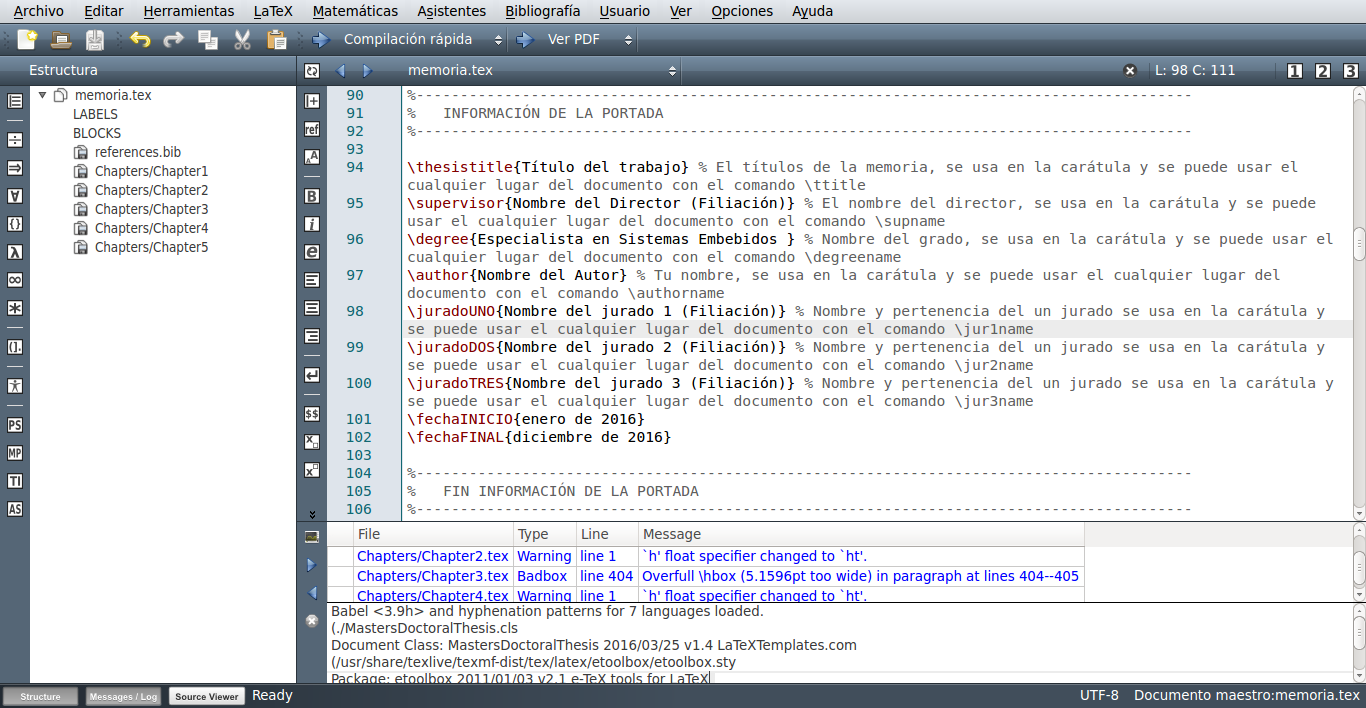
\includegraphics[width=.5\textwidth]{./Figures/texmaker.png}
	\caption{Entorno de trabajo de texMaker.}
	\label{fig:texmaker}
\end{figure}

\vspace{1cm}

Notar que existe una vista llamada Estructura a la izquierda de la interfaz que nos permite abrir desde dentro del programa los archivos individuales de los capítulos.  A la derecha se encuentra una vista con el archivo propiamente dicho para su edición. Hacia la parte inferior se encuentra una vista del log con información de los resultados de la compilación.  En esta última vista pueden aparecen advertencias o \textit{warning}, que normalmente pueden ser ignorados, y los errores que se indican en color rojo y deben resolverse para que se genere el PDF de salida.

Recordar que el archivo que se debe compilar con PDFLaTeX es \file{memoria.tex}, si se tratara de compilar alguno de los capítulos saldría un error.  Para salvar la molestia de tener que cambiar de archivo para compilar cada vez que se realice una modificación en un capítulo, se puede definir el archivo \file{memoria.tex} como ``documento maestro'' yendo al menú opciones -> ``definir documento actual como documento maestro'', lo que permite compilar con PDFLaTeX memoria.tex directamente desde cualquier archivo que se esté modificando . Se muestra esta opción en la figura \ref{fig:docMaestro}.

\begin{figure}[h]
	\centering
	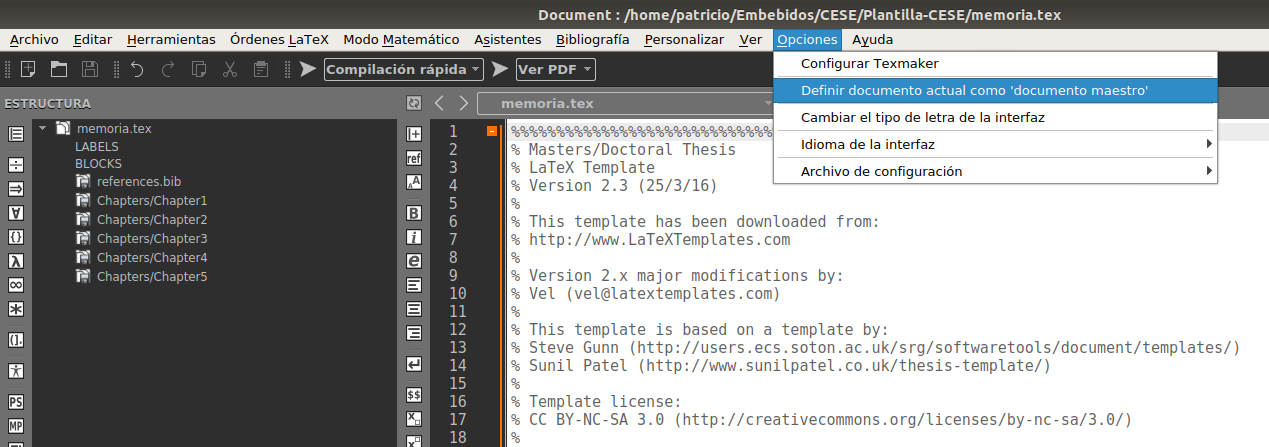
\includegraphics[width=\textwidth]{./Figures/docMaestro.png}
	\caption{Definir memoria.tex como documento maestro.}
	\label{fig:docMaestro}
\end{figure}

En el menú herramientas se encuentran las opciones de compilación.  Para producir un archivo PDF a partir de un archivo .tex se debe ejecutar PDFLaTeX (el shortcut es F6). Para incorporar nueva bibliografía se debe utilizar la opción BibTeX del mismo menú herramientas (el shortcut es F11).

Notar que para actualizar las tablas de contenidos se debe ejecutar PDFLaTeX dos veces.  Esto se debe a que es necesario actualizar algunos archivos auxiliares antes de obtener el resultado final.  En forma similar, para actualizar las referencias bibliográficas se debe ejecutar primero PDFLaTeX, después BibTeX y finalmente PDFLaTeX dos veces por idénticos motivos.

\section{Personalizando la plantilla, el archivo \file{memoria.tex}}
\label{sec:FillingFile}

Para personalizar la plantilla se debe incorporar la información propia en los distintos archivos \file{.tex}. 

Primero abrir \file{memoria.tex} con TexMaker (o el editor de su preferencia). Se debe ubicar dentro del archivo el bloque de código titulado \emph{INFORMACIÓN DE LA PORTADA} donde se deben incorporar los primeros datos personales con los que se construirá automáticamente la portada.


%----------------------------------------------------------------------------------------

\section{El código del archivo \file{memoria.tex} explicado}

El archivo \file{memoria.tex} contiene la estructura del documento y es el archivo de mayor jerarquía de la memoria.  Podría ser equiparable a la función \emph{main()} de un programa en C, o mejor dicho al archivo fuente .c donde se encuentra definida la función main().

La estructura básica de cualquier documento de \LaTeX{} comienza con la definición de clase del documento, es seguida por un preámbulo donde se pueden agregar funcionalidades con el uso de \texttt{paquetes} (equiparables a bibliotecas de C), y finalmente, termina con el cuerpo del documento, donde irá el contenido de la memoria.

\lstset{%
  basicstyle=\small\ttfamily,
  language=[LaTeX]{TeX}
}

\begin{lstlisting}
\documentclass{article}  <- Definicion de clase
\usepackage{listings}	 <- Preambulo

\begin{document}	 <- Comienzo del contenido propio 
	Hello world!
\end{document}
\end{lstlisting}


El archivo \file{memoria.tex} se encuentra densamente comentado para explicar qué páginas, secciones y elementos de formato está creando el código \LaTeX{} en cada línea. El código está dividido en bloques con nombres en mayúsculas para que resulte evidente qué es lo que hace esa porción de código en particular. Inicialmente puede parecer que hay mucho código \LaTeX{}, pero es principalmente código para dar formato a la memoria por lo que no requiere intervención del usuario de la plantilla.  Sí se deben personalizar con su información los bloques indicados como:

\begin{itemize}
	\item Informacion de la memoria
	\item Resumen
	\item Agradecimientos
	\item Dedicatoria
\end{itemize}

El índice de contenidos, las listas de figura de tablas se generan en forma automática y no requieren intervención ni edición manual por parte del usuario de la plantilla. 

En la parte final del documento se encuentran los capítulos y los apéndices.  Por defecto se incluyen los 5 capítulos propuestos que se encuentran en la carpeta /Chapters. Cada capítulo se debe escribir en un archivo .tex separado y se debe poner en la carpeta \emph{Chapters} con el nombre \file{Chapter1}, \file{Chapter2}, etc\ldots El código para incluir capítulos desde archivos externos se muestra a continuación.

\begin{verbatim}
	\include{Chapters/Chapter1}
	\include{Chapters/Chapter2} 
	\include{Chapters/Chapter3}
	\include{Chapters/Chapter4} 
	\include{Chapters/Chapter5} 
\end{verbatim}

Los apéndices también deben escribirse en archivos .tex separados, que se deben ubicar dentro de la carpeta \emph{Appendices}. Los apéndices vienen comentados por defecto con el caracter \code{\%} y para incluirlos simplemente se debe eliminar dicho caracter.

Finalmente, se encuentra el código para incluir la bibliografía en el documento final.  Este código tampoco debe modificarse. La metodología para trabajar las referencias bibliográficas se desarrolla en la sección \ref{sec:biblio}.
%----------------------------------------------------------------------------------------

\section{Bibliografía}
\label{sec:biblio}

Las opciones de formato de la bibliografía se controlan a través del paquete de latex \option{biblatex} que se incluye en la memoria en el archivo memoria.tex.  Estas opciones determinan cómo se generan las citas bibliográficas en el cuerpo del documento y cómo se genera la bibliografía al final de la memoria.

En el preámbulo se puede encontrar el código que incluye el paquete biblatex, que no requiere ninguna modificación del usuario de la plantilla, y que contiene las siguientes opciones:

\begin{lstlisting}
\usepackage[backend=bibtex,
	natbib=true, 
	style=numeric, 
	sorting=none]
{biblatex}
\end{lstlisting}

En el archivo \file{reference.bib} se encuentran las referencias bibliográficas que se pueden citar en el documento.  Para incorporar una nueva cita al documento lo primero es agregarla en este archivo con todos los campos necesario.  Todas las entradas bibliográficas comienzan con $@$ y una palabra que define el formato de la entrada.  Para cada formato existen campos obligatorios que deben completarse. No importa el orden en que las entradas estén definidas en el archivo .bib.  Tampoco es importante el orden en que estén definidos los campos de una entrada bibliográfica. A continuación se muestran algunos ejemplos:

\begin{lstlisting}
@ARTICLE{ARTICLE:1,
    AUTHOR="John Doe",
    TITLE="Title",
    JOURNAL="Journal",
    YEAR="2017",
}
\end{lstlisting}


\begin{lstlisting}
@BOOK{BOOK:1,
    AUTHOR="John Doe",
    TITLE="The Book without Title",
    PUBLISHER="Dummy Publisher",
    YEAR="2100",
}
\end{lstlisting}


\begin{lstlisting}
@INBOOK{BOOK:2,
    AUTHOR="John Doe",
    TITLE="The Book without Title",
    PUBLISHER="Dummy Publisher",
    YEAR="2100",
    PAGES="100-200",
}
\end{lstlisting}


\begin{lstlisting}
@MISC{WEBSITE:1,
    HOWPUBLISHED = "\url{http://example.com}",
    AUTHOR = "Intel",
    TITLE = "Example Website",
    MONTH = "12",
    YEAR = "1988",
    URLDATE = {2012-11-26}
}
\end{lstlisting}

Se debe notar que los nombres \emph{ARTICLE:1}, \emph{BOOK:1}, \emph{BOOK:2} y \emph{WEBSITE:1} son nombres de fantasía que le sirve al autor del documento para identificar la entrada. En este sentido, se podrían reemplazar por cualquier otro nombre.  Tampoco es necesario poner : seguido de un número, en los ejemplos sólo se incluye como un posible estilo para identificar las entradas.

La entradas se citan en el documento con el comando: 

\begin{verbatim}
\citep{nombre_de_la_entrada}
\end{verbatim}

Y cuando se usan, se muestran así: \citep{ARTICLE:1}, \citep{BOOK:1}, \citep{BOOK:2}, \citep{WEBSITE:1}.  Notar cómo se conforma la sección Bibliografía al final del documento.

Finalmente y como se mencionó en la subsección \ref{subsec:configurando}, para actualizar las referencias bibliográficas tanto en la sección bibliografía como las citas en el cuerpo del documento, se deben ejecutar las herramientas de compilación PDFLaTeX, BibTeX, PDFLaTeX, PDFLaTeX, en ese orden.  Este procedimiento debería resolver cualquier mensaje "Citation xxxxx on page x undefined".

	\chapter{Introducción específica} % Main chapter title

\label{Chapter2}

%----------------------------------------------------------------------------------------
%	SECTION 1
%----------------------------------------------------------------------------------------
En este capítulo se profundiza en aquellos aspectos clave para el desarrollo de este trabajo.
En primer lugar, se presentan los requerimientos de sistema y se amplía la información acerca de los modelos de 
inteligencia artificial que se han utilizado.
Finalmente, se expone el conjunto de técnicas y herramientas que se han aplicado a dichos modelos.

\section{Requerimientos del sistema}
Para llevar a cabo este trabajo
se identificaron una serie de requerimientos fundamentales.
A continuación se listan aquellos que están directamente relacionados con la implementación:

\begin{enumerate}
	\item Requerimientos del servidor:
	      \begin{enumerate}
		      \item El servidor debe alojar y administrar la información relativa al \textit{dataset} y la configuración del modelo LLM.
		      \item El servidor debe contar con los \textit{prompts} necesarios para especializar la respuesta de  la inteligencia artificial.
		      \item Al ser desplegado, el servidor deberá acceder al módulo LLM y utilizarlo en el procesamiento de peticiones entrantes.
		      \item El servidor debe dar acceso a clientes externos a través del protocolo API REST.
		      \item Los servicios REST deben aceptar entrada de texto en varios formatos: pdf, txt, docx o texto plano en el cuerpo de la petición.
		      \item Los servicios REST devolverán la respuesta en formato simple HTML para su cómoda visualización en un navegador.
		      \item El prototipo del servidor debe de tener una disponibilidad del 100\% durante la demostración.
	      \end{enumerate}
	\item Requerimientos del módulo LLM:
	      \begin{enumerate}
		      \item El módulo LLM debe aceptar entrada de texto y generar texto como salida.
		      \item En caso de que el texto de entrada sea legible, el módulo LLM debe aportar una respuesta con un detalle y profundidad razonables,
		            además de ser coherente con las instrucciones recibidas.
		      \item El módulo se ajustará a los \textit{prompts} recibidos para que, con el mismo contexto,
			  		devuelva información enfocada en un aspecto específico de la narrativa.
		      \item El tiempo de respuesta del módulo LLM debe estar en un rango de tiempo razonable para un servicio REST (no más de 5 minutos).
	      \end{enumerate}
\end{enumerate}

%----------------------------------------------------------------------------------------
%	SECTION 2
%----------------------------------------------------------------------------------------

\section{Modelos extensos de lenguaje}
Para abordar los requisitos de generación de texto resultó fundamental la utilización 
de modelos extensos de lenguaje, comúnmente denominados \textit{Large Language Models} (LLM).
Estos modelos son entrenados sobre enormes volúmenes de datos textuales para especializarlos
en predecir la secuencia de texto más probable dada una entrada previa.
Esta habilidad les permite generar texto de forma coherente con el contexto
al adaptarse al tono, estilo y contenido esperado.

Los LLM se basan en redes neuronales profundas que manejan miles de millones de parámetros
(lo que justifica su clasificación como modelos ``extensos'') para identificar patrones complejos del lenguaje natural \cite{att_is_all_you_need}. 
Estos modelos utilizan \textit{tokens} como unidad básica de texto en su procesamiento.
Los \textit{tokens} pueden representar palabras completas, fragmentos de palabras o signos de puntuación,
dependiendo del sistema de tokenización utilizado.
Estos \textit{tokens} se convierten posteriormente en vectores numéricos
mediante una capa de \textit{embedding} \cite{mikolov2013efficient}, que permite al modelo operar sobre ellos.

Los LLM modernos utilizan la arquitectura de \textit{transformers} \cite{att_is_all_you_need},
un tipo de red neuronal que permite procesar secuencias de texto en paralelo y asignar diferentes niveles de relevancia
(atención) a distintas partes del texto mediante un mecanismo llamado \textit{self-attention} \cite{att_is_all_you_need}.
Esta arquitectura supera notablemente a estructuras anteriores como \textit{Long-Short Term Memory} \cite{hochreiter1997long}
o \textit{Gated Recurrent Unit} \cite{cho2014learning} en cuestiones de eficiencia y rendimiento.

Además de su capacidad de paralelización y memoria a largo plazo, los LLM basados en \textit{transformers} operan 
mediante la predicción de la siguiente cadena de \textit{tokens} a partir del contexto previo.
En este proceso hay elementos que controlan la generación, entre los que se destaca la temperatura \cite{radford2019language}.
La temperatura regula la aleatoriedad de los \textit{tokens}: valores bajos tienden a generar respuestas deterministas,
mientras que valores altos proporcionan respuestas más diversas y creativas\footnote{
	Esto también aumenta las probabilidades de que esta respuesta sea incoherente, también llamada alucinación.
}. Existen otros parámetros que controlan la variedad del texto, por ejemplo \textit{top-k} y \textit{top-p} \cite{holtzman2019curious}.

A medida que los LLM aumentan en extensión de parámetros y profundidad de entrenamiento, empiezan a manifestar cualidades
que no fueron explícitamente programadas. Entre estas capacidades destacan el razonamiento en múltiples pasos,
traducción automática entre idiomas, capacidad de responder a preguntas complejas y generación creativa y coherente de texto
que va más allá de la simple predicción de cadenas de texto.

Por ejemplo, modelos como GPT-3 \cite{Brown2020GPT3} de OpenAI, PaLM \cite{chowdhery2022palm} de Google 
y LLaMA \cite{touvron2023llama} de Meta han demostrado un rendimiento notable
en multitud de tareas complejas como realizar inferencias lógicas, resolver problemas matemáticos,
resumir textos extensos y generar código a partir de descripciones en lenguaje natural.
Esto no solo amplía el espectro de aplicaciones prácticas de los LLM,
sino que también plantea nuevas líneas de investigación para comprender cómo el tamaño y
la calidad del entrenamiento impactan en la adquisición de habilidades cognitivas sofisticadas.

%----------------------------------------------------------------------------------------
%	SECTION 3
%----------------------------------------------------------------------------------------

\section{Ingeniería de \textit{prompts}}
La ingeniería de \textit{prompts} (\textit{prompt engineering}) es una técnica fundamental en la optimización de la salida de los modelos extensos de lenguaje
que se basa en guiar el proceso de razonamiento del modelo hacia un objetivo específico a través de un conjunto de entradas textuales.
A diferencia de la programación tradicional, que se expresa de forma explícita la lógica mediante el uso de código en un lenguaje de programación,
el comportamiento de los LLM se guía mediante lenguaje natural.

Esta técnica ha emergido como una nueva disciplina en la que intervienen conceptos linguísticos y computacionales.
La forma en la que se redacta una instrucción puede influir de forma notable en la coherencia, relevancia, creatividad
y precisión de las respuestas.

Entre las estrategias comunes de ingeniería de prompts se encuentran \textit{zero/few-shot prompting} \cite{brown2020language}\cite{kojima2022large},
que emplea ejemplos en el \textit{prompt} para guiar la generación; \textit{chain of thought prompting} \cite{wei2022chain} invita al modelo a razonar explícitamente
los pasos intermedios antes de llegar a la conclusión; o \textit{prompt chaining} \cite{promptchaining2023} que invita al modelo a realizar un análisis previo
sobre el contexto o instrucciones para enfocar la salida.
En la figura \ref{fig:prompting} se ilustra cómo estas estrategias de instrucción afectan directamente la salida generada por el modelo.
Cabe destacar que las distintas técnicas de \textit{prompting} descritas no son excluyentes entre sí,
sino que pueden combinarse de manera complementaria, lo que potencia la capacidad de razonamiento
y la precisión de los LLM en tareas complejas.
% \footnote{
% 	Imagen obtenida del material del curso de especializacion en inteligencia artificial de la FIUBA,
% 	materia de \textit{LLM} \cite{fiubaPrompt} 
% 	}
\begin{figure}[htbp]
	\centering
	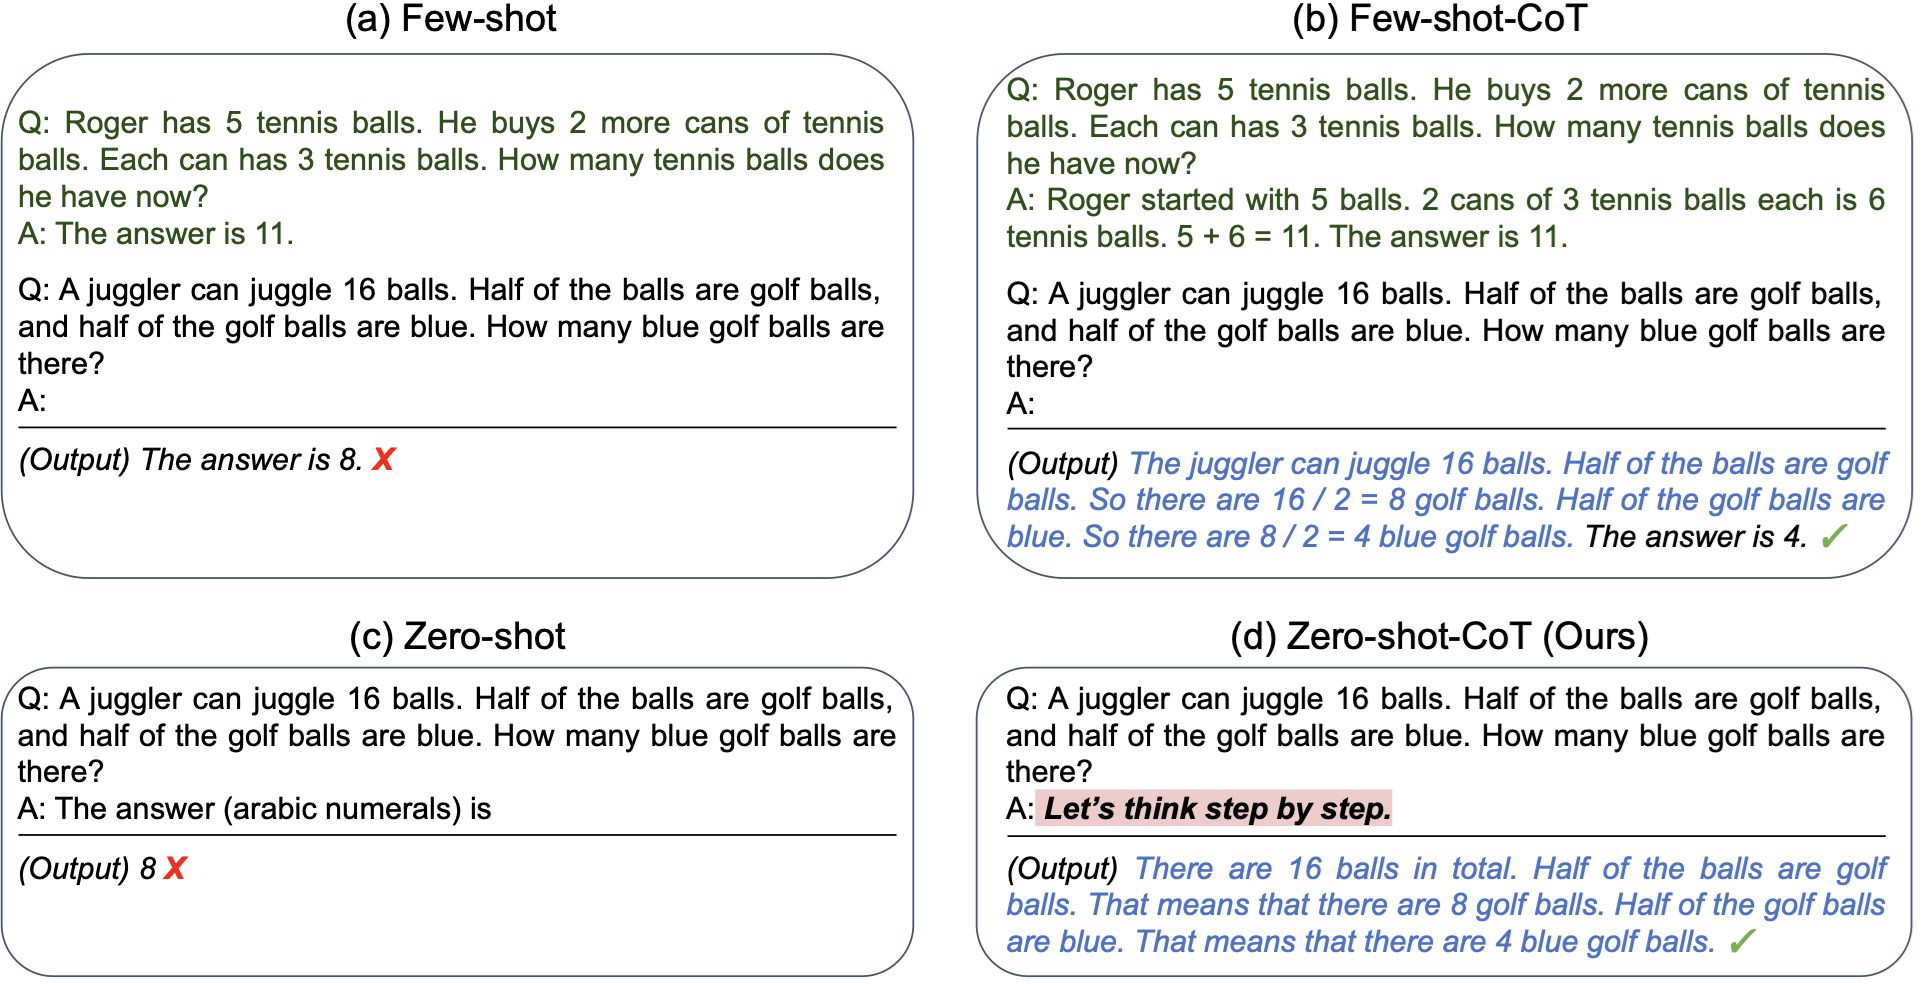
\includegraphics[width=0.9\textwidth]{./Figures/prompting.png}
	\caption{Ejemplo de uso de técnicas de \textit{prompting}.}
	\label{fig:prompting}
\end{figure}

A su vez, la ingeniería de \textit{prompts} ha demostrado ser fundamental en aquellos contextos en los que
el \textit{fine-tuning} no es viable, ya que hay muchos modelos cerrados que solo son accesibles a través de una API
y la capacidad de modificar su comportamiento sin reentrenamiento se vuelve crucial.
Por lo tanto, esta técnica se convierte en una herramienta práctica, eficiente y cada vez más sofisticada
para adaptar modelos generalistas a tareas específicas.

%----------------------------------------------------------------------------------------
%	SECTION 4
%----------------------------------------------------------------------------------------

\section{Ajuste fino}
El ajuste fino (\textit{fine-tuning}) \cite{howard2018universal} es una técnica de entrenamiento de modelos extensos de lenguaje 
que permite adaptar un modelo previamente entrenado a una tarea en específico.
A diferencia del entrenamiento desde cero, esta técnica parte de una base
y lo especializa utilizando un conjunto mucho más pequeño y específico de datos.
De este modo se reduce significativamente el coste computacional a la vez que se aprovecha
la capacidad predictiva del modelo del que se parte.

Para llevar a cabo el ajuste fino, se conservan la estructura y los parámetros previamente entrenados del modelo base,
evitando así la necesidad de un entrenamiento completo desde cero.
En la práctica, el proceso de \textit{fine-tuning} suele centrarse en modificar únicamente una parte reducida del modelo,
como las capas superiores, que son las más cercanas a la salida y, por tanto,
más fácilmente adaptables a tareas específicas.
Alternativamente, pueden integrarse nuevas capas que se entrenan sin alterar el resto del modelo.
Esta aproximación permite preservar los conocimientos generales adquiridos durante el preentrenamiento
mientras se optimiza la capacidad del modelo para tareas concretas.

Además, en escenarios con recursos computacionales limitados
se utilizan técnicas de ajuste fino eficiente (parameter-efficient fine-tuning, PEFT),
como LoRA (\textit{Low-Rank Adaptation}) \cite{hu2021lora},
\textit{prefix tuning} \cite{li2021prefix} o \textit{prompt tuning}.
Estas estrategias reducen la cantidad de parámetros que deben entrenarse,
lo que no solo disminuye el tiempo de ajuste y el consumo de memoria,
sino que también facilita la reutilización del modelo base en múltiples contextos sin interferencia entre tareas.

Al adaptar un modelo generalista a contextos específicos,
se logra una mejora sustancial en la precisión, relevancia y
sensibilidad del modelo frente a matices del lenguaje propios del área de aplicación.
No obstante, es fundamental contar con datos de alta calidad y
bien etiquetados para evitar la sobreespecialización o la introducción de sesgos.

\pagebreak
%----------------------------------------------------------------------------------------
%	SECTION 5
%----------------------------------------------------------------------------------------
\section{LM Studio y otras tecnologías}
LM Studio \cite{lmstudio} es una plataforma de código abierto diseñada para facilitar la interacción
y despliegue de modelos extensos de lenguaje (LLM) de manera local,
lo que permite a los usuarios ejecutar y experimentar con modelos sin depender de servicios en la nube.
Esta herramienta destaca por su integración sencilla, soporte para múltiples formatos de modelos y una interfaz amigable.

Una de las ventajas clave de LM Studio es su capacidad para manejar modelos grandes y complejos con eficiencia.
Ofrece funcionalidades como la gestión de memoria optimizada,
soporte para cuantización y carga progresiva de modelos
lo que permite que usuarios con recursos limitados puedan aprovechar la potencia de los LLM
sin necesidad de infraestructura costosa.
Además, LM Studio facilita la personalización de modelos mediante interfaces accesibles,
lo que la convierte en una opción popular tanto para investigadores como para desarrolladores
que desean incorporar inteligencia artificial avanzada en sus proyectos.

Para la implementación del \textit{backend} de la aplicación que interactúa con LM Studio, se utilizó \textit{Python},
un lenguaje de programación ampliamente adoptado en el ámbito de la inteligencia artificial por su simplicidad
y la gran cantidad de bibliotecas disponibles.
Se empleó la biblioteca de FastAPI \cite{fastapi} en al construcción del servidor web gracias a su sintaxis intuitiva,
lo que facilitó la creación de \textit{endpoints} eficientes para la comunicación entre el usuario y el modelo.

Por otro lado, \textit{PyTorch} \cite{pytorch} es la biblioteca de referencia para el desarrollo 
y entrenamiento de modelos de aprendizaje profundo, incluyendo los LLM.
Proporciona una interfaz dinámica y flexible que permite tanto el entrenamiento
como la inferencia eficiente en hardware acelerado, y es compatible con múltiples plataformas. 
	\chapter{Diseño e implementación} % Main chapter title
\label{Chapter3} % Change X to a consecutive number; for referencing this chapter elsewhere, use \ref{ChapterX}
En este capítulo se detalla cómo se ha ejecutado la implementación del trabajo,
incluyendo la arquitectura del sistema, procesamiento de peticiones,
modelos extensos de lenguaje utilizados y las técnicas empleadas sobre la inteligencia artificial.
Adicionalmente, se incluyen los hallazgos intermedios significativos que fueron fundamentales para la implementación final.

\definecolor{mygreen}{rgb}{0,0.6,0}
\definecolor{mygray}{rgb}{0.5,0.5,0.5}
\definecolor{mymauve}{rgb}{0.58,0,0.82}

%%%%%%%%%%%%%%%%%%%%%%%%%%%%%%%%%%%%%%%%%%%%%%%%%%%%%%%%%%%%%%%%%%%%%%%%%%%%%
% parámetros para configurar el formato del código en los entornos lstlisting
%%%%%%%%%%%%%%%%%%%%%%%%%%%%%%%%%%%%%%%%%%%%%%%%%%%%%%%%%%%%%%%%%%%%%%%%%%%%%
\lstset{ %
  backgroundcolor=\color{white},   % choose the background color; you must add \usepackage{color} or \usepackage{xcolor}
  basicstyle=\footnotesize,        % the size of the fonts that are used for the code
  breakatwhitespace=false,         % sets if automatic breaks should only happen at whitespace
  breaklines=true,                 % sets automatic line breaking
  captionpos=b,                    % sets the caption-position to bottom
  commentstyle=\color{mygreen},    % comment style
  deletekeywords={...},            % if you want to delete keywords from the given language
  %escapeinside={\%*}{*)},          % if you want to add LaTeX within your code
  %extendedchars=true,              % lets you use non-ASCII characters; for 8-bits encodings only, does not work with UTF-8
  %frame=single,	                % adds a frame around the code
  keepspaces=true,                 % keeps spaces in text, useful for keeping indentation of code (possibly needs columns=flexible)
  keywordstyle=\color{blue},       % keyword style
  language=[ANSI]C,                % the language of the code
  %otherkeywords={*,...},           % if you want to add more keywords to the set
  numbers=left,                    % where to put the line-numbers; possible values are (none, left, right)
  numbersep=5pt,                   % how far the line-numbers are from the code
  numberstyle=\tiny\color{mygray}, % the style that is used for the line-numbers
  rulecolor=\color{black},         % if not set, the frame-color may be changed on line-breaks within not-black text (e.g. comments (green here))
  showspaces=false,                % show spaces everywhere adding particular underscores; it overrides 'showstringspaces'
  showstringspaces=false,          % underline spaces within strings only
  showtabs=false,                  % show tabs within strings adding particular underscores
  stepnumber=1,                    % the step between two line-numbers. If it's 1, each line will be numbered
  stringstyle=\color{mymauve},     % string literal style
  tabsize=2,	                   % sets default tabsize to 2 spaces
  title=\lstname,                  % show the filename of files included with \lstinputlisting; also try caption instead of title
  morecomment=[s]{/*}{*/}
}


%----------------------------------------------------------------------------------------
%	SECTION 1
%----------------------------------------------------------------------------------------
\section{Arquitectura del sistema}

Los primeros esfuerzos en el desarrollo del trabajo se enfocaron en definir el conjunto de módulos que compondrían la solución.
Estos componentes fueron identificados correctamente desde el principio:
un servidor \textit{web} y un módulo de modelos extensos de lenguaje.
Sin embargo, su relación en el sistema sí cambió durante la fase de implementación.

Inicialmente, durante la fase de diseño, se concibió que el servidor \textit{web} también alojaría el modelo extenso de lenguaje 
y sería responsable de gestionar su conjunto de datos, entrenamiento y despliegue.
Esta decisión se tomó al principio de la implementación,
influenciada por la forma en la que se trabaja con redes neuronales sencillas.
Hacer que esa arquitectura funcionase en este trabajo era mucho más complejo de lo estimado
por la propia naturaleza de los modelos extensos de lenguaje.
La incertidumbre generada por la ausencia de un conjunto de datos de calidad y tamaño suficientes,
y la dificultad implícita de reentrenar un modelo tan grande,
fueron un factor de riesgo permanente durante la fase de diseño.

Fue necesario profundizar en las materias de procesamiento de lenguaje natural y \textit{Large Language Models} \cite{fiubaLlm}
para definir una solución efectiva a este problema.
Finalmente se decidió por no solo ``extraer'' el módulo de modelos extensos de lenguaje del servidor \textit{web}
sino por simplificar su complejidad de programación haciendo uso de la herramienta LM Studio.
Este programa permite administrar los modelos locales de la computadora,
añadir nuevos a través de una interfaz de descarga
y hacer uso del hardware disponible para arrancarlos de forma transparente para el usuario.
Además, cuenta con varias ventanas de configuración de parámetros de lanzamiento del modelo, \textit{prompts} personalizados,
salida estructurada a través de un esquema JSON,
opciones relacionadas con la aleatoriedad y temperatura de la inferencia y otras características experimentales.

De este modo, el servidor \textit{web} también se simplificó en el desarrollo, ahorró mucho trabajo de programación sin
comprometer la calidad del proceso de la inteligencia artificial.
Esto también es coherente con la arquitectura de servidor ligero esperable en un prototipo
y tiene una mejor sinergia con bibliotecas orientadas al despliegue de servidores sencillos.

Tal y como se muestra en la figura \ref{fig:sist},
el prototipo es accesible para los clientes a través del protocolo HTTP-REST que expone el servidor.
Además, durante el desarrollo se implementó una sencilla página \text{web} para realizar peticiones de prueba
y mostrar la salida de texto obtenida.

\begin{figure}[htbp]
	\centering
	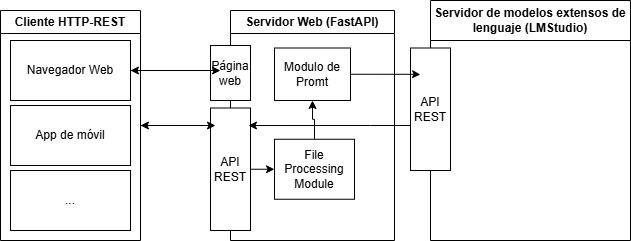
\includegraphics[width=0.9\textwidth]{./Figures/Sistema_es.png}
	\caption{Arquitectura del sistema.}
	\label{fig:sist}
\end{figure}

Otra ventaja de haber diseñado ambos módulos de forma independiente es que facilita al cliente
profundizar de forma paralela en los componentes sin comprometer el funcionamiento del resto del sistema.
Puede decidir si sustituir la implementación de uno u ambos módulos, escalarlos y distribuirlos en distintos entornos
para ajustarlo a su aplicación para \text{smartphones} y plan de expansión de servicios. 

%----------------------------------------------------------------------------------------
%	SECTION 2
%----------------------------------------------------------------------------------------
\section{Procesamiento de peticiones \textit{web} y ficheros}
Para la implementación del servidor web se decidió utilizar la biblioteca de FastAPI \cite{fastapi}.
Es una biblioteca moderna y de alto rendimiento para la construcción de APIs \text{web} en Python,
diseñada sobre estándares como OpenAPI \cite{openapi} y JSON schema.
Ofrece una forma rápida y eficiente de desarrollar interfaces REST
con una sintaxis sencilla y basada en anotaciones.
Esto permite una validación automática de datos de entrada y generación de documentación.
Todo esto hace que FastAPI sea una opción ideal para construir microservicios y prototipos rápidos.

El servidor expone dos servicios principales.
El primero es un \textit{endpoint} de tipo GET que proporciona la página \textit{web} que visualiza la interfaz gráfica del prototipo.
El otro servicio implementa un método POST para recibir las peticiones de consulta por parte del usuario para su procesamiento
y reenvío al módulo de inteligencia artificial. 


\pagebreak
\subsection{Procesamiento de peticiones}
En la figura \ref{fig:flux} se representa el diagrama de flujo correspondiente al manejo de las peticiones entrantes.

\begin{figure}[htbp]
	\centering
	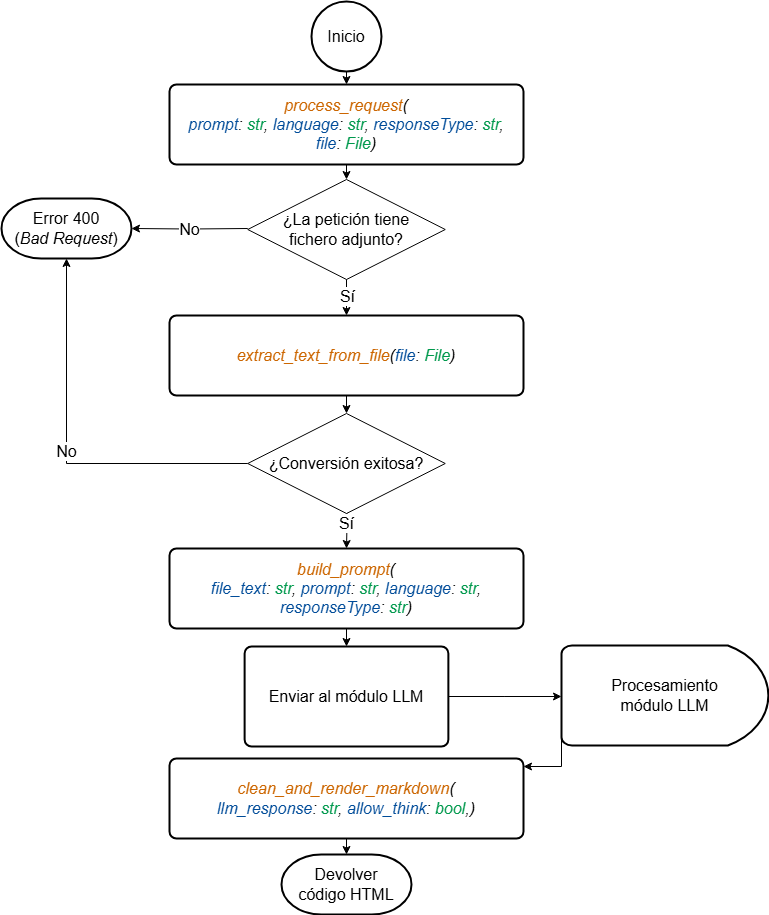
\includegraphics[width=1\textwidth]{./Figures/flux-diagram.png}
	\caption{Diagrama de flujo del procesamiento de peticiones.}
	\label{fig:flux}
\end{figure}

El proceso comienza cuando el cliente envía una solicitud con los datos de consulta a través de un cliente REST.
Esto puede ser a través del formulario proporcionado por el servidor o a través de cualquier otra herramienta como,
por ejemplo, PostMan.
Tras realizar las comprobaciones iniciales,
el servidor continúa procesando la información mediante una serie de funciones específicas:
\begin{itemize}
\item \texttt{extract\_text\_from\_file}:
es el proceso encargado de extraer la información textual de los ficheros adjunto
y formatearlo para que el módulo de modelos extensos de lenguaje sea capaz de interpretarlo.
En esta función se hace uso de las bibliotecas de cgardet, docx y fitz para la detección del formato y
su conversión a texto plano.
\item \texttt{build\_prompt}:
esta función es la encargada de construir el \textit{prompt} a partir del texto extraído del fichero
y las entradas adicionales proporcionadas por el usuario, entre las que se incluyen el idioma de
la respuesta, el tipo de listado que se solicita y algunas instrucciones adicionales.
En esta función se emplea la ingeniería de \textit{prompting} que se envía posteriormente al módulo LLM.
Se detalla más adelante en la sección \ref{subsec:prompt}.
\item \texttt{clean\_and\_render\_markdown}:
esta función se encarga de limpiar la salida y formatearla en código HTML
a través de la biblioteca markdown para una mejor legibilidad en navegadores web.
\end{itemize}

Cabe destacar que para la comunicación con el módulo LLM,
aunque LM Studio ofrece un SDK en Python para interactuar mediante programación,
se optó por utilizar su interfaz REST.
La razón es que así el servidor \textit{web} no depende exclusivamente de la biblioteca de LM Studio.
Al emplear un protocolo de comunicación estándar como REST,
el servidor web puede interactuar fácilmente con cualquier otro servicio que aloje modelos extensos de lenguaje,
lo que le da mayor flexibilidad.

\subsection{Interfaz gráfica}
El servidor también facilita el acceso a una página \textit{web} con la interfaz gráfica del prototipo,
tal y como se aprecia en la figura \ref{fig:webPage}.

\begin{figure}[htbp]
	\centering
	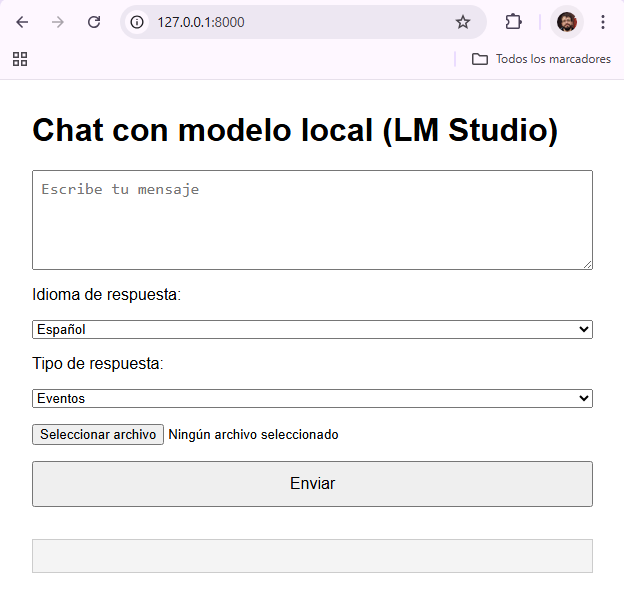
\includegraphics[width=0.8\textwidth]{./Figures/webpage.png}
	\caption{Interfaz gráfica del prototipo.}
	\label{fig:webPage}
\end{figure}

El formulario consta de los siguientes elementos:
\begin{itemize}
\item Cuadro de texto:
este elemento se utiliza para darle las instrucciones específicas a la inteligencia artificial.
Está pensado para que sea un mensaje breve y conciso que pueda ayudar al usuario a guiar un poco mejor la respuesta.
Es un parámetro opcional y puede dejarse en blanco.
\item Idioma de respuesta:
se trata de un \textit{combobox} que contiene dos opciones: inglés y español.
El módulo LLM responderá en el idioma seleccionado, independientemente del idioma del fichero de entrada.
Este elemento se añadió porque algunos modelos presentan comportamientos anómalos si responden en un idioma distinto al inglés.
\item Tipo de respuesta:
permite a la inteligencia artificial centrar su respuesta en un aspecto concreto de la narrativa.
Al estar instruida en devolver listas de elementos, la idea es que el usuario pueda elegir la opción
específica de la creación de mundos que le interese.
\item Fichero adjunto:
es el elemento más importante del formulario.
El usuario puede agregar un fichero con el contexto narrativo existente
y enviarlo a la inteligencia artificial para que genere nuevo contenido.
\end{itemize}

%----------------------------------------------------------------------------------------
%	SECTION 3
%----------------------------------------------------------------------------------------
\section{Gestión de modelos extensos de lenguaje}
El siguiente paso en la fase de implementación fue la instalación
y configuración del módulo de modelos extensos de lenguaje.
Inicialmente, se analizó si la gestión y comunicación con la LLM se haría a través de una
API en la nube o alojarlo localmente en el servidor \textit{web}.

La opción de la API implicaba depender de servicios externos
en internet, lo que resultaba en peores tiempos de respuesta y un coste adicional significativo
debido a los modelos de pago por uso que restringen la cantidad de consultas.
A su vez, la interacción con servicios externos exponía la información transmitida en las consultas
lo que podría incumplir los requerimientos de protección de la privacidad
y propiedad intelectual de los datos del cliente.
También se observó un menor número de modelos disponibles y opciones de personalización,
lo que dificultaba la experimentación y adaptación de los LLM a las necesidades específicas del sistema.

Por otra parte, la opción de gestionar los modelos extensos de lenguaje
de forma nativa presentaba desafíos considerables.
Desarrollar la infraestructura \textit{software} necesaria para la gestión de modelos
era una tarea con alta complejidad técnica que iba más allá de la mera integración de \textit{frameworks}.
Esto podía suponer limitaciones significativas en el proceso de configuración de los modelos y,
en consecuencia, provocar un coste elevado en términos de tiempo y recursos de desarrollo.

Por estos motivos se decidió buscar alternativas para este módulo y se encontraron varias herramientas que
cumplían con las características deseadas, y las más llamativas fueron
Ollama \cite{ollama}, GPT4All \cite{gpt4all} y LM Studio \cite{lmstudio}.
Esta última fue la opción elegida eventualmente por su interfaz intuitiva y buscador de modelos,
además de simplificar la gestión y configuración de los LLM.
Alojar localmente los modelos permite el envío ilimitado de consultas
y cumple con los requisitos de privacidad de los datos del cliente.

En los siguientes apartados se detallan los distintos procesos de gestión que se llevaron a cabo con LM Studio.

\subsection{Descarga de modelos}
El menú \textit{discover} de LM Studio da acceso al explorador de modelos extensos de lenguaje,
permitiendo a los usuarios navegar por una vasta biblioteca alojada principalmente en la plataforma Hugging Face \cite{huggingface}.
Como se ilustra en la figura \ref{fig:downloadMenu},
esta herramienta de búsqueda facilita la localización de modelos específicos mediante filtros por nombre o palabras clave,
presentando los resultados en un listado que se ajusta a los criterios definidos.
Al seleccionar un modelo, se muestra una sección de detalles con sus características y las distintas opciones de descarga disponibles.

\begin{figure}[htbp]
	\centering
	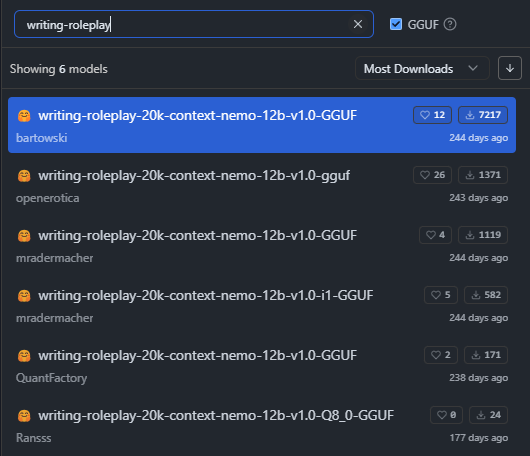
\includegraphics[width=0.8 \textwidth]{./Figures/download_menu.png}
	\caption{Buscador de modelos de LM Studio.}
	\label{fig:downloadMenu}
\end{figure}

Esta herramienta se empleó para la búsqueda y descarga de múltiples modelos,
que se enumeran y detallan en la subsección \ref{subsec:modelos-llm}.
Se eligieron tanto modelos generalistas como aquellos especializados en \textit{roleplay},
con el fin de analizar y comparar su rendimiento en tareas de construcción de mundos.

\subsection{Administración y configuración de modelos}
LM Studio permite la gestión y configuración de los modelos locales en el menú \textit{My Models}.
Además de listar los LLM descargados en el equipo, esta ventana permite personalizar
sus parámetros de ejecución para optimizar el rendimiento y la precisión de las respuestas.

\pagebreak
Como se muestra en la figura \ref{fig:configMenu},
al seleccionar un modelo se tiene acceso a un conjunto de ajustes agrupados
en varios conjuntos.
Como se trabajó en el \textit{prompting} en el servidor \textit{web},
los esfuerzos de configuración se centraron en los parámetros de carga e inferencia.

\begin{figure}[htbp]
	\centering
	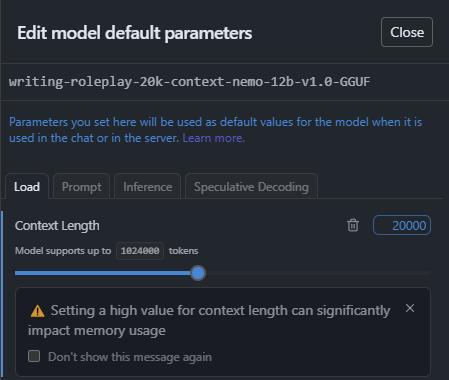
\includegraphics[width=0.8 \textwidth]{./Figures/config_menu.png}
	\caption{Configurador de modelos de LM Studio.}
	\label{fig:configMenu}
\end{figure}

La longitud del contexto resultó ser un parámetro fundamental en el trabajo.
Dado que las consultas de los usuarios se espera que vengan acompañadas de relatos extensos de \textit{worldbuilding},
era crucial que el LLM pudiera procesar y comprender grandes volúmenes de texto para generar respuestas coherentes y relevantes.
Los modelos tienen configurado por defecto un tamaño de contexto de 2048 o 4096 \textit{tokens},
un valor muy por debajo del tamaño de petición que se estima.

Para superar esta limitación, se seleccionó un tamaño de contexto compatible con las capacidades relativas de cada modelo,
a menudo indicado en los detalles.
Esta configuración fue esencial para asegurar que los LLM pudieran asimilar la totalidad de los relatos proporcionados.
Adicionalmente, se exploraron diversas tácticas para gestionar el exceso de contexto,
resultando más eficaces el acortamiento desde el principio de la secuencia o desde su punto medio.

Los parámetros de configuración de inferencia más importantes fueron la temperatura y
las técnicas de muestreo de probabilidad, como Top P o Top K.
Durante el desarrollo del proyecto, se observó que los valores predeterminados para estas variables
ya eran bastante adecuados. Por eso, solo fue necesario hacer ajustes mínimos en algunas de ellas.

Por defecto todos los modelos incluyen una sección de razonamiento.
Este parámetro fue deshabilitado en la configuración del modelo
y se filtró en el post-procesamiento para que no se mostrara en la respuesta al usuario.

\pagebreak
\subsection{Ejecución de modelos e interfaz REST}
La herramienta muestra y administra qué LLMs están activos y cargados en la memoria del sistema.
Además, también puede desplegar con un solo \textit{click} un servidor local compatible con la interfaz REST de OpenAI.
Cuando las peticiones llegan a este servidor, se registran en un log detallado que no solo proporciona
información sobre su estado sino que también muestra datos cruciales para la depuración de salidas incorrectas o errores.

\begin{figure}[htbp]
	\centering
	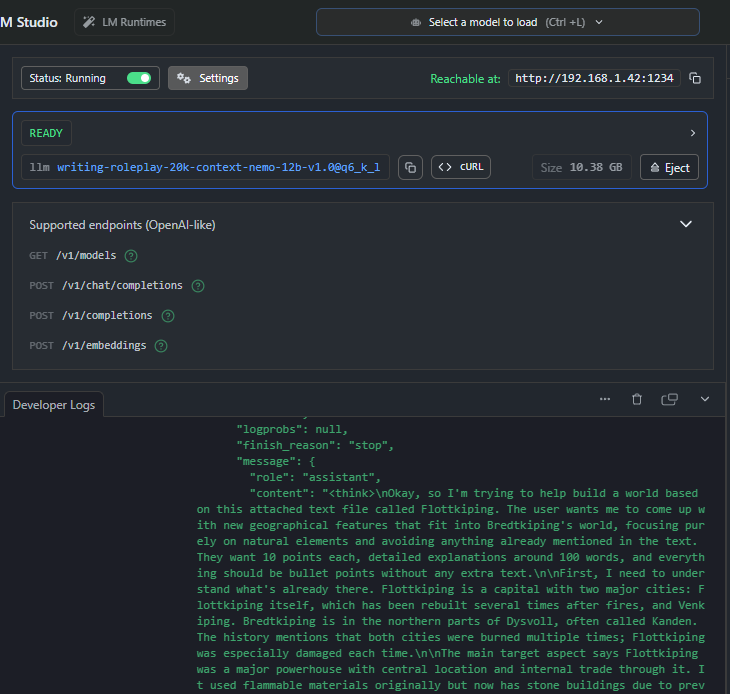
\includegraphics[width=1.0 \textwidth]{./Figures/developer_menu.png}
	\caption{Menú de desarrollador de LM Studio.}
	\label{fig:developerMenu}
\end{figure}

Una vez el modelo y el servidor están activos, el flujo del procesamiento de peticiones de la solución está completo.
El LLM, ya configurado con el tamaño de contexto ampliado y los parámetros de aleatoriedad ajustados,
gestiona la entrada, generando las respuestas esperadas.
Este diseño permite la misma forma de gestionar las peticiones,
sin importar el modelo que esté activo.

\pagebreak
\subsection{Modelos extensos de lenguaje utilizados}\label{subsec:modelos-llm}
El conjunto de modelos empleados en este trabajo se obtuvo a través de la herramienta de descarga de LM Studio.
Fueron seleccionados con un número de parámetros y un nivel de cuantización adecuado,
sin superar el límite de 12~GB de tamaño en memoria RAM dedicada en la tarjeta gráfica.
Esta parametrización permite aprovechar al máximo las capacidades del \textit{hardware} disponible,
con el objetivo de evaluar el rendimiento de distintos LLMs en tareas de generación narrativa.
En la tabla~\ref{tab:modelos_llm} se detallan las características de cada modelo:

\begin{table}[h]
\centering
\caption{Modelos extensos de lenguaje utilizados en el trabajo.}
\resizebox{\textwidth}{!}{%
\begin{tabular}{l l c c c r}
\toprule
\textbf{Modelo} & \textbf{Editor} & \textbf{Arquitectura} & \textbf{Parámetros} & \textbf{Cuantización} & \textbf{Tamaño (Contexto / VRAM)} \\
\midrule
\texttt{arliai-rpmax-v1.4} & bartowski & Mistral & 24 B & Q3\_K\_S & 20 k tokens / 10,40 GB \\
\texttt{writing-roleplay-v1.0} & bartowski & LLaMA & 12 B & Q6\_K\_L & 20 k tokens / 10,38 GB \\
\texttt{worldbuilder} & mrademacher & LLaMA & 12 B & Q6\_K & 4k tokens / 10,06 GB \\
\texttt{deepseek-r1-distill} & lmstudio & Qwen2 & 7 B & Q4\_K\_M & 32 k tokens / 4,68 GB \\
\texttt{mistral-instruct-v0.1} & TheBloke & Mistral & 8 B & Q8\_0 & 20 k tokens /  7,70 GB \\
\bottomrule
\end{tabular}%
}
\label{tab:modelos_llm}
\end{table}

Los tres primeros modelos referenciados fueron refinados específicamente para tareas de \textit{roleplay} y \textit{worldbuilding}.
Esto permite una mejor comprensión del fichero proporcionado por el usuario y una generación de contenido narrativo más coherente y contextualizado.

Con el fin de evaluar el rendimiento del sistema con las alternativas ampliamente accesibles en línea,
se incorporaron dos modelos generalistas que actúan como referencia.
Dado que estos modelos no han sido entrenados explícitamente para la creación narrativa,
la estrategia permite evaluar tanto la eficacia de la ingeniería de \textit{prompting} implementada,
como el impacto del entrenamiento específico en la capacidad de análisis del contexto y la calidad de las respuestas generadas.

%----------------------------------------------------------------------------------------
%	SECTION 4
%----------------------------------------------------------------------------------------
\section{Personalización del \textit{prompt} en función del servicio}

Una de las funcionalidades clave del sistema implementado consiste en la generación de la instrucción
a partir de la información proporcionada por el usuario en la petición.
Para guiar de forma efectiva la salida del modelo y obtener respuestas que cumplieran con los requerimientos del cliente,
se recurrió a diversas técnicas de ingeniería de \textit{prompting}.

\subsection{Función generadora de la instrucción}
\label{subsec:prompt}
Para aterrizar la lógica requerida se desarrolló en el módulo de \textit{prompt} la función \textit{build\_prompt}
y cuyo código se muestra debajo de este párrafo.
Este método se encarga de construir la instrucción alrededor del contexto narrativo,
extraído previamente del texto del fichero adjunto,
y combinarlo de forma estructurada con el resto de elementos de entrada.

\pagebreak
\begin{lstlisting}[label=cod:prompt,caption=Estructura de la función que construye la instrucción para el modelo.]
def build_prompt(file_text, additional_instructions, language, response_type):
    if response_type not in prompts:
        raise ValueError(
            f"Invalid output_type: '{response_type}'. Must be one of {list(prompts.keys())}"
        )

    general_prompt = prompts["general"]
    specific_prompt = prompts[response_type]

    content = (
        f"{general_prompt}\n"
        f"=== ATTACHED TEXT FILE ===\n"
        f"{file_text}\n\n"
        f"=== ADDITIONAL INSTRUCTIONS ===\n"
        f"{additional_instructions}"
        f"======\n"
        f"{specific_prompt}\n\n"
        f"Answer only in {language}.\n\n"
    )

    return {"role": "user", "content": content}

\end{lstlisting}

A continuación, se definen los elementos principales en orden secuencial:
\begin{itemize}
\item \textit{response\_type}:
tipo de salida esperada por parte del modelo.
Este parámetro selecciona el \textit{prompt} específico dentro del conjunto de \textit{prompts},
y si el valor proporcionado no se encuentra definido en dicho conjunto, se lanza una excepción.
\item \textit{general\_prompt}:
fragmento introductorio de la instrucción, común para todos los tipos de respuesta, que establece el rol
y las directrices principales que tiene que seguir el modelo.
\item \textit{specific\_prompt}:
instrucción particular asociada al tipo de respuesta especificado en \texttt{response\_type}.
Complementa a la instrucción principal añadiendo detalles o restricciones más concretas,
adaptadas a la tarea específica que debe realizar el modelo.
\item \textit{file\_text}:
contenido del archivo de entrada con el contexto narrativo sobre el cual se construye
la instrucción que es enviada al modelo.
\item \textit{additional\_instructions}:
conjunto de instrucciones adicionales proporcionadas por el usuario.
Estas indicaciones permiten personalizar o enriquecer el comportamiento del modelo
y ajustar la respuesta a necesidades específicas.
\item \textit{language}:
idioma en el que debe responder el modelo.
Esta indicación se incluye al final del mensaje para garantizar que
la salida esté redactada exclusivamente en el idioma solicitado.
\end{itemize}

Esta implementación permite personalizar la instrucción de manera precisa según la categoría de respuesta
y otras variables contextuales.
Gracias a este enfoque basado en la técnica de \textit{prompt chaining},
se reduce significativamente la complejidad de la interacción entre el usuario y el modelo de lenguaje.
Además, garantiza una respuesta precisa sin necesidad de que el usuario, 
que previsiblemente utilizará el servicio desde un dispositivo con pantalla reducida,
posea conocimientos en ingeniería de \textit{prompting}.

\subsection{Refinado iterativo de las instrucciones}
Una vez se definió la estructura general del mensaje, el siguiente paso consistió en optimizar tanto la instrucción general
como las indicaciones específicas asociadas a cada elemento de la ambientación narrativa. 
Este proceso fue esencial para garantizar que las respuestas generadas por los modelos se alinearan con las
expectativas propias de un asistente creativo que proporcionara listas de nuevas ideas.

El refinamiento se llevó a cabo de forma iterativa, como se muestra en la figura \ref{fig:iterativeRefinement},
a través de prueba y error con múltiples variantes para las instrucciones.
En cada ciclo se evaluaron las respuestas del modelo en función tanto de la estructura del contenido como de su coherencia
con el contexto narrativo aportado.
Esto permitió identificar errores en la formulación del \textit{prompt} responsables de alucinaciones,
repeticiones de información y otras inconsistencias en la generación de texto de los modelos.
En función del reto encontrado, se analizó la forma de solucionarlo mediante el empleo de técnicas
entre las que se encuentran \textit{chain of thought}, \textit{instruction-based prompting},
\textit{constrained-output prompting} y \textit{negative prompting}.

\begin{figure}[htbp]
	\centering
	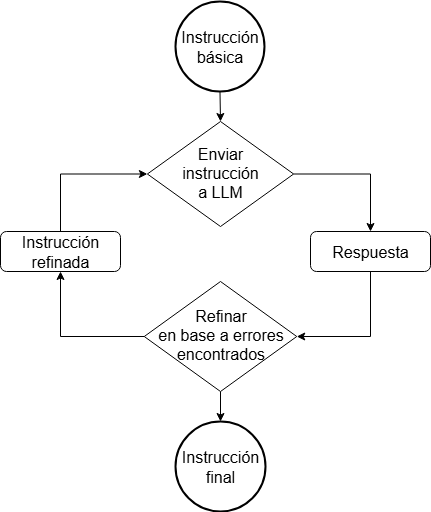
\includegraphics[width=0.7 \textwidth]{./Figures/iterative-process.png}
	\caption{Proceso de refinamiento de instrucciones.}
	\label{fig:iterativeRefinement}
\end{figure}

\pagebreak
En estre proceso se trabajó sobre cinco instrucciones diferentes:
\begin{itemize}
\item General:
se centró en resolver los problemas comunes detectados en todas las categorías narrativas.
En versiones iniciales, el modelo no generaba listas de forma adecuada ni mantenía un formato consistente en la respuesta.
También mostró dificultades para distinguir entre el contexto narrativo y las instrucciones que debía seguir.
Esto derivaba en repeticiones de información ya presentes en el texto de referencia, lo que limitaba considerablemente
la originalidad y riqueza de sus propuestas.
Por estas razones, fue necesario reformular la instrucción 
mediante la incorporación de directrices explícitas sobre el objetivo del modelo,
el formato de salida y la distinción entre contexto e instrucciones.
Se establecieron requisitos claros sobre la longitud mínima de las listas,
el nivel de detalle esperado en cada punto
y la obligatoriedad de que todos los elementos fueran completamente nuevos.
\item Eventos:
se enfocó en guiar al modelo
hacia la generación de sucesos nuevos que enriquecieran el desarrollo del mundo narrativo
sin duplicar hechos ya mencionados en el texto base.
En versiones preliminares, el modelo tendía a reformular eventos existentes en lugar de inventar situaciones originales.
Esto es debido al fuerte entrenamiento de los modelos a no modificar hechos que se consideran históricos.
Para resolver esto, se eliminó la palabra ``histórico'' de la instrucción y
se reforzó la indicación de que los eventos debían ser completamente inéditos
y conectados de forma coherente con el contexto.
\item Personajes:
las versiones iniciales del \textit{prompt} no ofrecían suficientes indicaciones estructurales,
lo que resultaba en respuestas incompletas o poco claras.
Algunos personajes carecían de nombre, contexto o motivación dentro del mundo ficticio.
Para solventar esto, la instrucción fue reescrita para exigir explícitamente un nombre, apellido,
alias (si procede) y una explicación clara de la relación del personaje con la historia o el entorno.
\item Geografía:
fue afinada para evitar confusiones entre elementos naturales y construcciones humanas.
En iteraciones anteriores, el modelo a menudo mezclaba ríos o montañas con ciudades o estructuras artificiales,
y no siempre justificaba la relevancia geográfica de los elementos descritos.
Para corregir esto, se incorporó una aclaración sobre el tipo de elementos geográficos aceptados
y se exigió una descripción detallada de cada punto, así como su importancia ecológica,
simbólica o estratégica dentro del mundo narrativo.
\item Localizaciones:
buscó mejorar la claridad y especificidad de los núcleos poblacionales propuestos.
En las versiones previas, el modelo a menudo confundía localizaciones con elementos geográficos
o entregaba descripciones genéricas sin conexión con el resto del mundo,
al utilizar la palabra ``asentamientos'' hubo una mejoría notable en el rendimiento.
La nueva versión de la instrucción estableció que debían generarse únicamente poblaciones (ciudades, pueblos, países)
y que cada una debía incluir una descripción detallada de sus características culturales, políticas o históricas,
así como su función o importancia dentro del contexto narrativo.
\end{itemize}

\pagebreak
En este proceso se utilizaron diversos corpus como contexto
con el objetivo de contrastar el comportamiento de los modelos en distintas situaciones.
A modo de anécdota, uno de los textos empleados estaba ambientado en una franquicia conocida
y los LLM generaron respuestas que incluían información propia de ese universo,
a pesar de no estar explícitamente presente en el texto proporcionado.
Esto sugiere que fueron entrenados previamente con contenidos relacionados con dicha ambientación.

Se puede consultar la versión final de las instrucciones desarrolladas en este trabajo en el Anexo (FALTA REFERENCIA).
Dado que el inglés es el idioma preferente de los modelos,
las instrucciones se redactaron en ese idioma.
Por esto mismo, se incluye una instrucción final para que la respuesta se genere en el idioma seleccionado por el usuario.
Sin embargo, es importante señalar que no todos los modelos soportan el español,
lo que ocasionalmente lleva a que esta última instrucción sea ignorada.
Este fenómeno se detallará en la siguiente sección.
	% Chapter Template

\chapter{Ensayos y resultados} % Main chapter title

\label{Chapter4} % Change X to a consecutive number; for referencing this chapter elsewhere, use \ref{ChapterX}
En este capítulo se describe el conjunto de ensayos realizados sobre el sistema y se recopilan sus resultados.
Con este propósito, se explican las características del \textit{hardware} y el banco de pruebas que se emplearon.
Además, se explican los criterios de evaluación para determinar la calidad de las respuestas de los
modelos extensos de lenguaje.
Finalmente, se hace un análisis global de los resultados, destacando el grado de mejora que ofrece el sistema, así como
sus errores más comunes.

%----------------------------------------------------------------------------------------
%	SECTION 1
%----------------------------------------------------------------------------------------

\section{Entorno y banco de pruebas}
Los ensayos fueron ejecutados en un equipo de altas prestaciones, orientado a tareas de cómputo intensivo y procesamiento de modelos de lenguaje de gran tamaño.
Sus especificaciones son las siguientes:
\begin{itemize}
\item Memoria RAM: 64 GB.
\item Tarjeta gráfica: NVIDIA GeForce RTX4080 SUPER, con 16 GB de memoria RAM dedicada.
\item Procesador: AMD Ryzen9 7950X3D 16-Core.
\item Sistema Operativo: Windows 11.
\end{itemize}

Aunque se emplearon diversos \textit{worldbuildings} en el proceso iterativo de refinamiento de las instrucciones,
el contexto narrativo de prueba se basó exclusivamente en textos pertenecientes al mundo de ficción ``Aanrah'',
desarrollado por el autor Necrowmancer en la plataforma de WorldAnvil \cite{aanrah2024}.
Esta ambientación fue seleccionada por ofrecer una combinación equilibrada de complejidad conceptual,
léxico específico y coherencia interna, sin alcanzar un volumen excesivo de contenido.
Dicha elección refleja el tipo de entradas que previsiblemente introducirán los usuarios del sistema,
al tiempo que plantea un desafío suficientemente realista para los modelos extensos de lenguaje.
El corpus de referencia se encuentra detallado en el apéndice \ref{AppendixB}.

%----------------------------------------------------------------------------------------
%	SECTION 2
%----------------------------------------------------------------------------------------

\section{Pruebas de procesamiento de ficheros}
Para comprobar el funcionamiento del procesamiento de los ficheros sin depender del módulo de procesamiento de peticiones \textit{web},
se implementaron varias celdas en un \textit{notebook} de Jupyter.
Esta solución no solo permite evaluar de forma controlada el comportamiento del módulo,
sino que además cumple con los criterios de pruebas automatizadas exigidos por el cliente.

Además, se formateó el contexto narrativo de prueba en los tres tipos de fichero aceptados: txt, docx y pdf.
El funcionamiento del módulo quedó validado tras comprobar que el texto extraído de todos los ficheros es idéntico,
tal y como se muestra en las figuras \ref{fig:txt-read-test}, \ref{fig:docx-read-test} y \ref{fig:pdf-read-test}.
Se aprecian diferencias de formato en el archivo pdf, pero su contenido coincide.

\begin{figure}[htbp]
	\centering
	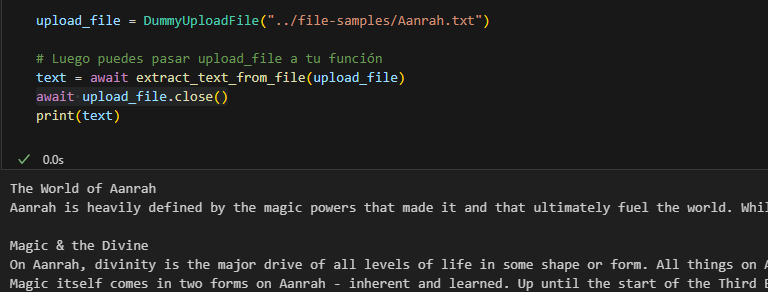
\includegraphics[width=0.9\textwidth]{./Figures/file-read-test-txt.png}
	\caption{Prueba de lectura de ficheros txt.}
	\label{fig:txt-read-test}
\end{figure}

\begin{figure}[htbp]
	\centering
	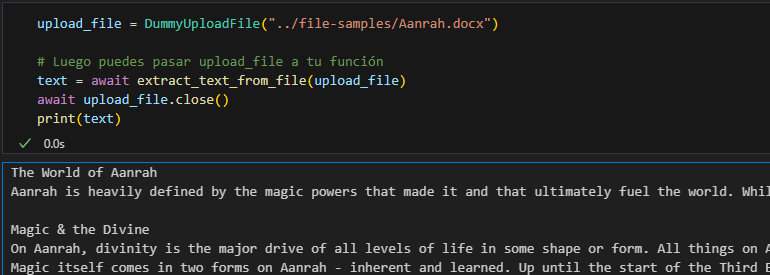
\includegraphics[width=0.9\textwidth]{./Figures/file-read-test-docx.png}
	\caption{Prueba de lectura de ficheros docx.}
	\label{fig:docx-read-test}
\end{figure}

\begin{figure}[htbp]
	\centering
	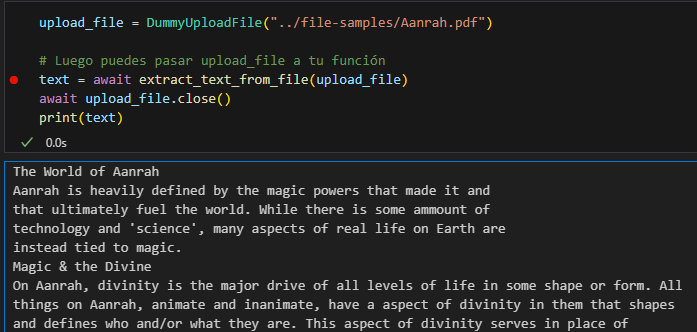
\includegraphics[width=0.9\textwidth]{./Figures/file-read-test-pdf.png}
	\caption{Prueba de lectura de ficheros pdf.}
	\label{fig:pdf-read-test}
\end{figure}

%----------------------------------------------------------------------------------------
%	SECTION 3
%----------------------------------------------------------------------------------------
\pagebreak
\section{Pruebas de procesamiento de peticiones web}
Durante la fase de implementación se llevaron a cabo pruebas incrementales que incluyeron
la verificación de la correcta carga del HTML, la recepción de las peticiones junto con los archivos adjuntos,
la lectura del contenido y, finalmente,
la integración completa del flujo de comunicación entre el usuario y el modelo extenso de lenguaje.
Cuando una petición se procesa correctamente, la información se envía de vuelta a la interfaz \textit{web},
donde se muestra en un cuadro de texto.

En la figura~\ref{fig:web-test} se muestra el resultado de una petición en la que,
con fines de prueba, se omitió el envío al módulo LLM
y en su lugar se devolvió directamente al usuario el contenido del fichero adjunto.

\begin{figure}[htbp]
	\centering
	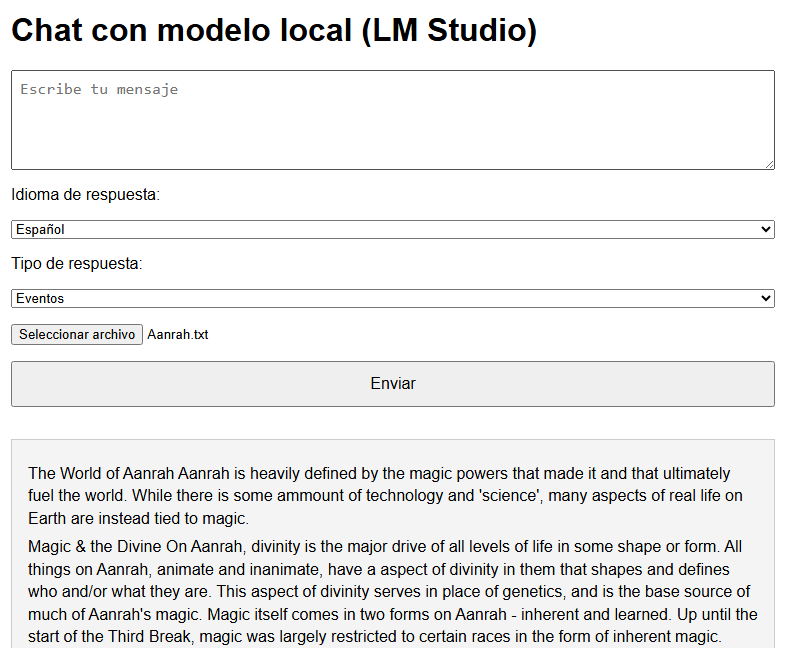
\includegraphics[width=1\textwidth]{./Figures/web-test.png}
	\caption{Prueba de envío de peticiones REST.}
	\label{fig:web-test}
\end{figure}

En las pruebas de los siguientes apartados se muestran múltiples figuras de la interfaz con el flujo completo de datos.

%----------------------------------------------------------------------------------------
%	SECTION 4
%----------------------------------------------------------------------------------------
\section{Método para valorar la salida de los modelos extensos de lenguaje}
En este apartado se explica la lógica que se siguió para valorar la calidad de las respuestas
generadas por el modelo de lenguaje.
Este proceso presenta una dificultad inherente:
debido a la naturaleza de los casos de uso del sistema, esta puntuación es completamente subjetiva.
Conceptos como “adecuación”, “originalidad” o “interés narrativo” no pueden medirse de forma objetiva ni automática,
lo que limita la posibilidad de una evaluación completamente reproducible.
Por ello, la validación fue realizada de forma manual, basándose en mi propio criterio como desarrollador del sistema.

Una vez aclarado este aspecto, las pruebas se estructuraron de forma que pudieran reproducirse de manera sencilla y sistemática.
En todas las evaluaciones se emplea el mismo fichero adjunto, que contiene el contexto narrativo base,
y se combina con cada tipo de elemento de \textit{worldbuilding} que se desea generar.
Este enfoque se aplica de forma consistente a todos los modelos extensos de lenguaje.
Adicionalmente, sobre este mismo conjunto de pruebas se compararán dos escenarios:
uno en el que se utiliza la ingeniería de \textit{prompting} desarrollada en este trabajo,
y otro en el que dicha técnica no se aplica.
Este contraste permitirá evaluar el impacto real de las instrucciones
refinadas sobre los modelos.

Para valorar la salida del modelo se emplearon los siguientes criterios:
\begin{itemize}
\item \textbf{Adecuación contextual}: se verifica que los elementos generados respeten el tono, estilo y detalles del contexto narrativo original.
\item \textbf{Pertinencia temática}: los resultados deben estar alineados con la categoría seleccionada
(por ejemplo, si se ha elegido ``personajes'', la salida no debe incluir ubicaciones o eventos).
\item \textbf{Originalidad}: se valora la capacidad del modelo para proponer ideas nuevas sin repetir explícitamente el contenido del fichero.
\item \textbf{Diversidad}: se analiza si la lista contiene variedad en las propuestas y evita repeticiones o elementos demasiado similares.
\item \textbf{Idioma}: se indica si el modelo acepta texto en español. 
\item \textbf{Consistencia}: analiza la inestabilidad en la respuesta de los modelos,
teniendo en cuenta que todos fueron configurados con una temperatura de 0,7 sobre 1. 
\item \textbf{Errores}: se listan los errores encontrados en las pruebas y se analiza el impacto que tienen.
\end{itemize}

%----------------------------------------------------------------------------------------
%	SECTION 5
%----------------------------------------------------------------------------------------
\section{Pruebas con modelos generalistas y \textit{prompting} poco preciso}
Esta sección analiza el rendimiento de los modelos que no han sido ajustados específicamente
para tareas de ambientación narrativa y que carecen de un refinamiento adecuado en las instrucciones.
El objetivo es simular los resultados que podrían obtenerse si una persona sin experiencia en ingeniería de
\textit{prompting} utilizara las opciones más comunes disponibles en línea.

Para lograr esto, se desactivó el módulo de \textit{prompts} y se bloquearon algunos controles de la interfaz
\textit{web} para que solo aceptara el fichero adjunto, el cuadro de texto y el selector de idiomas.
En la figura \ref{fig:prompt-test} se muestra
cómo el modelo responde libremente a la entrada del usuario.
Una vez validada la funcionalidad, todas las instrucciones se simplificaron en una única frase:
``dame una lista de diez nuevos'' seguido del elemento narrativo que se quería obtener.
\pagebreak
\begin{figure}[htbp]
	\centering
	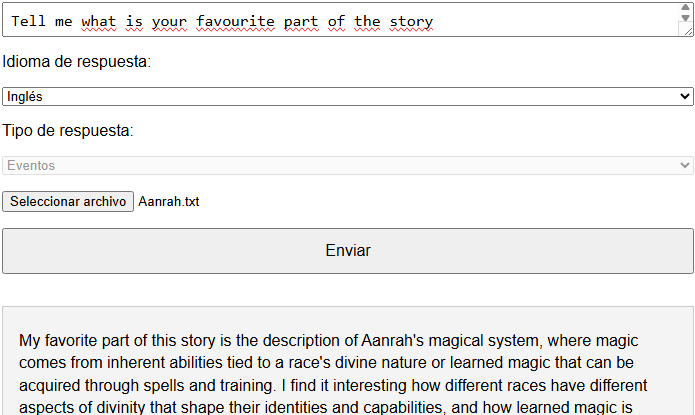
\includegraphics[width=1\textwidth]{./Figures/promp-testing.png}
	\caption{Prueba de desconexión del módulo generador de instrucciones.}
	\label{fig:prompt-test}
\end{figure}

\subsection{Resultados de \textit{deepseek}}
En el caso de \textit{deepseek}, presentó una adaptación al contexto narrativo aceptable y se ciñó correctamente al
tipo de elemento narrativo que se especificó.
No obstante, su desempeño en relación con la variedad de las ideas fue bajo al presentar puntos muy similares entre sí.
Este problema fue especialmente notable en el caso de los personajes y eventos.
Por último, la consistencia de sus respuestas varió en ocasiones.
Esto significa que su sensibilidad a la temperatura es bastante alta.
El modelo puede responder en español, pero los errores de traducción y alucinaciones son frecuentes,
tal y como se muestra en la figura \ref{fig:deepseek-esp}:

\begin{figure}[htbp]
	\centering
	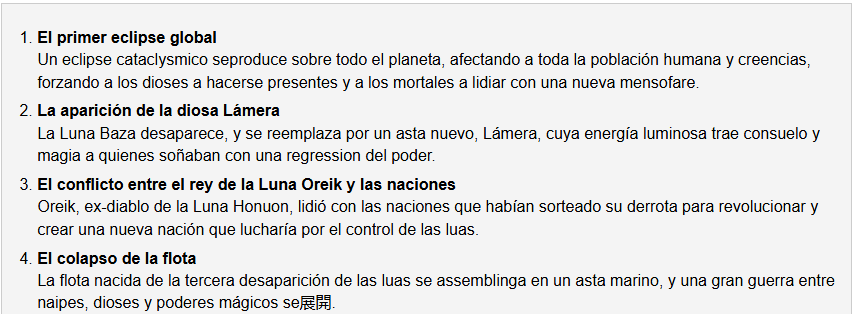
\includegraphics[width=1\textwidth]{./Figures/deepseek-noprompt-spanish.png}
	\caption{Resultado en español de \textit{deepseek} para eventos.}
	\label{fig:deepseek-esp}
\end{figure}
\pagebreak
\subsection{Resultados de \textit{mistral}}
El modelo generalista de \textit{mistral} no consiguió la misma calidad en sus respuestas.
Las propuestas, aunque tienen relación con el contexto de la historia,
muestran una conexión sin demasiada profundidad en los detalles ni en su variedad.
En los casos de geografía y asentamientos, su relación con el contexto es mínima o nula
(ver figura \ref{fig:mistral-geo}), lo que sugiere que su entrenamiento no le permite ser
flexible en la generación de contenido narrativo sin instrucciones previas.
Este modelo pierde completamente el contexto al responder en español,
lo que provoca que utilice referencias reales,
como ciudades de Estados Unidos, personajes históricos o festividades internacionales.

\begin{figure}[htbp]
	\centering
	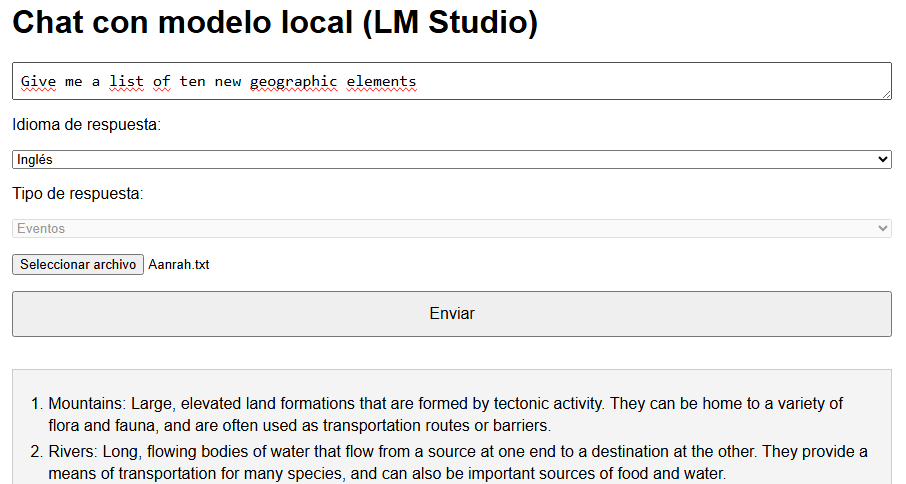
\includegraphics[width=1\textwidth]{./Figures/mistral-noprompt-geography.png}
	\caption{Resultado de \textit{mistral} para geografía}
	\label{fig:mistral-geo}
\end{figure}

%----------------------------------------------------------------------------------------
%	SECTION 6
%----------------------------------------------------------------------------------------
\section{Pruebas con modelos reentrenados y \textit{prompting} poco preciso}
Análogamente a la sección anterior, se llevaron a cabo pruebas equivalentes
sobre los modelos refinados con el fin de evaluar su rendimiento.
Los resultados permiten establecer una comparación entre estos LLM
y los modelos generalistas.

\subsection{Resultados de \textit{writing-roleplay}}
El modelo de \textit{writing-roleplay} funcionó correctamente en la generación de eventos,
comprendiendo adecuadamente el contexto y ofreciendo ideas interesantes.
Sin embargo, presentó problemas en el resto de elementos narrativos.
A pesar de que aporta una variedad aceptable y una ambientación de fantasía correcta,
su respuesta se ajusta más a un contenido predefinido que a algo adaptado a la ambientación
narrativa del fichero adjunto.
Finalmente, fue notoria la inconsistencia del modelo a la temperatura a la que fue configurado,
ya que ocasionalmente repetía información en vez de aportar ideas nuevas.

\subsection{Resultados de \textit{worldbuilder}}
En el caso de \textit{worldbuilder},
su comprensión de la entrada destacó sobre las alternativas generalistas,
aportando ideas con una relación profunda con el contexto de entrada
(Figura \ref{fig:worldbuilder-settle}).
Sin embargo, el modelo también tiene una sensibilidad alta a la temperatura
y ocasionalmente puede ignorar la ambientación al generar nuevo contenido.
Algo único de este LLM es que puede llegar a dar consejos al usuario de cómo
hacer la construcción de mundos, con diversas técnicas y explicaciones,
en vez de dar una lista de nuevas ideas.
También es el único que no puede dar respuestas en español.

\begin{figure}[htbp]
	\centering
	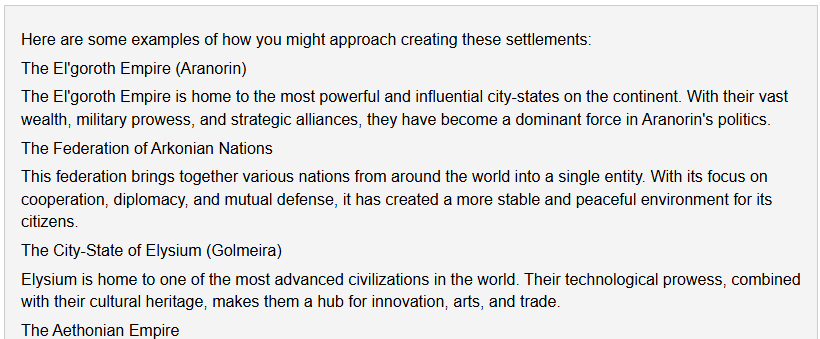
\includegraphics[width=1\textwidth]{./Figures/worldbuilder-noprompt-settlements.png}
	\caption{Resultado de \textit{worldbuilder} para asentamientos}
	\label{fig:worldbuilder-settle}
\end{figure}

\subsection{Resultados de \textit{arliai-rpmax}}
Finalmente, el modelo \textit{arliai-rpmax} fue el que mejor desempeño demostró. 
Se ajustó al contexto de entrada y profundizó en las respuestas de forma aceptable.
Donde también destacó es en la capacidad de generar texto en español sin verse afectado
en la calidad del mensaje. 

A nivel global, todos los LLM funcionaron bien para los eventos y las localizaciones,
mientras que carecieron de originalidad en la generación de personajes y geografía.
En la figura \ref{fig:rpmax-chars} se muestra un ejemplo de este fenómeno.

\begin{figure}[htbp]
	\centering
	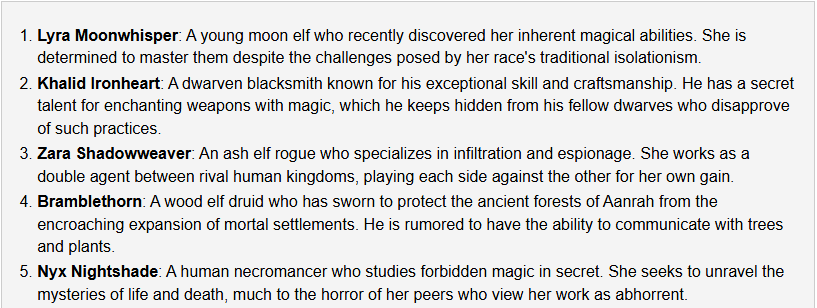
\includegraphics[width=1\textwidth]{./Figures/rpmax-noprompt-chars.png}
	\caption{Resultado de \textit{arliai-rpmax} para personajes}
	\label{fig:rpmax-chars}
\end{figure}

%----------------------------------------------------------------------------------------
%	SECTION 7
%----------------------------------------------------------------------------------------
\section{Pruebas con modelos generalistas y \textit{prompting} preciso}
Esta sección examina el rendimiento de modelos generalistas que no han sido específicamente
ajustados para tareas de ambientación narrativa.
A diferencia de enfoques anteriores sin refinamiento,
el objetivo aquí es maximizar la capacidad intrínseca del modelo mediante instrucciones detalladas,
buscando determinar la eficacia de esta técnica al trabajar con modelos accesibles públicamente.

Para ello, se hace uso del módulo de instrucciones y la interfaz \textit{web}
en su versión final. Tal y como se demuestra en la figura \ref{fig:full-prompt-test},
el sistema construye la instrucción de forma transparente para el usuario, por lo que
solo es necesario que se adjunte el fichero con el contexto narrativo.

\begin{figure}[htbp]
	\centering
	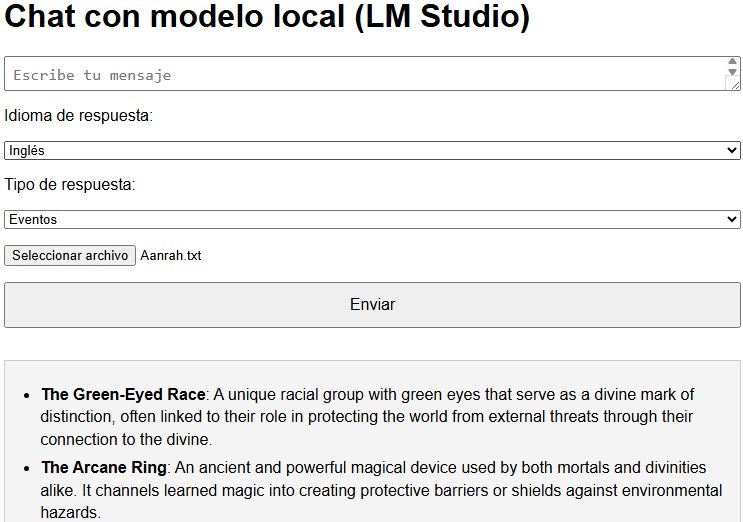
\includegraphics[width=0.85\textwidth]{./Figures/full-promp-testing.png}
	\caption{Prueba de la versión definitiva del sistema.}
	\label{fig:full-prompt-test}
\end{figure}

\subsection{Resultados de \textit{deepseek}}
Este modelo experimentó una mejora sustancial en la calidad de sus respuestas, tanto en la profundidad
contextual como en la variedad de las ideas que aporta.
La capacidad del modelo para relacionar elementos de la ambientación narrativa y
plasmarlos en las propuestas se vio significativamente potenciada, abarcando eventos, personajes y geografía
(ver figura \ref{fig:deepseek-prompt-char}).
La consistencia de las respuestas se mantuvo estable,
reduciéndose notablemente la aparición de errores de formato y temática.
Asimismo, el rendimiento en español mejoró, reduciendo el coste de la traducción.

\begin{figure}[htbp]
	\centering
	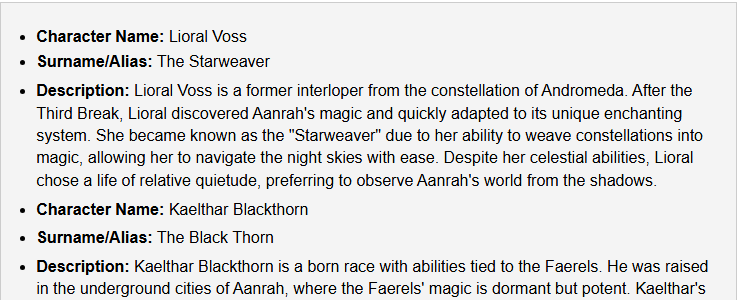
\includegraphics[width=1\textwidth]{./Figures/deepseek-prompt-characters.png}
	\caption{Resultado de \textit{deepseek} para personajes.}
	\label{fig:deepseek-prompt-char}
\end{figure}
\pagebreak
\subsection{Resultados de \textit{mistral}}
\textit{Mistral} mostró una adaptación inconsistente a la ingeniería de instrucciones precisas,
lo que se tradujo en una alta variabilidad en sus respuestas.
Aunque en algunos casos interpretó correctamente las directrices,
mostrando una ligera mejora respecto a las instrucciones básicas,
los errores fueron frecuentes. Entre los más comunes se incluyen la duplicación de la lista generada y
una pérdida considerable de la temática en la respuesta. Esto a menudo resultaba en la generación de más de los 10 elementos especificados por defecto,
con una relación mínima o nula con el contexto general.
Además, el modelo perdió por completo su capacidad de generar respuestas en español bajo esta configuración.

\begin{figure}[htbp]
	\centering
	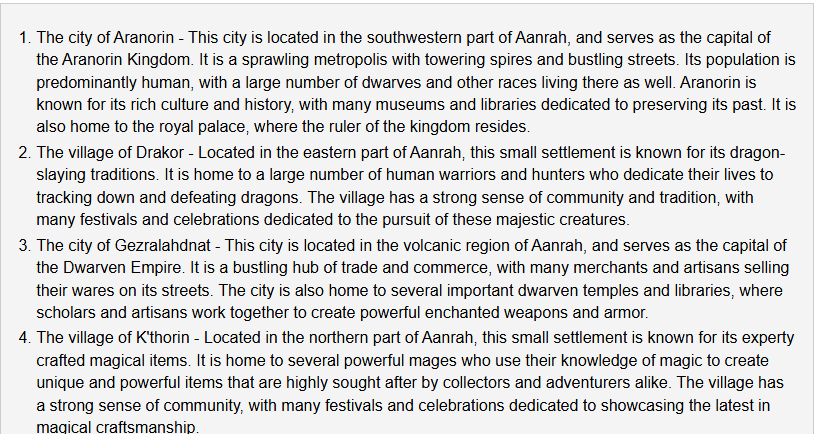
\includegraphics[width=1\textwidth]{./Figures/mistral-prompt-locations.png}
	\caption{Resultado de \textit{mistral} para localizaciones.}
	\label{fig:mistral-prompt-locations}
\end{figure}

%----------------------------------------------------------------------------------------
%	SECTION 8
%----------------------------------------------------------------------------------------
\section{Pruebas con modelos reentrenados y \textit{prompting} preciso}
Esta sección presenta y analiza los resultados obtenidos de las pruebas realizadas sobre los modelos refinados,
empleando esta vez instrucciones precisas.

\subsection{Resultados de \textit{writing-roleplay}}
La comprensión del LLM experimentó una ligera mejora,
siendo esta más evidente en la generación de eventos.
Sin embargo, en el resto de categorías, el rendimiento se mantuvo similar al observado con \textit{prompting} poco preciso.
En varias ocasiones, el modelo interpretó que debía generar una lista de varias decenas de puntos,
lo que provocó bloqueos en el sistema, indicando una posible sobrecarga o un fallo en el manejo de la longitud de la respuesta esperada.

\begin{figure}[htbp]
	\centering
	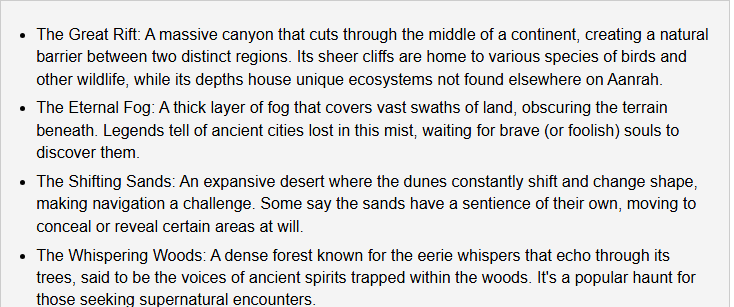
\includegraphics[width=1\textwidth]{./Figures/writing-prompt-geography.png}
	\caption{Alucinación de \textit{writing-roleplay} para geografía.}
	\label{fig:writing-geography}
\end{figure}

\subsection{Resultados de \textit{worldbuilder}}
Con la aplicación de las nuevas instrucciones, el modelo mostró
una mejora perceptible en la comprensión del contexto de entrada,
lo cual se reflejó en la calidad de la generación.
No obstante, en los apartados de geografía y localizaciones, no se observó una mejora significativa.
En esta configuración, también se registraron alucinaciones, como se ilustra en la figura \ref{fig:worldbuilder-hallucination},
que complejizaron el listado y llevaron a la devolución de varias listas con diferentes categorías,
sugiriendo nuevamente una tendencia a desviarse de la estructura de respuesta esperada.

\begin{figure}[htbp]
	\centering
	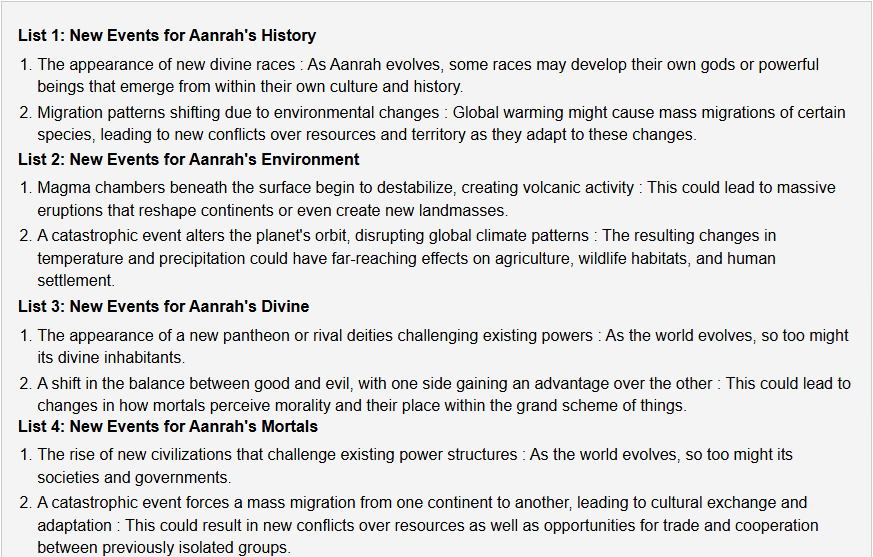
\includegraphics[width=1\textwidth]{./Figures/worldbuilder-hallucination-events.png}
	\caption{Alucinación de \textit{worldbuilder} en la generación de eventos.}
	\label{fig:worldbuilder-hallucination}
\end{figure}

\subsection{Resultados de \textit{arliai-rpmax}}
Gracias al refinamiento de los \textit{prompts},
este modelo mejoró significativamente su comprensión e inclusión del contexto,
lo que resultó en respuestas de calidad excepcional.
Además, \textit{arliai-rpmax} destacó por su robusta capacidad de generar texto en español,
manteniendo una calidad constante en el mensaje sin degradación.

\begin{figure}[htbp]
	\centering
	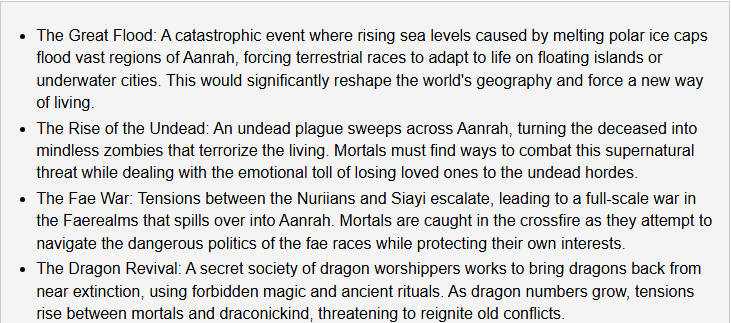
\includegraphics[width=1\textwidth]{./Figures/rpmax-prompt-events.png}
	\caption{Resultado de \textit{arliai-rpmax} en la generación de eventos.}
	\label{fig:rpmax-events}
\end{figure}

A nivel global, se observó una mejora consistente en la generación de eventos por parte de todos los LLM,
en comparación con las evaluaciones previas.
Sin embargo, los resultados no fueron tan favorables en la creación de personajes,
la geografía y las localizaciones,
donde los modelos continuaron exhibiendo limitaciones en originalidad y variedad.
Este fenómeno plantea la necesidad de investigar si se debe a un posible sobreentrenamiento en ciertas categorías
o a una escasez de información contextual relevante en la ambientación narrativa empleada en los ensayos.

%----------------------------------------------------------------------------------------
%	SECTION 9
%----------------------------------------------------------------------------------------
\section{Interpretación de resultados}
Previo al análisis global del rendimiento del sistema,
se han confeccionado dos grillas resumen que muestran cómo ha funcionado
cada combinación de modelo y estrategia de instrucciones a lo largo de la experimentación.
En ella, cada celda contiene una valoración del 1 al 5,
donde 1 indica un desempeño insuficiente y 5 refleja una ejecución excelente.
Esta síntesis numérica de las tablas \ref{tab:results-noprompt} y \ref{tab:results-prompt}
permite identificar patrones de mejora derivados
de intervenciones específicas, como la optimización de los \textit{prompts},
y facilita una evaluación comparativa entre configuraciones.
 
\begin{table}[h]
\centering
\caption{Tabla resumen de los ensayos con \textit{prompting} poco preciso.}
\resizebox{\textwidth}{!}{%
\begin{tabular}{l c c c c c c c c}
\toprule
\textbf{Modelo} & \textbf{Eventos} & \textbf{Personajes} & \textbf{Geografía} & \textbf{Localizaciones} & \textbf{Contexto} & \textbf{Temática} & \textbf{Originalidad} & \textbf{Consistencia} \\
\midrule
\texttt{deepseek} & 3 & 2 & 3 & 3 & 3 & 4 & 3 & 2 \\
\texttt{mistral} & 1 & 2 & 3 & 3 & 2 & 3 & 2 & 4 \\
\texttt{writing-roleplay} & 3 & 2 & 3 & 3 & 2 & 4 & 3 & 3 \\
\texttt{worldbuilder} & 4 & 3 & 3 & 3 & 3 & 4 & 4 & 3 \\
\texttt{arliai-rpmax} & 4 & 4 & 3 & 3 & 3 & 4 & 3 & 3 \\
\bottomrule
\end{tabular}%
}
\label{tab:results-noprompt}
\end{table}

\begin{table}[h]
\centering
\caption{Tabla resumen de los ensayos con \textit{prompting} preciso.}
\resizebox{\textwidth}{!}{%
\begin{tabular}{l c c c c c c c c}
\toprule
\textbf{Modelo} & \textbf{Eventos} & \textbf{Personajes} & \textbf{Geografía} & \textbf{Localizaciones} & \textbf{Contexto} & \textbf{Temática} & \textbf{Originalidad} & \textbf{Consistencia} \\
\midrule
\texttt{deepseek} & 4 & 3 & 4 & 3 & 4 & 3 & 4 & 3 \\
\texttt{mistral} & 2 & 2 & 3 & 3 & 3 & 3 & 3 & 2 \\
\texttt{writing-roleplay} & 4 & 3 & 2 & 2 & 3 & 3 & 3 & 2 \\
\texttt{worldbuilder} & 4 & 4 & 3 & 3 & 4 & 4 & 4 & 3 \\
\texttt{arliai-rpmax} & \textbf{5} & 4 & 3 & 3 & 4 & 4 & 4 & 4 \\
\bottomrule
\end{tabular}%
}
\label{tab:results-prompt}
\end{table}

\pagebreak
Teniendo en cuenta las puntuaciones, se pueden sacar las siguientes conclusiones:

\begin{itemize}
\item Los modelos generalistas tienen un rendimiento menor que aquellos LLM
	  que han sido reentrenados para la generación de contenido narrativo.
\item Es muy importante realizar una configuración de temperatura específica
      en cada modelo para limitar la aleatoriedad de la estructura de las respuestas.
\item Todos los modelos presentaron rigidez en la creación de algunos elementos narrativos,
	  posiblemente por requerir un mayor nivel de creatividad o por no tener suficiente contexto previo.
\item La estrategia de instrucciones desarrollada mejora notablemente la capacidad de profundizar en el
      contexto de entrada y plasmarlo en la salida, a costa de aumentar su inestabilidad en algunos casos.
\end{itemize}

Durante las pruebas se encontraron los siguientes errores con una frecuencia o gravedad considerables:
\begin{itemize}
\item Error de formato:
	  aunque no se trata de un problema con un impacto notable,
	  el formato de la salida de texto variaba en cada ejecución.
	  A veces empleaba listas de puntos, otras veces listas numeradas y, en raras ocasiones,
	  ignoró el formato y lo separó en párrafos.
	  Se estudió la posibilidad de forzar la salida de forma estructurada, pero los modelos no
	  respondieron positivamente al cambio, por lo que se concluyó que se implementará en trabajos futuros.
\item Tendencia de los LLM a generar preámbulo y resumen final:
      relacionado con el punto anterior,
	  algunos modelos tenían la tendencia de añadir información adicional alrededor de la lista de ideas.
	  En muchos de los casos, parafraseando las instrucciones recibidas por el módulo de instrucciones.
\item Errores de traducción: la mayoría de los modelos empeoraron su rendimiento al forzar su salida de 
      texto en español. Esto puede mitigarse integrando un modelo \textit{encoder} especializado en traducción
	  que actúe como etapa previa y posterior al modelo generador.
\item Procesamiento ``infinito'' de las peticiones:
	  aunque ocurrió en contadas ocasiones, este fenómeno provocaba que los modelos se quedaran
	  generando un texto demasiado largo, lo que hacía que su tiempo de respuesta aumentara
	  de unos pocos segundos a varios minutos, dando a entender que el sistema se había quedado bloqueado.
	  Este problema se puede mitigar mostrando este proceso de acumulación de palabras en tiempo real
	  o forzando su finalización tras alcanzar un tiempo o extensión configurable.
\end{itemize}
 
	% Chapter Template

\chapter{Conclusiones} % Main chapter title
En este capítulo final se engloban las conclusiones más relevantes del trabajo realizado
y se presentan posibles líneas de mejora de la solución alcanzada.

%----------------------------------------------------------------------------------------
%	SECTION 1
%----------------------------------------------------------------------------------------

\section{Conclusiones generales}

Tras el desarrollo del presente trabajo se pueden alcanzar las siguientes conclusiones:

\begin{itemize}
\item Los requerimientos de la planificacion del proyecto fueron alcanzados
      satisfactoriamente.
      El prototipo desarrollado supone un buen punto de partida para el estudio de
      la inclusión de la inteligencia artificial generativa como servicios para
      los usuarios que utilizan la \textit{app} de Critical Match.
      Además, la correcta separación de módulos permite al cliente ampliar el desarrollo
      de forma simple y efectiva.
      Por ultimo, los requerimientos de privacidad, propiedad intelectual y restricciones legales
      quedan amparadas por un módulo de modelos extensos de lenguaje que puede ser operado
      de forma local y sin conexión de internet.     
\item Hubo un retraso considerable en los tiempos estimados del proyecto debido a
      circunstancias académicas, personales y de \textit{hardware}.
      Sin embargo, ese tiempo de diseño y desarrollo adicional permitió alcanzar un sistema
      notablemente superior al diseñado en las primeras fases del proyecto. 
      A consecuencia de esto, muchas tareas fueron simplificadas y se alcanzó una flexibilidad
      en el sistema ideal para un prototipo.
\item Los riesgos relacionados con la capacidad de computación y los retrasos en el proyecto
      se materializaron con la severidad prevista.
      Aunque no comprometieron el éxito del proyecto,
      sí afectaron de forma significativa el plazo para su finalización.
\item Se resalta el valor práctico de la herramienta LM Studio,
      la cual no solo ha simplificado muchas de las tareas clave del proyecto,
      sino que también contribuye significativamente a la viabilidad de desarrollos futuros.
      El uso de servidores de este tipo resulta fundamental en un contexto donde
      la evolución de los modelos de lenguaje se encuentra en una situación de constantes cambios.
\end{itemize}
%----------------------------------------------------------------------------------------
%	SECTION 2
%----------------------------------------------------------------------------------------
\section{Próximos pasos}
Al ser un prototipo, el proyecto ofrece un amplio margen para futuras ampliaciones.
Se presentan a continuación algunas direcciones posibles:

\begin{itemize}
\item Interfaz \text{web}:
      aunque no está diseñado para un uso directo por parte de usuarios finales,
      es posible incorporar campos como la temperatura o la selección del modelo
      al que se desea realizar la petición, especialmente si el sistema se despliega
      en una máquina capaz de alojar múltiples modelos en paralelo.
\item Creación y entrenamiento fino de un LLM propio:
      desarrollar un modelo propio y ajustarlo mediante \textit{fine-tuning}
      permitiría adaptarlo de forma precisa al dominio narrativo,
      los estilos de respuesta deseados y las necesidades específicas del sistema,
      mejorando la coherencia, la creatividad o la eficiencia computacional.
      Para lograr esto será necesario contar con un banco de datos considerable y la
      implementación de análisis de datos.
\item Implementación de \textit{Mixture of Experts}:
      si se cuenta con la infraestructura que permita la ejecución de varios LLM en paralelo,
      integrar una arquitectura basada en mezcla de expertos permitiría distribuir
      la carga entre modelos especializados.
      Esto aumentaría la eficiencia del sistema y permitiría
      respuestas más ajustadas dependiendo del tipo de contenido solicitado.
\item Implementación de \text{structured output}:
      adoptar salidas estructuradas en lugar de texto libre 
      facilitaría la integración con otros sistemas
      y permitiría una validación automática del contenido generado,
      además de estructurar los mensajes de respuesta de forma unequívoca.
      LM Studio permite añadir esquemas JSON para la salida estructurada de los modelos,
      por lo que solo requeriría el uso de LLMs compatibles y una ingeniería debe
      instrucciones adecuada.
\item Uso de RAGs:
      la incorporación de sistemas de generación aumentada por recuperación
      permitiría enriquecer las respuestas generadas mediante la consulta de
      fuentes externas o bases de conocimiento previas.
      Esto puede mejorar la precisión factual, la consistencia del mundo narrativo
      y la personalización en tiempo real.
      Para operar un RAG es fundamental contar con una base de datos bien estructurado
      y con un volumen de datos considerable.
\end{itemize}

En definitiva, las propuestas aquí expuestas ofrecen un camino claro para potenciar
y consolidar la solución desarrollada.
La implementación de estas mejoras no solo ampliará las capacidades técnicas del sistema,
sino que también permitirá una mayor adaptabilidad a diferentes contextos
y necesidades narrativas.
De este modo, el prototipo podrá evolucionar hacia una herramienta robusta y versátil,
capaz de ofrecer respuestas más precisas, coherentes y personalizadas en futuros proyectos. 
\end{verbatim}

Los apéndices también deben escribirse en archivos .tex separados, que se deben ubicar dentro de la carpeta \emph{Appendices}. Los apéndices vienen comentados por defecto con el caracter \code{\%} y para incluirlos simplemente se debe eliminar dicho caracter.

Finalmente, se encuentra el código para incluir la bibliografía en el documento final.  Este código tampoco debe modificarse. La metodología para trabajar las referencias bibliográficas se desarrolla en la sección \ref{sec:biblio}.
%----------------------------------------------------------------------------------------

\section{Bibliografía}
\label{sec:biblio}

Las opciones de formato de la bibliografía se controlan a través del paquete de latex \option{biblatex} que se incluye en la memoria en el archivo memoria.tex.  Estas opciones determinan cómo se generan las citas bibliográficas en el cuerpo del documento y cómo se genera la bibliografía al final de la memoria.

En el preámbulo se puede encontrar el código que incluye el paquete biblatex, que no requiere ninguna modificación del usuario de la plantilla, y que contiene las siguientes opciones:

\begin{lstlisting}
\usepackage[backend=bibtex,
	natbib=true, 
	style=numeric, 
	sorting=none]
{biblatex}
\end{lstlisting}

En el archivo \file{reference.bib} se encuentran las referencias bibliográficas que se pueden citar en el documento.  Para incorporar una nueva cita al documento lo primero es agregarla en este archivo con todos los campos necesario.  Todas las entradas bibliográficas comienzan con $@$ y una palabra que define el formato de la entrada.  Para cada formato existen campos obligatorios que deben completarse. No importa el orden en que las entradas estén definidas en el archivo .bib.  Tampoco es importante el orden en que estén definidos los campos de una entrada bibliográfica. A continuación se muestran algunos ejemplos:

\begin{lstlisting}
@ARTICLE{ARTICLE:1,
    AUTHOR="John Doe",
    TITLE="Title",
    JOURNAL="Journal",
    YEAR="2017",
}
\end{lstlisting}


\begin{lstlisting}
@BOOK{BOOK:1,
    AUTHOR="John Doe",
    TITLE="The Book without Title",
    PUBLISHER="Dummy Publisher",
    YEAR="2100",
}
\end{lstlisting}


\begin{lstlisting}
@INBOOK{BOOK:2,
    AUTHOR="John Doe",
    TITLE="The Book without Title",
    PUBLISHER="Dummy Publisher",
    YEAR="2100",
    PAGES="100-200",
}
\end{lstlisting}


\begin{lstlisting}
@MISC{WEBSITE:1,
    HOWPUBLISHED = "\url{http://example.com}",
    AUTHOR = "Intel",
    TITLE = "Example Website",
    MONTH = "12",
    YEAR = "1988",
    URLDATE = {2012-11-26}
}
\end{lstlisting}

Se debe notar que los nombres \emph{ARTICLE:1}, \emph{BOOK:1}, \emph{BOOK:2} y \emph{WEBSITE:1} son nombres de fantasía que le sirve al autor del documento para identificar la entrada. En este sentido, se podrían reemplazar por cualquier otro nombre.  Tampoco es necesario poner : seguido de un número, en los ejemplos sólo se incluye como un posible estilo para identificar las entradas.

La entradas se citan en el documento con el comando: 

\begin{verbatim}
\citep{nombre_de_la_entrada}
\end{verbatim}

Y cuando se usan, se muestran así: \citep{ARTICLE:1}, \citep{BOOK:1}, \citep{BOOK:2}, \citep{WEBSITE:1}.  Notar cómo se conforma la sección Bibliografía al final del documento.

Finalmente y como se mencionó en la subsección \ref{subsec:configurando}, para actualizar las referencias bibliográficas tanto en la sección bibliografía como las citas en el cuerpo del documento, se deben ejecutar las herramientas de compilación PDFLaTeX, BibTeX, PDFLaTeX, PDFLaTeX, en ese orden.  Este procedimiento debería resolver cualquier mensaje "Citation xxxxx on page x undefined".

	\chapter{Introducción específica} % Main chapter title

\label{Chapter2}

%----------------------------------------------------------------------------------------
%	SECTION 1
%----------------------------------------------------------------------------------------
En este capítulo se profundiza en aquellos aspectos clave para el desarrollo de este trabajo.
En primer lugar, se presentan los requerimientos de sistema y se amplía la información acerca de los modelos de 
inteligencia artificial que se han utilizado.
Finalmente, se expone el conjunto de técnicas y herramientas que se han aplicado a dichos modelos.

\section{Requerimientos del sistema}
Para llevar a cabo este trabajo
se identificaron una serie de requerimientos fundamentales.
A continuación se listan aquellos que están directamente relacionados con la implementación:

\begin{enumerate}
	\item Requerimientos del servidor:
	      \begin{enumerate}
		      \item El servidor debe alojar y administrar la información relativa al \textit{dataset} y la configuración del modelo LLM.
		      \item El servidor debe contar con los \textit{prompts} necesarios para especializar la respuesta de  la inteligencia artificial.
		      \item Al ser desplegado, el servidor deberá acceder al módulo LLM y utilizarlo en el procesamiento de peticiones entrantes.
		      \item El servidor debe dar acceso a clientes externos a través del protocolo API REST.
		      \item Los servicios REST deben aceptar entrada de texto en varios formatos: pdf, txt, docx o texto plano en el cuerpo de la petición.
		      \item Los servicios REST devolverán la respuesta en formato simple HTML para su cómoda visualización en un navegador.
		      \item El prototipo del servidor debe de tener una disponibilidad del 100\% durante la demostración.
	      \end{enumerate}
	\item Requerimientos del módulo LLM:
	      \begin{enumerate}
		      \item El módulo LLM debe aceptar entrada de texto y generar texto como salida.
		      \item En caso de que el texto de entrada sea legible, el módulo LLM debe aportar una respuesta con un detalle y profundidad razonables,
		            además de ser coherente con las instrucciones recibidas.
		      \item El módulo se ajustará a los \textit{prompts} recibidos para que, con el mismo contexto,
			  		devuelva información enfocada en un aspecto específico de la narrativa.
		      \item El tiempo de respuesta del módulo LLM debe estar en un rango de tiempo razonable para un servicio REST (no más de 5 minutos).
	      \end{enumerate}
\end{enumerate}

%----------------------------------------------------------------------------------------
%	SECTION 2
%----------------------------------------------------------------------------------------

\section{Modelos extensos de lenguaje}
Para abordar los requisitos de generación de texto resultó fundamental la utilización 
de modelos extensos de lenguaje, comúnmente denominados \textit{Large Language Models} (LLM).
Estos modelos son entrenados sobre enormes volúmenes de datos textuales para especializarlos
en predecir la secuencia de texto más probable dada una entrada previa.
Esta habilidad les permite generar texto de forma coherente con el contexto
al adaptarse al tono, estilo y contenido esperado.

Los LLM se basan en redes neuronales profundas que manejan miles de millones de parámetros
(lo que justifica su clasificación como modelos ``extensos'') para identificar patrones complejos del lenguaje natural \cite{att_is_all_you_need}. 
Estos modelos utilizan \textit{tokens} como unidad básica de texto en su procesamiento.
Los \textit{tokens} pueden representar palabras completas, fragmentos de palabras o signos de puntuación,
dependiendo del sistema de tokenización utilizado.
Estos \textit{tokens} se convierten posteriormente en vectores numéricos
mediante una capa de \textit{embedding} \cite{mikolov2013efficient}, que permite al modelo operar sobre ellos.

Los LLM modernos utilizan la arquitectura de \textit{transformers} \cite{att_is_all_you_need},
un tipo de red neuronal que permite procesar secuencias de texto en paralelo y asignar diferentes niveles de relevancia
(atención) a distintas partes del texto mediante un mecanismo llamado \textit{self-attention} \cite{att_is_all_you_need}.
Esta arquitectura supera notablemente a estructuras anteriores como \textit{Long-Short Term Memory} \cite{hochreiter1997long}
o \textit{Gated Recurrent Unit} \cite{cho2014learning} en cuestiones de eficiencia y rendimiento.

Además de su capacidad de paralelización y memoria a largo plazo, los LLM basados en \textit{transformers} operan 
mediante la predicción de la siguiente cadena de \textit{tokens} a partir del contexto previo.
En este proceso hay elementos que controlan la generación, entre los que se destaca la temperatura \cite{radford2019language}.
La temperatura regula la aleatoriedad de los \textit{tokens}: valores bajos tienden a generar respuestas deterministas,
mientras que valores altos proporcionan respuestas más diversas y creativas\footnote{
	Esto también aumenta las probabilidades de que esta respuesta sea incoherente, también llamada alucinación.
}. Existen otros parámetros que controlan la variedad del texto, por ejemplo \textit{top-k} y \textit{top-p} \cite{holtzman2019curious}.

A medida que los LLM aumentan en extensión de parámetros y profundidad de entrenamiento, empiezan a manifestar cualidades
que no fueron explícitamente programadas. Entre estas capacidades destacan el razonamiento en múltiples pasos,
traducción automática entre idiomas, capacidad de responder a preguntas complejas y generación creativa y coherente de texto
que va más allá de la simple predicción de cadenas de texto.

Por ejemplo, modelos como GPT-3 \cite{Brown2020GPT3} de OpenAI, PaLM \cite{chowdhery2022palm} de Google 
y LLaMA \cite{touvron2023llama} de Meta han demostrado un rendimiento notable
en multitud de tareas complejas como realizar inferencias lógicas, resolver problemas matemáticos,
resumir textos extensos y generar código a partir de descripciones en lenguaje natural.
Esto no solo amplía el espectro de aplicaciones prácticas de los LLM,
sino que también plantea nuevas líneas de investigación para comprender cómo el tamaño y
la calidad del entrenamiento impactan en la adquisición de habilidades cognitivas sofisticadas.

%----------------------------------------------------------------------------------------
%	SECTION 3
%----------------------------------------------------------------------------------------

\section{Ingeniería de \textit{prompts}}
La ingeniería de \textit{prompts} (\textit{prompt engineering}) es una técnica fundamental en la optimización de la salida de los modelos extensos de lenguaje
que se basa en guiar el proceso de razonamiento del modelo hacia un objetivo específico a través de un conjunto de entradas textuales.
A diferencia de la programación tradicional, que se expresa de forma explícita la lógica mediante el uso de código en un lenguaje de programación,
el comportamiento de los LLM se guía mediante lenguaje natural.

Esta técnica ha emergido como una nueva disciplina en la que intervienen conceptos linguísticos y computacionales.
La forma en la que se redacta una instrucción puede influir de forma notable en la coherencia, relevancia, creatividad
y precisión de las respuestas.

Entre las estrategias comunes de ingeniería de prompts se encuentran \textit{zero/few-shot prompting} \cite{brown2020language}\cite{kojima2022large},
que emplea ejemplos en el \textit{prompt} para guiar la generación; \textit{chain of thought prompting} \cite{wei2022chain} invita al modelo a razonar explícitamente
los pasos intermedios antes de llegar a la conclusión; o \textit{prompt chaining} \cite{promptchaining2023} que invita al modelo a realizar un análisis previo
sobre el contexto o instrucciones para enfocar la salida.
En la figura \ref{fig:prompting} se ilustra cómo estas estrategias de instrucción afectan directamente la salida generada por el modelo.
Cabe destacar que las distintas técnicas de \textit{prompting} descritas no son excluyentes entre sí,
sino que pueden combinarse de manera complementaria, lo que potencia la capacidad de razonamiento
y la precisión de los LLM en tareas complejas.
% \footnote{
% 	Imagen obtenida del material del curso de especializacion en inteligencia artificial de la FIUBA,
% 	materia de \textit{LLM} \cite{fiubaPrompt} 
% 	}
\begin{figure}[htbp]
	\centering
	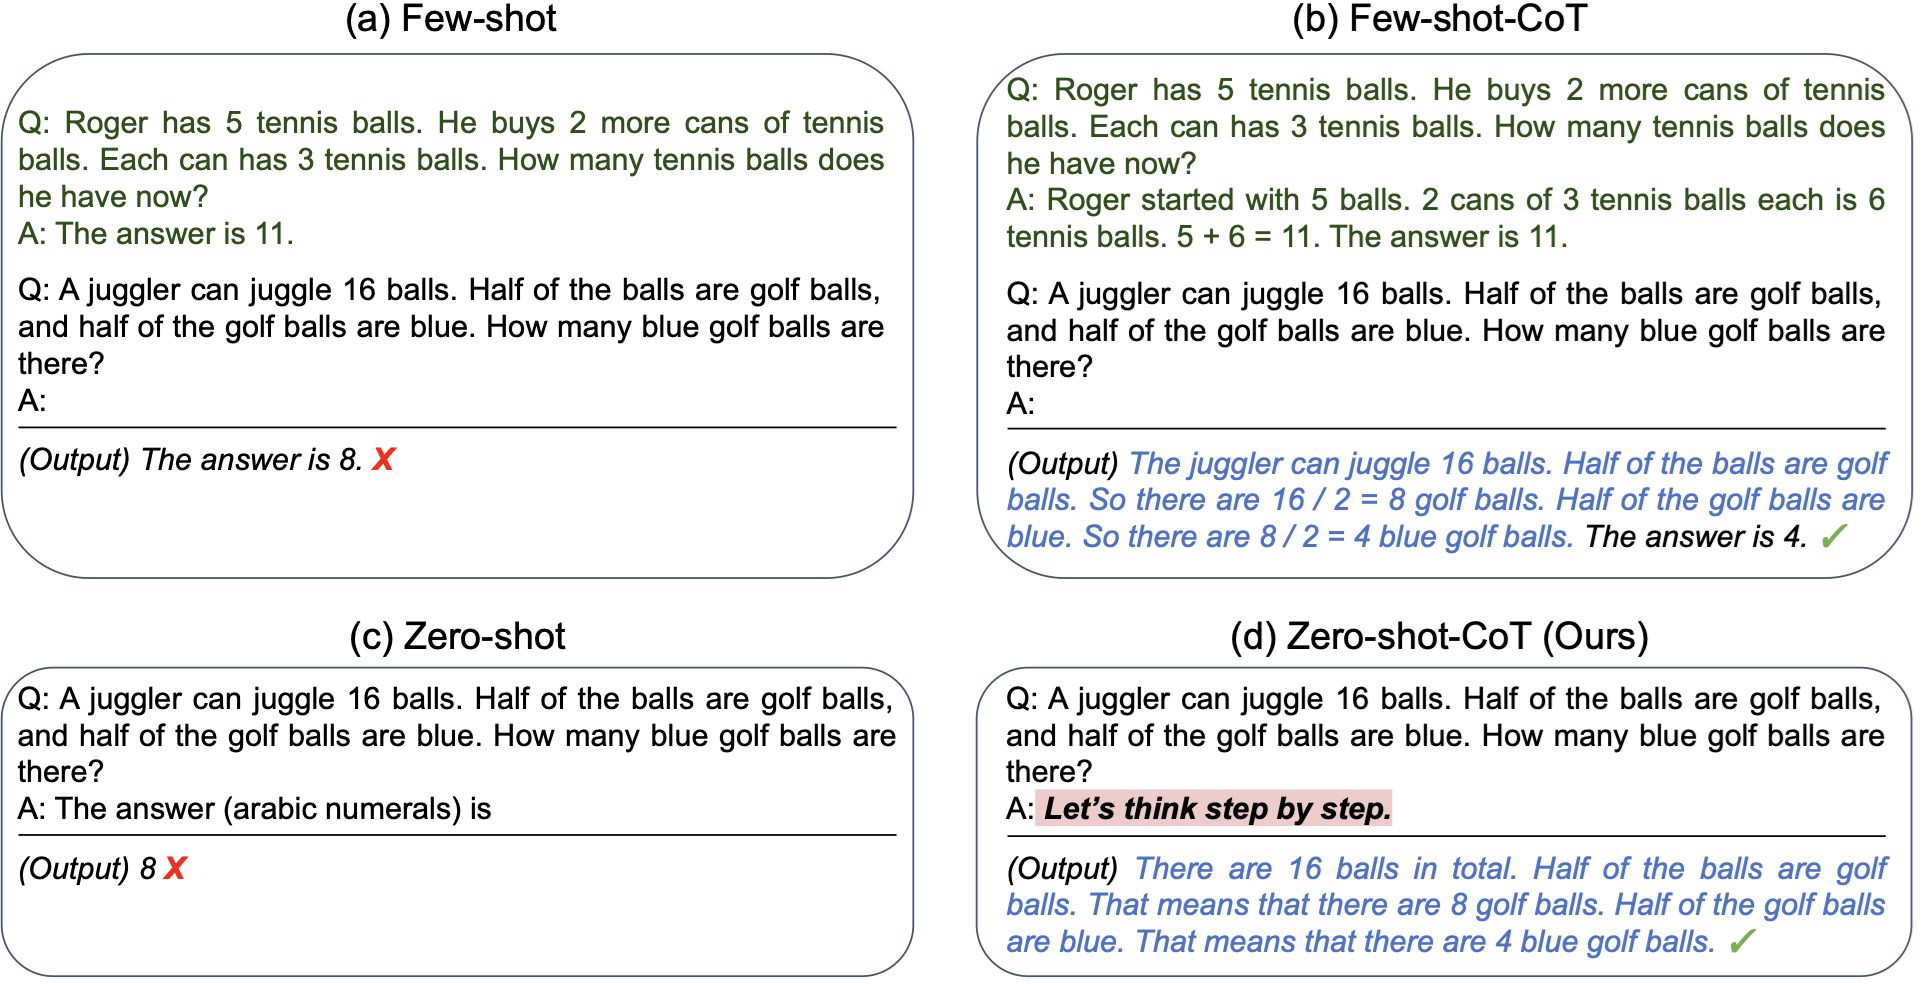
\includegraphics[width=0.9\textwidth]{./Figures/prompting.png}
	\caption{Ejemplo de uso de técnicas de \textit{prompting}.}
	\label{fig:prompting}
\end{figure}

A su vez, la ingeniería de \textit{prompts} ha demostrado ser fundamental en aquellos contextos en los que
el \textit{fine-tuning} no es viable, ya que hay muchos modelos cerrados que solo son accesibles a través de una API
y la capacidad de modificar su comportamiento sin reentrenamiento se vuelve crucial.
Por lo tanto, esta técnica se convierte en una herramienta práctica, eficiente y cada vez más sofisticada
para adaptar modelos generalistas a tareas específicas.

%----------------------------------------------------------------------------------------
%	SECTION 4
%----------------------------------------------------------------------------------------

\section{Ajuste fino}
El ajuste fino (\textit{fine-tuning}) \cite{howard2018universal} es una técnica de entrenamiento de modelos extensos de lenguaje 
que permite adaptar un modelo previamente entrenado a una tarea en específico.
A diferencia del entrenamiento desde cero, esta técnica parte de una base
y lo especializa utilizando un conjunto mucho más pequeño y específico de datos.
De este modo se reduce significativamente el coste computacional a la vez que se aprovecha
la capacidad predictiva del modelo del que se parte.

Para llevar a cabo el ajuste fino, se conservan la estructura y los parámetros previamente entrenados del modelo base,
evitando así la necesidad de un entrenamiento completo desde cero.
En la práctica, el proceso de \textit{fine-tuning} suele centrarse en modificar únicamente una parte reducida del modelo,
como las capas superiores, que son las más cercanas a la salida y, por tanto,
más fácilmente adaptables a tareas específicas.
Alternativamente, pueden integrarse nuevas capas que se entrenan sin alterar el resto del modelo.
Esta aproximación permite preservar los conocimientos generales adquiridos durante el preentrenamiento
mientras se optimiza la capacidad del modelo para tareas concretas.

Además, en escenarios con recursos computacionales limitados
se utilizan técnicas de ajuste fino eficiente (parameter-efficient fine-tuning, PEFT),
como LoRA (\textit{Low-Rank Adaptation}) \cite{hu2021lora},
\textit{prefix tuning} \cite{li2021prefix} o \textit{prompt tuning}.
Estas estrategias reducen la cantidad de parámetros que deben entrenarse,
lo que no solo disminuye el tiempo de ajuste y el consumo de memoria,
sino que también facilita la reutilización del modelo base en múltiples contextos sin interferencia entre tareas.

Al adaptar un modelo generalista a contextos específicos,
se logra una mejora sustancial en la precisión, relevancia y
sensibilidad del modelo frente a matices del lenguaje propios del área de aplicación.
No obstante, es fundamental contar con datos de alta calidad y
bien etiquetados para evitar la sobreespecialización o la introducción de sesgos.

\pagebreak
%----------------------------------------------------------------------------------------
%	SECTION 5
%----------------------------------------------------------------------------------------
\section{LM Studio y otras tecnologías}
LM Studio \cite{lmstudio} es una plataforma de código abierto diseñada para facilitar la interacción
y despliegue de modelos extensos de lenguaje (LLM) de manera local,
lo que permite a los usuarios ejecutar y experimentar con modelos sin depender de servicios en la nube.
Esta herramienta destaca por su integración sencilla, soporte para múltiples formatos de modelos y una interfaz amigable.

Una de las ventajas clave de LM Studio es su capacidad para manejar modelos grandes y complejos con eficiencia.
Ofrece funcionalidades como la gestión de memoria optimizada,
soporte para cuantización y carga progresiva de modelos
lo que permite que usuarios con recursos limitados puedan aprovechar la potencia de los LLM
sin necesidad de infraestructura costosa.
Además, LM Studio facilita la personalización de modelos mediante interfaces accesibles,
lo que la convierte en una opción popular tanto para investigadores como para desarrolladores
que desean incorporar inteligencia artificial avanzada en sus proyectos.

Para la implementación del \textit{backend} de la aplicación que interactúa con LM Studio, se utilizó \textit{Python},
un lenguaje de programación ampliamente adoptado en el ámbito de la inteligencia artificial por su simplicidad
y la gran cantidad de bibliotecas disponibles.
Se empleó la biblioteca de FastAPI \cite{fastapi} en al construcción del servidor web gracias a su sintaxis intuitiva,
lo que facilitó la creación de \textit{endpoints} eficientes para la comunicación entre el usuario y el modelo.

Por otro lado, \textit{PyTorch} \cite{pytorch} es la biblioteca de referencia para el desarrollo 
y entrenamiento de modelos de aprendizaje profundo, incluyendo los LLM.
Proporciona una interfaz dinámica y flexible que permite tanto el entrenamiento
como la inferencia eficiente en hardware acelerado, y es compatible con múltiples plataformas. 
	\chapter{Diseño e implementación} % Main chapter title
\label{Chapter3} % Change X to a consecutive number; for referencing this chapter elsewhere, use \ref{ChapterX}
En este capítulo se detalla cómo se ha ejecutado la implementación del trabajo,
incluyendo la arquitectura del sistema, procesamiento de peticiones,
modelos extensos de lenguaje utilizados y las técnicas empleadas sobre la inteligencia artificial.
Adicionalmente, se incluyen los hallazgos intermedios significativos que fueron fundamentales para la implementación final.

\definecolor{mygreen}{rgb}{0,0.6,0}
\definecolor{mygray}{rgb}{0.5,0.5,0.5}
\definecolor{mymauve}{rgb}{0.58,0,0.82}

%%%%%%%%%%%%%%%%%%%%%%%%%%%%%%%%%%%%%%%%%%%%%%%%%%%%%%%%%%%%%%%%%%%%%%%%%%%%%
% parámetros para configurar el formato del código en los entornos lstlisting
%%%%%%%%%%%%%%%%%%%%%%%%%%%%%%%%%%%%%%%%%%%%%%%%%%%%%%%%%%%%%%%%%%%%%%%%%%%%%
\lstset{ %
  backgroundcolor=\color{white},   % choose the background color; you must add \usepackage{color} or \usepackage{xcolor}
  basicstyle=\footnotesize,        % the size of the fonts that are used for the code
  breakatwhitespace=false,         % sets if automatic breaks should only happen at whitespace
  breaklines=true,                 % sets automatic line breaking
  captionpos=b,                    % sets the caption-position to bottom
  commentstyle=\color{mygreen},    % comment style
  deletekeywords={...},            % if you want to delete keywords from the given language
  %escapeinside={\%*}{*)},          % if you want to add LaTeX within your code
  %extendedchars=true,              % lets you use non-ASCII characters; for 8-bits encodings only, does not work with UTF-8
  %frame=single,	                % adds a frame around the code
  keepspaces=true,                 % keeps spaces in text, useful for keeping indentation of code (possibly needs columns=flexible)
  keywordstyle=\color{blue},       % keyword style
  language=[ANSI]C,                % the language of the code
  %otherkeywords={*,...},           % if you want to add more keywords to the set
  numbers=left,                    % where to put the line-numbers; possible values are (none, left, right)
  numbersep=5pt,                   % how far the line-numbers are from the code
  numberstyle=\tiny\color{mygray}, % the style that is used for the line-numbers
  rulecolor=\color{black},         % if not set, the frame-color may be changed on line-breaks within not-black text (e.g. comments (green here))
  showspaces=false,                % show spaces everywhere adding particular underscores; it overrides 'showstringspaces'
  showstringspaces=false,          % underline spaces within strings only
  showtabs=false,                  % show tabs within strings adding particular underscores
  stepnumber=1,                    % the step between two line-numbers. If it's 1, each line will be numbered
  stringstyle=\color{mymauve},     % string literal style
  tabsize=2,	                   % sets default tabsize to 2 spaces
  title=\lstname,                  % show the filename of files included with \lstinputlisting; also try caption instead of title
  morecomment=[s]{/*}{*/}
}


%----------------------------------------------------------------------------------------
%	SECTION 1
%----------------------------------------------------------------------------------------
\section{Arquitectura del sistema}

Los primeros esfuerzos en el desarrollo del trabajo se enfocaron en definir el conjunto de módulos que compondrían la solución.
Estos componentes fueron identificados correctamente desde el principio:
un servidor \textit{web} y un módulo de modelos extensos de lenguaje.
Sin embargo, su relación en el sistema sí cambió durante la fase de implementación.

Inicialmente, durante la fase de diseño, se concibió que el servidor \textit{web} también alojaría el modelo extenso de lenguaje 
y sería responsable de gestionar su conjunto de datos, entrenamiento y despliegue.
Esta decisión se tomó al principio de la implementación,
influenciada por la forma en la que se trabaja con redes neuronales sencillas.
Hacer que esa arquitectura funcionase en este trabajo era mucho más complejo de lo estimado
por la propia naturaleza de los modelos extensos de lenguaje.
La incertidumbre generada por la ausencia de un conjunto de datos de calidad y tamaño suficientes,
y la dificultad implícita de reentrenar un modelo tan grande,
fueron un factor de riesgo permanente durante la fase de diseño.

Fue necesario profundizar en las materias de procesamiento de lenguaje natural y \textit{Large Language Models} \cite{fiubaLlm}
para definir una solución efectiva a este problema.
Finalmente se decidió por no solo ``extraer'' el módulo de modelos extensos de lenguaje del servidor \textit{web}
sino por simplificar su complejidad de programación haciendo uso de la herramienta LM Studio.
Este programa permite administrar los modelos locales de la computadora,
añadir nuevos a través de una interfaz de descarga
y hacer uso del hardware disponible para arrancarlos de forma transparente para el usuario.
Además, cuenta con varias ventanas de configuración de parámetros de lanzamiento del modelo, \textit{prompts} personalizados,
salida estructurada a través de un esquema JSON,
opciones relacionadas con la aleatoriedad y temperatura de la inferencia y otras características experimentales.

De este modo, el servidor \textit{web} también se simplificó en el desarrollo, ahorró mucho trabajo de programación sin
comprometer la calidad del proceso de la inteligencia artificial.
Esto también es coherente con la arquitectura de servidor ligero esperable en un prototipo
y tiene una mejor sinergia con bibliotecas orientadas al despliegue de servidores sencillos.

Tal y como se muestra en la figura \ref{fig:sist},
el prototipo es accesible para los clientes a través del protocolo HTTP-REST que expone el servidor.
Además, durante el desarrollo se implementó una sencilla página \text{web} para realizar peticiones de prueba
y mostrar la salida de texto obtenida.

\begin{figure}[htbp]
	\centering
	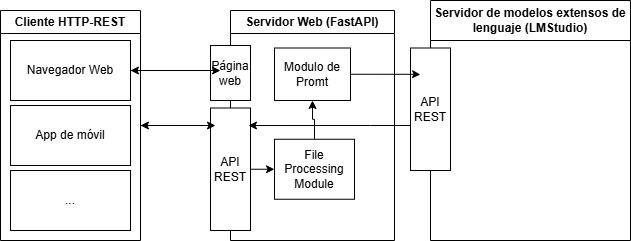
\includegraphics[width=0.9\textwidth]{./Figures/Sistema_es.png}
	\caption{Arquitectura del sistema.}
	\label{fig:sist}
\end{figure}

Otra ventaja de haber diseñado ambos módulos de forma independiente es que facilita al cliente
profundizar de forma paralela en los componentes sin comprometer el funcionamiento del resto del sistema.
Puede decidir si sustituir la implementación de uno u ambos módulos, escalarlos y distribuirlos en distintos entornos
para ajustarlo a su aplicación para \text{smartphones} y plan de expansión de servicios. 

%----------------------------------------------------------------------------------------
%	SECTION 2
%----------------------------------------------------------------------------------------
\section{Procesamiento de peticiones \textit{web} y ficheros}
Para la implementación del servidor web se decidió utilizar la biblioteca de FastAPI \cite{fastapi}.
Es una biblioteca moderna y de alto rendimiento para la construcción de APIs \text{web} en Python,
diseñada sobre estándares como OpenAPI \cite{openapi} y JSON schema.
Ofrece una forma rápida y eficiente de desarrollar interfaces REST
con una sintaxis sencilla y basada en anotaciones.
Esto permite una validación automática de datos de entrada y generación de documentación.
Todo esto hace que FastAPI sea una opción ideal para construir microservicios y prototipos rápidos.

El servidor expone dos servicios principales.
El primero es un \textit{endpoint} de tipo GET que proporciona la página \textit{web} que visualiza la interfaz gráfica del prototipo.
El otro servicio implementa un método POST para recibir las peticiones de consulta por parte del usuario para su procesamiento
y reenvío al módulo de inteligencia artificial. 


\pagebreak
\subsection{Procesamiento de peticiones}
En la figura \ref{fig:flux} se representa el diagrama de flujo correspondiente al manejo de las peticiones entrantes.

\begin{figure}[htbp]
	\centering
	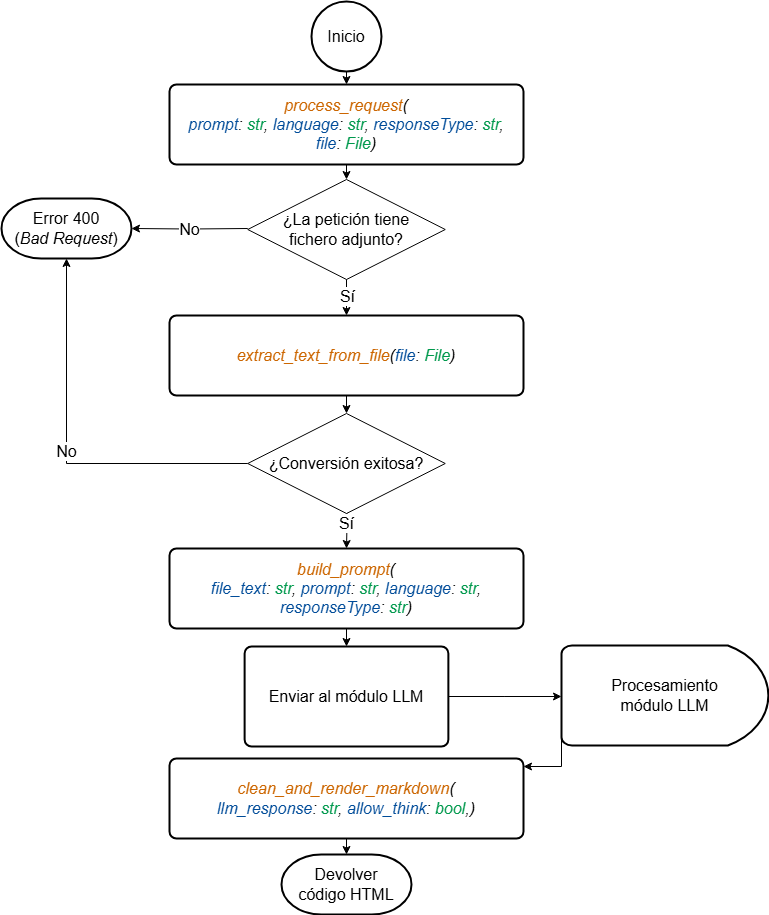
\includegraphics[width=1\textwidth]{./Figures/flux-diagram.png}
	\caption{Diagrama de flujo del procesamiento de peticiones.}
	\label{fig:flux}
\end{figure}

El proceso comienza cuando el cliente envía una solicitud con los datos de consulta a través de un cliente REST.
Esto puede ser a través del formulario proporcionado por el servidor o a través de cualquier otra herramienta como,
por ejemplo, PostMan.
Tras realizar las comprobaciones iniciales,
el servidor continúa procesando la información mediante una serie de funciones específicas:
\begin{itemize}
\item \texttt{extract\_text\_from\_file}:
es el proceso encargado de extraer la información textual de los ficheros adjunto
y formatearlo para que el módulo de modelos extensos de lenguaje sea capaz de interpretarlo.
En esta función se hace uso de las bibliotecas de cgardet, docx y fitz para la detección del formato y
su conversión a texto plano.
\item \texttt{build\_prompt}:
esta función es la encargada de construir el \textit{prompt} a partir del texto extraído del fichero
y las entradas adicionales proporcionadas por el usuario, entre las que se incluyen el idioma de
la respuesta, el tipo de listado que se solicita y algunas instrucciones adicionales.
En esta función se emplea la ingeniería de \textit{prompting} que se envía posteriormente al módulo LLM.
Se detalla más adelante en la sección \ref{subsec:prompt}.
\item \texttt{clean\_and\_render\_markdown}:
esta función se encarga de limpiar la salida y formatearla en código HTML
a través de la biblioteca markdown para una mejor legibilidad en navegadores web.
\end{itemize}

Cabe destacar que para la comunicación con el módulo LLM,
aunque LM Studio ofrece un SDK en Python para interactuar mediante programación,
se optó por utilizar su interfaz REST.
La razón es que así el servidor \textit{web} no depende exclusivamente de la biblioteca de LM Studio.
Al emplear un protocolo de comunicación estándar como REST,
el servidor web puede interactuar fácilmente con cualquier otro servicio que aloje modelos extensos de lenguaje,
lo que le da mayor flexibilidad.

\subsection{Interfaz gráfica}
El servidor también facilita el acceso a una página \textit{web} con la interfaz gráfica del prototipo,
tal y como se aprecia en la figura \ref{fig:webPage}.

\begin{figure}[htbp]
	\centering
	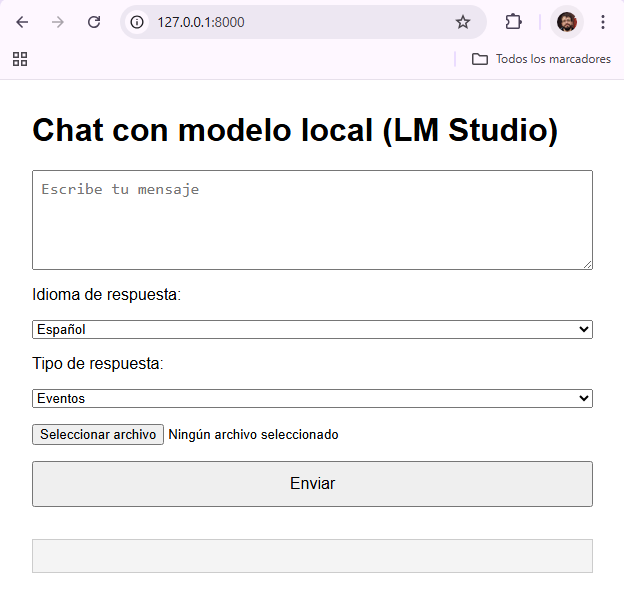
\includegraphics[width=0.8\textwidth]{./Figures/webpage.png}
	\caption{Interfaz gráfica del prototipo.}
	\label{fig:webPage}
\end{figure}

El formulario consta de los siguientes elementos:
\begin{itemize}
\item Cuadro de texto:
este elemento se utiliza para darle las instrucciones específicas a la inteligencia artificial.
Está pensado para que sea un mensaje breve y conciso que pueda ayudar al usuario a guiar un poco mejor la respuesta.
Es un parámetro opcional y puede dejarse en blanco.
\item Idioma de respuesta:
se trata de un \textit{combobox} que contiene dos opciones: inglés y español.
El módulo LLM responderá en el idioma seleccionado, independientemente del idioma del fichero de entrada.
Este elemento se añadió porque algunos modelos presentan comportamientos anómalos si responden en un idioma distinto al inglés.
\item Tipo de respuesta:
permite a la inteligencia artificial centrar su respuesta en un aspecto concreto de la narrativa.
Al estar instruida en devolver listas de elementos, la idea es que el usuario pueda elegir la opción
específica de la creación de mundos que le interese.
\item Fichero adjunto:
es el elemento más importante del formulario.
El usuario puede agregar un fichero con el contexto narrativo existente
y enviarlo a la inteligencia artificial para que genere nuevo contenido.
\end{itemize}

%----------------------------------------------------------------------------------------
%	SECTION 3
%----------------------------------------------------------------------------------------
\section{Gestión de modelos extensos de lenguaje}
El siguiente paso en la fase de implementación fue la instalación
y configuración del módulo de modelos extensos de lenguaje.
Inicialmente, se analizó si la gestión y comunicación con la LLM se haría a través de una
API en la nube o alojarlo localmente en el servidor \textit{web}.

La opción de la API implicaba depender de servicios externos
en internet, lo que resultaba en peores tiempos de respuesta y un coste adicional significativo
debido a los modelos de pago por uso que restringen la cantidad de consultas.
A su vez, la interacción con servicios externos exponía la información transmitida en las consultas
lo que podría incumplir los requerimientos de protección de la privacidad
y propiedad intelectual de los datos del cliente.
También se observó un menor número de modelos disponibles y opciones de personalización,
lo que dificultaba la experimentación y adaptación de los LLM a las necesidades específicas del sistema.

Por otra parte, la opción de gestionar los modelos extensos de lenguaje
de forma nativa presentaba desafíos considerables.
Desarrollar la infraestructura \textit{software} necesaria para la gestión de modelos
era una tarea con alta complejidad técnica que iba más allá de la mera integración de \textit{frameworks}.
Esto podía suponer limitaciones significativas en el proceso de configuración de los modelos y,
en consecuencia, provocar un coste elevado en términos de tiempo y recursos de desarrollo.

Por estos motivos se decidió buscar alternativas para este módulo y se encontraron varias herramientas que
cumplían con las características deseadas, y las más llamativas fueron
Ollama \cite{ollama}, GPT4All \cite{gpt4all} y LM Studio \cite{lmstudio}.
Esta última fue la opción elegida eventualmente por su interfaz intuitiva y buscador de modelos,
además de simplificar la gestión y configuración de los LLM.
Alojar localmente los modelos permite el envío ilimitado de consultas
y cumple con los requisitos de privacidad de los datos del cliente.

En los siguientes apartados se detallan los distintos procesos de gestión que se llevaron a cabo con LM Studio.

\subsection{Descarga de modelos}
El menú \textit{discover} de LM Studio da acceso al explorador de modelos extensos de lenguaje,
permitiendo a los usuarios navegar por una vasta biblioteca alojada principalmente en la plataforma Hugging Face \cite{huggingface}.
Como se ilustra en la figura \ref{fig:downloadMenu},
esta herramienta de búsqueda facilita la localización de modelos específicos mediante filtros por nombre o palabras clave,
presentando los resultados en un listado que se ajusta a los criterios definidos.
Al seleccionar un modelo, se muestra una sección de detalles con sus características y las distintas opciones de descarga disponibles.

\begin{figure}[htbp]
	\centering
	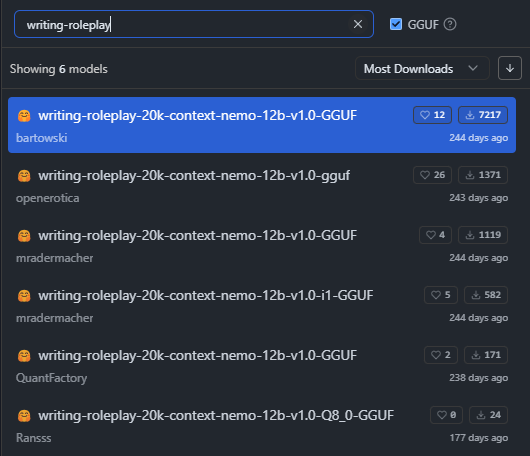
\includegraphics[width=0.8 \textwidth]{./Figures/download_menu.png}
	\caption{Buscador de modelos de LM Studio.}
	\label{fig:downloadMenu}
\end{figure}

Esta herramienta se empleó para la búsqueda y descarga de múltiples modelos,
que se enumeran y detallan en la subsección \ref{subsec:modelos-llm}.
Se eligieron tanto modelos generalistas como aquellos especializados en \textit{roleplay},
con el fin de analizar y comparar su rendimiento en tareas de construcción de mundos.

\subsection{Administración y configuración de modelos}
LM Studio permite la gestión y configuración de los modelos locales en el menú \textit{My Models}.
Además de listar los LLM descargados en el equipo, esta ventana permite personalizar
sus parámetros de ejecución para optimizar el rendimiento y la precisión de las respuestas.

\pagebreak
Como se muestra en la figura \ref{fig:configMenu},
al seleccionar un modelo se tiene acceso a un conjunto de ajustes agrupados
en varios conjuntos.
Como se trabajó en el \textit{prompting} en el servidor \textit{web},
los esfuerzos de configuración se centraron en los parámetros de carga e inferencia.

\begin{figure}[htbp]
	\centering
	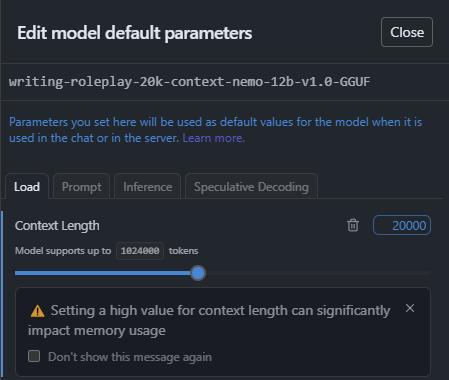
\includegraphics[width=0.8 \textwidth]{./Figures/config_menu.png}
	\caption{Configurador de modelos de LM Studio.}
	\label{fig:configMenu}
\end{figure}

La longitud del contexto resultó ser un parámetro fundamental en el trabajo.
Dado que las consultas de los usuarios se espera que vengan acompañadas de relatos extensos de \textit{worldbuilding},
era crucial que el LLM pudiera procesar y comprender grandes volúmenes de texto para generar respuestas coherentes y relevantes.
Los modelos tienen configurado por defecto un tamaño de contexto de 2048 o 4096 \textit{tokens},
un valor muy por debajo del tamaño de petición que se estima.

Para superar esta limitación, se seleccionó un tamaño de contexto compatible con las capacidades relativas de cada modelo,
a menudo indicado en los detalles.
Esta configuración fue esencial para asegurar que los LLM pudieran asimilar la totalidad de los relatos proporcionados.
Adicionalmente, se exploraron diversas tácticas para gestionar el exceso de contexto,
resultando más eficaces el acortamiento desde el principio de la secuencia o desde su punto medio.

Los parámetros de configuración de inferencia más importantes fueron la temperatura y
las técnicas de muestreo de probabilidad, como Top P o Top K.
Durante el desarrollo del proyecto, se observó que los valores predeterminados para estas variables
ya eran bastante adecuados. Por eso, solo fue necesario hacer ajustes mínimos en algunas de ellas.

Por defecto todos los modelos incluyen una sección de razonamiento.
Este parámetro fue deshabilitado en la configuración del modelo
y se filtró en el post-procesamiento para que no se mostrara en la respuesta al usuario.

\pagebreak
\subsection{Ejecución de modelos e interfaz REST}
La herramienta muestra y administra qué LLMs están activos y cargados en la memoria del sistema.
Además, también puede desplegar con un solo \textit{click} un servidor local compatible con la interfaz REST de OpenAI.
Cuando las peticiones llegan a este servidor, se registran en un log detallado que no solo proporciona
información sobre su estado sino que también muestra datos cruciales para la depuración de salidas incorrectas o errores.

\begin{figure}[htbp]
	\centering
	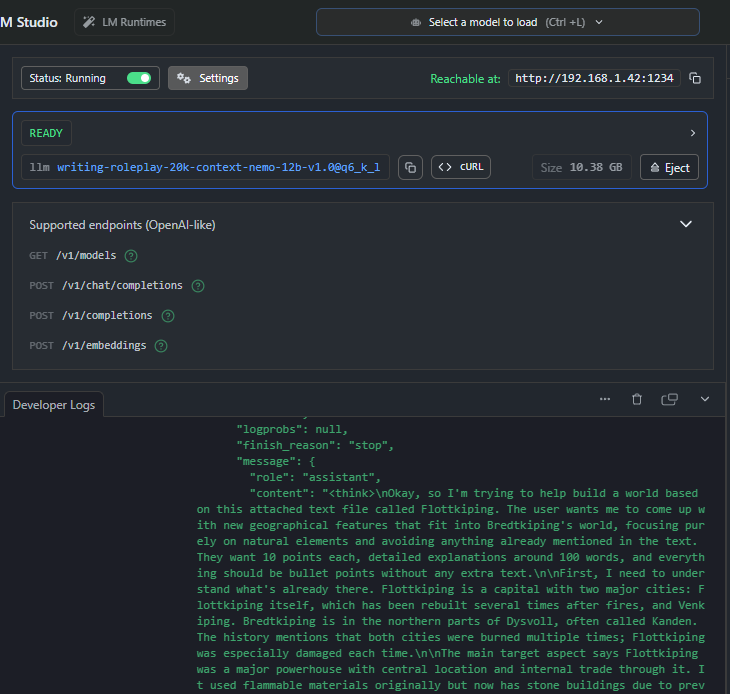
\includegraphics[width=1.0 \textwidth]{./Figures/developer_menu.png}
	\caption{Menú de desarrollador de LM Studio.}
	\label{fig:developerMenu}
\end{figure}

Una vez el modelo y el servidor están activos, el flujo del procesamiento de peticiones de la solución está completo.
El LLM, ya configurado con el tamaño de contexto ampliado y los parámetros de aleatoriedad ajustados,
gestiona la entrada, generando las respuestas esperadas.
Este diseño permite la misma forma de gestionar las peticiones,
sin importar el modelo que esté activo.

\pagebreak
\subsection{Modelos extensos de lenguaje utilizados}\label{subsec:modelos-llm}
El conjunto de modelos empleados en este trabajo se obtuvo a través de la herramienta de descarga de LM Studio.
Fueron seleccionados con un número de parámetros y un nivel de cuantización adecuado,
sin superar el límite de 12~GB de tamaño en memoria RAM dedicada en la tarjeta gráfica.
Esta parametrización permite aprovechar al máximo las capacidades del \textit{hardware} disponible,
con el objetivo de evaluar el rendimiento de distintos LLMs en tareas de generación narrativa.
En la tabla~\ref{tab:modelos_llm} se detallan las características de cada modelo:

\begin{table}[h]
\centering
\caption{Modelos extensos de lenguaje utilizados en el trabajo.}
\resizebox{\textwidth}{!}{%
\begin{tabular}{l l c c c r}
\toprule
\textbf{Modelo} & \textbf{Editor} & \textbf{Arquitectura} & \textbf{Parámetros} & \textbf{Cuantización} & \textbf{Tamaño (Contexto / VRAM)} \\
\midrule
\texttt{arliai-rpmax-v1.4} & bartowski & Mistral & 24 B & Q3\_K\_S & 20 k tokens / 10,40 GB \\
\texttt{writing-roleplay-v1.0} & bartowski & LLaMA & 12 B & Q6\_K\_L & 20 k tokens / 10,38 GB \\
\texttt{worldbuilder} & mrademacher & LLaMA & 12 B & Q6\_K & 4k tokens / 10,06 GB \\
\texttt{deepseek-r1-distill} & lmstudio & Qwen2 & 7 B & Q4\_K\_M & 32 k tokens / 4,68 GB \\
\texttt{mistral-instruct-v0.1} & TheBloke & Mistral & 8 B & Q8\_0 & 20 k tokens /  7,70 GB \\
\bottomrule
\end{tabular}%
}
\label{tab:modelos_llm}
\end{table}

Los tres primeros modelos referenciados fueron refinados específicamente para tareas de \textit{roleplay} y \textit{worldbuilding}.
Esto permite una mejor comprensión del fichero proporcionado por el usuario y una generación de contenido narrativo más coherente y contextualizado.

Con el fin de evaluar el rendimiento del sistema con las alternativas ampliamente accesibles en línea,
se incorporaron dos modelos generalistas que actúan como referencia.
Dado que estos modelos no han sido entrenados explícitamente para la creación narrativa,
la estrategia permite evaluar tanto la eficacia de la ingeniería de \textit{prompting} implementada,
como el impacto del entrenamiento específico en la capacidad de análisis del contexto y la calidad de las respuestas generadas.

%----------------------------------------------------------------------------------------
%	SECTION 4
%----------------------------------------------------------------------------------------
\section{Personalización del \textit{prompt} en función del servicio}

Una de las funcionalidades clave del sistema implementado consiste en la generación de la instrucción
a partir de la información proporcionada por el usuario en la petición.
Para guiar de forma efectiva la salida del modelo y obtener respuestas que cumplieran con los requerimientos del cliente,
se recurrió a diversas técnicas de ingeniería de \textit{prompting}.

\subsection{Función generadora de la instrucción}
\label{subsec:prompt}
Para aterrizar la lógica requerida se desarrolló en el módulo de \textit{prompt} la función \textit{build\_prompt}
y cuyo código se muestra debajo de este párrafo.
Este método se encarga de construir la instrucción alrededor del contexto narrativo,
extraído previamente del texto del fichero adjunto,
y combinarlo de forma estructurada con el resto de elementos de entrada.

\pagebreak
\begin{lstlisting}[label=cod:prompt,caption=Estructura de la función que construye la instrucción para el modelo.]
def build_prompt(file_text, additional_instructions, language, response_type):
    if response_type not in prompts:
        raise ValueError(
            f"Invalid output_type: '{response_type}'. Must be one of {list(prompts.keys())}"
        )

    general_prompt = prompts["general"]
    specific_prompt = prompts[response_type]

    content = (
        f"{general_prompt}\n"
        f"=== ATTACHED TEXT FILE ===\n"
        f"{file_text}\n\n"
        f"=== ADDITIONAL INSTRUCTIONS ===\n"
        f"{additional_instructions}"
        f"======\n"
        f"{specific_prompt}\n\n"
        f"Answer only in {language}.\n\n"
    )

    return {"role": "user", "content": content}

\end{lstlisting}

A continuación, se definen los elementos principales en orden secuencial:
\begin{itemize}
\item \textit{response\_type}:
tipo de salida esperada por parte del modelo.
Este parámetro selecciona el \textit{prompt} específico dentro del conjunto de \textit{prompts},
y si el valor proporcionado no se encuentra definido en dicho conjunto, se lanza una excepción.
\item \textit{general\_prompt}:
fragmento introductorio de la instrucción, común para todos los tipos de respuesta, que establece el rol
y las directrices principales que tiene que seguir el modelo.
\item \textit{specific\_prompt}:
instrucción particular asociada al tipo de respuesta especificado en \texttt{response\_type}.
Complementa a la instrucción principal añadiendo detalles o restricciones más concretas,
adaptadas a la tarea específica que debe realizar el modelo.
\item \textit{file\_text}:
contenido del archivo de entrada con el contexto narrativo sobre el cual se construye
la instrucción que es enviada al modelo.
\item \textit{additional\_instructions}:
conjunto de instrucciones adicionales proporcionadas por el usuario.
Estas indicaciones permiten personalizar o enriquecer el comportamiento del modelo
y ajustar la respuesta a necesidades específicas.
\item \textit{language}:
idioma en el que debe responder el modelo.
Esta indicación se incluye al final del mensaje para garantizar que
la salida esté redactada exclusivamente en el idioma solicitado.
\end{itemize}

Esta implementación permite personalizar la instrucción de manera precisa según la categoría de respuesta
y otras variables contextuales.
Gracias a este enfoque basado en la técnica de \textit{prompt chaining},
se reduce significativamente la complejidad de la interacción entre el usuario y el modelo de lenguaje.
Además, garantiza una respuesta precisa sin necesidad de que el usuario, 
que previsiblemente utilizará el servicio desde un dispositivo con pantalla reducida,
posea conocimientos en ingeniería de \textit{prompting}.

\subsection{Refinado iterativo de las instrucciones}
Una vez se definió la estructura general del mensaje, el siguiente paso consistió en optimizar tanto la instrucción general
como las indicaciones específicas asociadas a cada elemento de la ambientación narrativa. 
Este proceso fue esencial para garantizar que las respuestas generadas por los modelos se alinearan con las
expectativas propias de un asistente creativo que proporcionara listas de nuevas ideas.

El refinamiento se llevó a cabo de forma iterativa, como se muestra en la figura \ref{fig:iterativeRefinement},
a través de prueba y error con múltiples variantes para las instrucciones.
En cada ciclo se evaluaron las respuestas del modelo en función tanto de la estructura del contenido como de su coherencia
con el contexto narrativo aportado.
Esto permitió identificar errores en la formulación del \textit{prompt} responsables de alucinaciones,
repeticiones de información y otras inconsistencias en la generación de texto de los modelos.
En función del reto encontrado, se analizó la forma de solucionarlo mediante el empleo de técnicas
entre las que se encuentran \textit{chain of thought}, \textit{instruction-based prompting},
\textit{constrained-output prompting} y \textit{negative prompting}.

\begin{figure}[htbp]
	\centering
	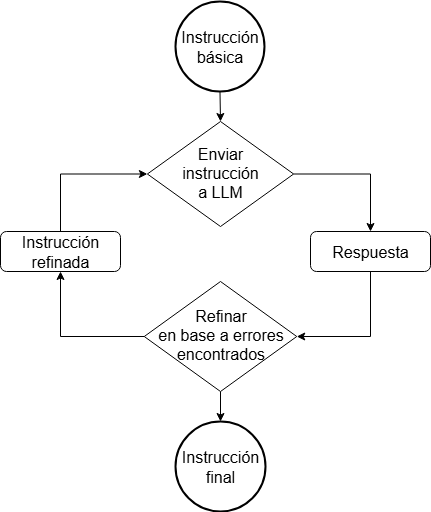
\includegraphics[width=0.7 \textwidth]{./Figures/iterative-process.png}
	\caption{Proceso de refinamiento de instrucciones.}
	\label{fig:iterativeRefinement}
\end{figure}

\pagebreak
En estre proceso se trabajó sobre cinco instrucciones diferentes:
\begin{itemize}
\item General:
se centró en resolver los problemas comunes detectados en todas las categorías narrativas.
En versiones iniciales, el modelo no generaba listas de forma adecuada ni mantenía un formato consistente en la respuesta.
También mostró dificultades para distinguir entre el contexto narrativo y las instrucciones que debía seguir.
Esto derivaba en repeticiones de información ya presentes en el texto de referencia, lo que limitaba considerablemente
la originalidad y riqueza de sus propuestas.
Por estas razones, fue necesario reformular la instrucción 
mediante la incorporación de directrices explícitas sobre el objetivo del modelo,
el formato de salida y la distinción entre contexto e instrucciones.
Se establecieron requisitos claros sobre la longitud mínima de las listas,
el nivel de detalle esperado en cada punto
y la obligatoriedad de que todos los elementos fueran completamente nuevos.
\item Eventos:
se enfocó en guiar al modelo
hacia la generación de sucesos nuevos que enriquecieran el desarrollo del mundo narrativo
sin duplicar hechos ya mencionados en el texto base.
En versiones preliminares, el modelo tendía a reformular eventos existentes en lugar de inventar situaciones originales.
Esto es debido al fuerte entrenamiento de los modelos a no modificar hechos que se consideran históricos.
Para resolver esto, se eliminó la palabra ``histórico'' de la instrucción y
se reforzó la indicación de que los eventos debían ser completamente inéditos
y conectados de forma coherente con el contexto.
\item Personajes:
las versiones iniciales del \textit{prompt} no ofrecían suficientes indicaciones estructurales,
lo que resultaba en respuestas incompletas o poco claras.
Algunos personajes carecían de nombre, contexto o motivación dentro del mundo ficticio.
Para solventar esto, la instrucción fue reescrita para exigir explícitamente un nombre, apellido,
alias (si procede) y una explicación clara de la relación del personaje con la historia o el entorno.
\item Geografía:
fue afinada para evitar confusiones entre elementos naturales y construcciones humanas.
En iteraciones anteriores, el modelo a menudo mezclaba ríos o montañas con ciudades o estructuras artificiales,
y no siempre justificaba la relevancia geográfica de los elementos descritos.
Para corregir esto, se incorporó una aclaración sobre el tipo de elementos geográficos aceptados
y se exigió una descripción detallada de cada punto, así como su importancia ecológica,
simbólica o estratégica dentro del mundo narrativo.
\item Localizaciones:
buscó mejorar la claridad y especificidad de los núcleos poblacionales propuestos.
En las versiones previas, el modelo a menudo confundía localizaciones con elementos geográficos
o entregaba descripciones genéricas sin conexión con el resto del mundo,
al utilizar la palabra ``asentamientos'' hubo una mejoría notable en el rendimiento.
La nueva versión de la instrucción estableció que debían generarse únicamente poblaciones (ciudades, pueblos, países)
y que cada una debía incluir una descripción detallada de sus características culturales, políticas o históricas,
así como su función o importancia dentro del contexto narrativo.
\end{itemize}

\pagebreak
En este proceso se utilizaron diversos corpus como contexto
con el objetivo de contrastar el comportamiento de los modelos en distintas situaciones.
A modo de anécdota, uno de los textos empleados estaba ambientado en una franquicia conocida
y los LLM generaron respuestas que incluían información propia de ese universo,
a pesar de no estar explícitamente presente en el texto proporcionado.
Esto sugiere que fueron entrenados previamente con contenidos relacionados con dicha ambientación.

Se puede consultar la versión final de las instrucciones desarrolladas en este trabajo en el Anexo (FALTA REFERENCIA).
Dado que el inglés es el idioma preferente de los modelos,
las instrucciones se redactaron en ese idioma.
Por esto mismo, se incluye una instrucción final para que la respuesta se genere en el idioma seleccionado por el usuario.
Sin embargo, es importante señalar que no todos los modelos soportan el español,
lo que ocasionalmente lleva a que esta última instrucción sea ignorada.
Este fenómeno se detallará en la siguiente sección.
	% Chapter Template

\chapter{Ensayos y resultados} % Main chapter title

\label{Chapter4} % Change X to a consecutive number; for referencing this chapter elsewhere, use \ref{ChapterX}
En este capítulo se describe el conjunto de ensayos realizados sobre el sistema y se recopilan sus resultados.
Con este propósito, se explican las características del \textit{hardware} y el banco de pruebas que se emplearon.
Además, se explican los criterios de evaluación para determinar la calidad de las respuestas de los
modelos extensos de lenguaje.
Finalmente, se hace un análisis global de los resultados, destacando el grado de mejora que ofrece el sistema, así como
sus errores más comunes.

%----------------------------------------------------------------------------------------
%	SECTION 1
%----------------------------------------------------------------------------------------

\section{Entorno y banco de pruebas}
Los ensayos fueron ejecutados en un equipo de altas prestaciones, orientado a tareas de cómputo intensivo y procesamiento de modelos de lenguaje de gran tamaño.
Sus especificaciones son las siguientes:
\begin{itemize}
\item Memoria RAM: 64 GB.
\item Tarjeta gráfica: NVIDIA GeForce RTX4080 SUPER, con 16 GB de memoria RAM dedicada.
\item Procesador: AMD Ryzen9 7950X3D 16-Core.
\item Sistema Operativo: Windows 11.
\end{itemize}

Aunque se emplearon diversos \textit{worldbuildings} en el proceso iterativo de refinamiento de las instrucciones,
el contexto narrativo de prueba se basó exclusivamente en textos pertenecientes al mundo de ficción ``Aanrah'',
desarrollado por el autor Necrowmancer en la plataforma de WorldAnvil \cite{aanrah2024}.
Esta ambientación fue seleccionada por ofrecer una combinación equilibrada de complejidad conceptual,
léxico específico y coherencia interna, sin alcanzar un volumen excesivo de contenido.
Dicha elección refleja el tipo de entradas que previsiblemente introducirán los usuarios del sistema,
al tiempo que plantea un desafío suficientemente realista para los modelos extensos de lenguaje.
El corpus de referencia se encuentra detallado en el apéndice \ref{AppendixB}.

%----------------------------------------------------------------------------------------
%	SECTION 2
%----------------------------------------------------------------------------------------

\section{Pruebas de procesamiento de ficheros}
Para comprobar el funcionamiento del procesamiento de los ficheros sin depender del módulo de procesamiento de peticiones \textit{web},
se implementaron varias celdas en un \textit{notebook} de Jupyter.
Esta solución no solo permite evaluar de forma controlada el comportamiento del módulo,
sino que además cumple con los criterios de pruebas automatizadas exigidos por el cliente.

Además, se formateó el contexto narrativo de prueba en los tres tipos de fichero aceptados: txt, docx y pdf.
El funcionamiento del módulo quedó validado tras comprobar que el texto extraído de todos los ficheros es idéntico,
tal y como se muestra en las figuras \ref{fig:txt-read-test}, \ref{fig:docx-read-test} y \ref{fig:pdf-read-test}.
Se aprecian diferencias de formato en el archivo pdf, pero su contenido coincide.

\begin{figure}[htbp]
	\centering
	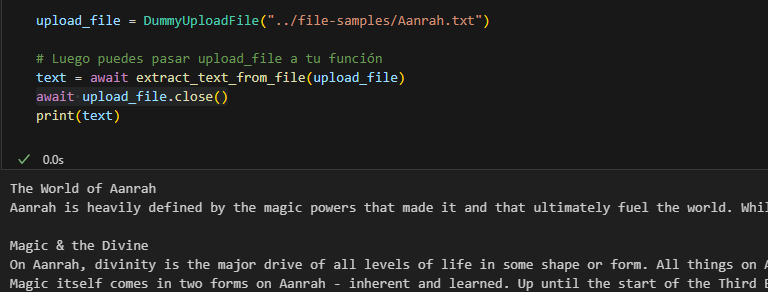
\includegraphics[width=0.9\textwidth]{./Figures/file-read-test-txt.png}
	\caption{Prueba de lectura de ficheros txt.}
	\label{fig:txt-read-test}
\end{figure}

\begin{figure}[htbp]
	\centering
	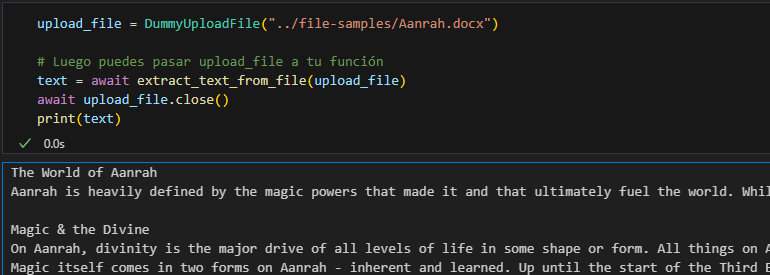
\includegraphics[width=0.9\textwidth]{./Figures/file-read-test-docx.png}
	\caption{Prueba de lectura de ficheros docx.}
	\label{fig:docx-read-test}
\end{figure}

\begin{figure}[htbp]
	\centering
	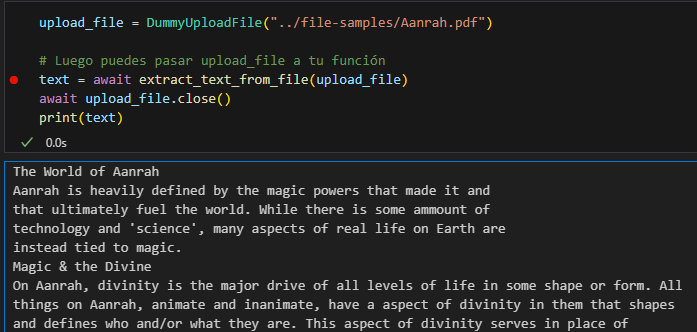
\includegraphics[width=0.9\textwidth]{./Figures/file-read-test-pdf.png}
	\caption{Prueba de lectura de ficheros pdf.}
	\label{fig:pdf-read-test}
\end{figure}

%----------------------------------------------------------------------------------------
%	SECTION 3
%----------------------------------------------------------------------------------------
\pagebreak
\section{Pruebas de procesamiento de peticiones web}
Durante la fase de implementación se llevaron a cabo pruebas incrementales que incluyeron
la verificación de la correcta carga del HTML, la recepción de las peticiones junto con los archivos adjuntos,
la lectura del contenido y, finalmente,
la integración completa del flujo de comunicación entre el usuario y el modelo extenso de lenguaje.
Cuando una petición se procesa correctamente, la información se envía de vuelta a la interfaz \textit{web},
donde se muestra en un cuadro de texto.

En la figura~\ref{fig:web-test} se muestra el resultado de una petición en la que,
con fines de prueba, se omitió el envío al módulo LLM
y en su lugar se devolvió directamente al usuario el contenido del fichero adjunto.

\begin{figure}[htbp]
	\centering
	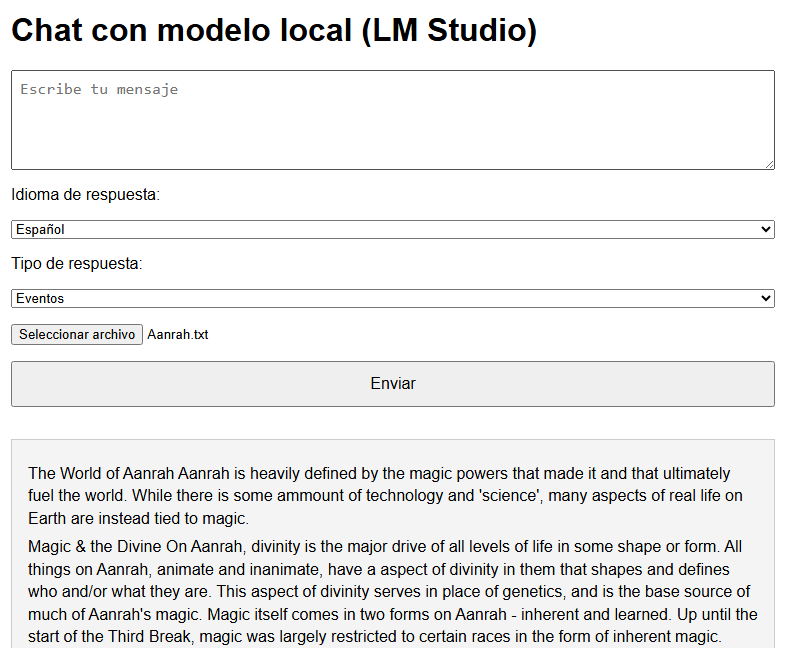
\includegraphics[width=1\textwidth]{./Figures/web-test.png}
	\caption{Prueba de envío de peticiones REST.}
	\label{fig:web-test}
\end{figure}

En las pruebas de los siguientes apartados se muestran múltiples figuras de la interfaz con el flujo completo de datos.

%----------------------------------------------------------------------------------------
%	SECTION 4
%----------------------------------------------------------------------------------------
\section{Método para valorar la salida de los modelos extensos de lenguaje}
En este apartado se explica la lógica que se siguió para valorar la calidad de las respuestas
generadas por el modelo de lenguaje.
Este proceso presenta una dificultad inherente:
debido a la naturaleza de los casos de uso del sistema, esta puntuación es completamente subjetiva.
Conceptos como “adecuación”, “originalidad” o “interés narrativo” no pueden medirse de forma objetiva ni automática,
lo que limita la posibilidad de una evaluación completamente reproducible.
Por ello, la validación fue realizada de forma manual, basándose en mi propio criterio como desarrollador del sistema.

Una vez aclarado este aspecto, las pruebas se estructuraron de forma que pudieran reproducirse de manera sencilla y sistemática.
En todas las evaluaciones se emplea el mismo fichero adjunto, que contiene el contexto narrativo base,
y se combina con cada tipo de elemento de \textit{worldbuilding} que se desea generar.
Este enfoque se aplica de forma consistente a todos los modelos extensos de lenguaje.
Adicionalmente, sobre este mismo conjunto de pruebas se compararán dos escenarios:
uno en el que se utiliza la ingeniería de \textit{prompting} desarrollada en este trabajo,
y otro en el que dicha técnica no se aplica.
Este contraste permitirá evaluar el impacto real de las instrucciones
refinadas sobre los modelos.

Para valorar la salida del modelo se emplearon los siguientes criterios:
\begin{itemize}
\item \textbf{Adecuación contextual}: se verifica que los elementos generados respeten el tono, estilo y detalles del contexto narrativo original.
\item \textbf{Pertinencia temática}: los resultados deben estar alineados con la categoría seleccionada
(por ejemplo, si se ha elegido ``personajes'', la salida no debe incluir ubicaciones o eventos).
\item \textbf{Originalidad}: se valora la capacidad del modelo para proponer ideas nuevas sin repetir explícitamente el contenido del fichero.
\item \textbf{Diversidad}: se analiza si la lista contiene variedad en las propuestas y evita repeticiones o elementos demasiado similares.
\item \textbf{Idioma}: se indica si el modelo acepta texto en español. 
\item \textbf{Consistencia}: analiza la inestabilidad en la respuesta de los modelos,
teniendo en cuenta que todos fueron configurados con una temperatura de 0,7 sobre 1. 
\item \textbf{Errores}: se listan los errores encontrados en las pruebas y se analiza el impacto que tienen.
\end{itemize}

%----------------------------------------------------------------------------------------
%	SECTION 5
%----------------------------------------------------------------------------------------
\section{Pruebas con modelos generalistas y \textit{prompting} poco preciso}
Esta sección analiza el rendimiento de los modelos que no han sido ajustados específicamente
para tareas de ambientación narrativa y que carecen de un refinamiento adecuado en las instrucciones.
El objetivo es simular los resultados que podrían obtenerse si una persona sin experiencia en ingeniería de
\textit{prompting} utilizara las opciones más comunes disponibles en línea.

Para lograr esto, se desactivó el módulo de \textit{prompts} y se bloquearon algunos controles de la interfaz
\textit{web} para que solo aceptara el fichero adjunto, el cuadro de texto y el selector de idiomas.
En la figura \ref{fig:prompt-test} se muestra
cómo el modelo responde libremente a la entrada del usuario.
Una vez validada la funcionalidad, todas las instrucciones se simplificaron en una única frase:
``dame una lista de diez nuevos'' seguido del elemento narrativo que se quería obtener.
\pagebreak
\begin{figure}[htbp]
	\centering
	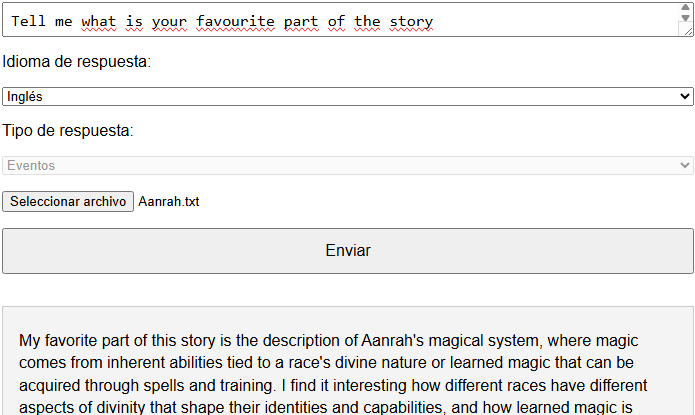
\includegraphics[width=1\textwidth]{./Figures/promp-testing.png}
	\caption{Prueba de desconexión del módulo generador de instrucciones.}
	\label{fig:prompt-test}
\end{figure}

\subsection{Resultados de \textit{deepseek}}
En el caso de \textit{deepseek}, presentó una adaptación al contexto narrativo aceptable y se ciñó correctamente al
tipo de elemento narrativo que se especificó.
No obstante, su desempeño en relación con la variedad de las ideas fue bajo al presentar puntos muy similares entre sí.
Este problema fue especialmente notable en el caso de los personajes y eventos.
Por último, la consistencia de sus respuestas varió en ocasiones.
Esto significa que su sensibilidad a la temperatura es bastante alta.
El modelo puede responder en español, pero los errores de traducción y alucinaciones son frecuentes,
tal y como se muestra en la figura \ref{fig:deepseek-esp}:

\begin{figure}[htbp]
	\centering
	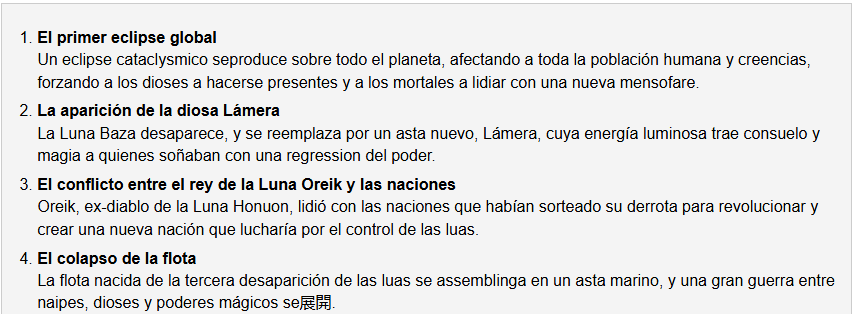
\includegraphics[width=1\textwidth]{./Figures/deepseek-noprompt-spanish.png}
	\caption{Resultado en español de \textit{deepseek} para eventos.}
	\label{fig:deepseek-esp}
\end{figure}
\pagebreak
\subsection{Resultados de \textit{mistral}}
El modelo generalista de \textit{mistral} no consiguió la misma calidad en sus respuestas.
Las propuestas, aunque tienen relación con el contexto de la historia,
muestran una conexión sin demasiada profundidad en los detalles ni en su variedad.
En los casos de geografía y asentamientos, su relación con el contexto es mínima o nula
(ver figura \ref{fig:mistral-geo}), lo que sugiere que su entrenamiento no le permite ser
flexible en la generación de contenido narrativo sin instrucciones previas.
Este modelo pierde completamente el contexto al responder en español,
lo que provoca que utilice referencias reales,
como ciudades de Estados Unidos, personajes históricos o festividades internacionales.

\begin{figure}[htbp]
	\centering
	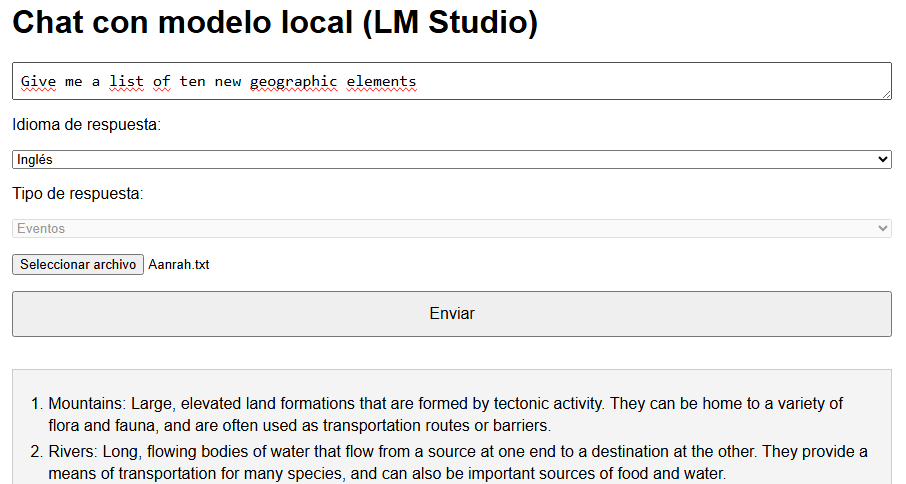
\includegraphics[width=1\textwidth]{./Figures/mistral-noprompt-geography.png}
	\caption{Resultado de \textit{mistral} para geografía}
	\label{fig:mistral-geo}
\end{figure}

%----------------------------------------------------------------------------------------
%	SECTION 6
%----------------------------------------------------------------------------------------
\section{Pruebas con modelos reentrenados y \textit{prompting} poco preciso}
Análogamente a la sección anterior, se llevaron a cabo pruebas equivalentes
sobre los modelos refinados con el fin de evaluar su rendimiento.
Los resultados permiten establecer una comparación entre estos LLM
y los modelos generalistas.

\subsection{Resultados de \textit{writing-roleplay}}
El modelo de \textit{writing-roleplay} funcionó correctamente en la generación de eventos,
comprendiendo adecuadamente el contexto y ofreciendo ideas interesantes.
Sin embargo, presentó problemas en el resto de elementos narrativos.
A pesar de que aporta una variedad aceptable y una ambientación de fantasía correcta,
su respuesta se ajusta más a un contenido predefinido que a algo adaptado a la ambientación
narrativa del fichero adjunto.
Finalmente, fue notoria la inconsistencia del modelo a la temperatura a la que fue configurado,
ya que ocasionalmente repetía información en vez de aportar ideas nuevas.

\subsection{Resultados de \textit{worldbuilder}}
En el caso de \textit{worldbuilder},
su comprensión de la entrada destacó sobre las alternativas generalistas,
aportando ideas con una relación profunda con el contexto de entrada
(Figura \ref{fig:worldbuilder-settle}).
Sin embargo, el modelo también tiene una sensibilidad alta a la temperatura
y ocasionalmente puede ignorar la ambientación al generar nuevo contenido.
Algo único de este LLM es que puede llegar a dar consejos al usuario de cómo
hacer la construcción de mundos, con diversas técnicas y explicaciones,
en vez de dar una lista de nuevas ideas.
También es el único que no puede dar respuestas en español.

\begin{figure}[htbp]
	\centering
	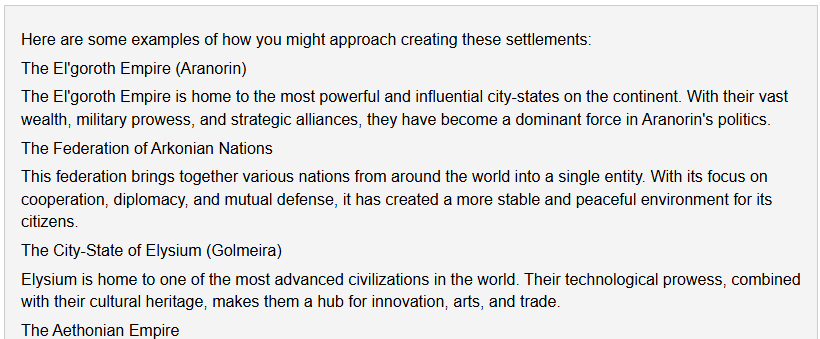
\includegraphics[width=1\textwidth]{./Figures/worldbuilder-noprompt-settlements.png}
	\caption{Resultado de \textit{worldbuilder} para asentamientos}
	\label{fig:worldbuilder-settle}
\end{figure}

\subsection{Resultados de \textit{arliai-rpmax}}
Finalmente, el modelo \textit{arliai-rpmax} fue el que mejor desempeño demostró. 
Se ajustó al contexto de entrada y profundizó en las respuestas de forma aceptable.
Donde también destacó es en la capacidad de generar texto en español sin verse afectado
en la calidad del mensaje. 

A nivel global, todos los LLM funcionaron bien para los eventos y las localizaciones,
mientras que carecieron de originalidad en la generación de personajes y geografía.
En la figura \ref{fig:rpmax-chars} se muestra un ejemplo de este fenómeno.

\begin{figure}[htbp]
	\centering
	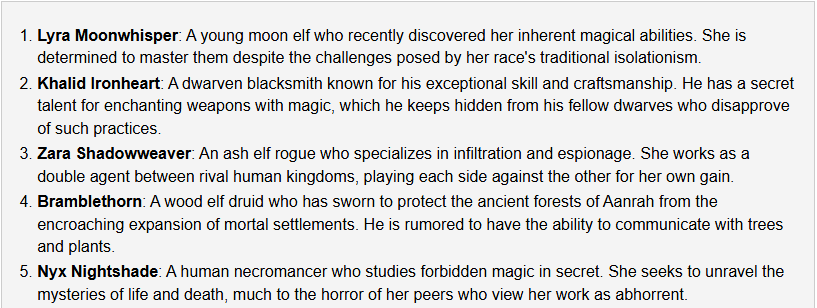
\includegraphics[width=1\textwidth]{./Figures/rpmax-noprompt-chars.png}
	\caption{Resultado de \textit{arliai-rpmax} para personajes}
	\label{fig:rpmax-chars}
\end{figure}

%----------------------------------------------------------------------------------------
%	SECTION 7
%----------------------------------------------------------------------------------------
\section{Pruebas con modelos generalistas y \textit{prompting} preciso}
Esta sección examina el rendimiento de modelos generalistas que no han sido específicamente
ajustados para tareas de ambientación narrativa.
A diferencia de enfoques anteriores sin refinamiento,
el objetivo aquí es maximizar la capacidad intrínseca del modelo mediante instrucciones detalladas,
buscando determinar la eficacia de esta técnica al trabajar con modelos accesibles públicamente.

Para ello, se hace uso del módulo de instrucciones y la interfaz \textit{web}
en su versión final. Tal y como se demuestra en la figura \ref{fig:full-prompt-test},
el sistema construye la instrucción de forma transparente para el usuario, por lo que
solo es necesario que se adjunte el fichero con el contexto narrativo.

\begin{figure}[htbp]
	\centering
	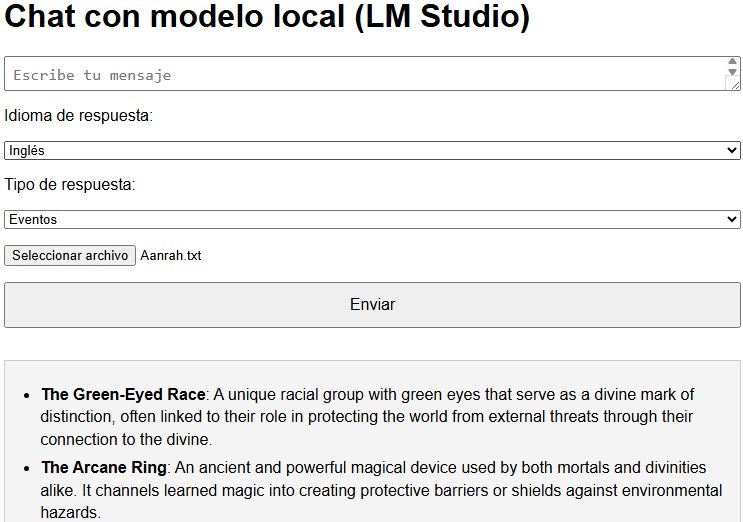
\includegraphics[width=0.85\textwidth]{./Figures/full-promp-testing.png}
	\caption{Prueba de la versión definitiva del sistema.}
	\label{fig:full-prompt-test}
\end{figure}

\subsection{Resultados de \textit{deepseek}}
Este modelo experimentó una mejora sustancial en la calidad de sus respuestas, tanto en la profundidad
contextual como en la variedad de las ideas que aporta.
La capacidad del modelo para relacionar elementos de la ambientación narrativa y
plasmarlos en las propuestas se vio significativamente potenciada, abarcando eventos, personajes y geografía
(ver figura \ref{fig:deepseek-prompt-char}).
La consistencia de las respuestas se mantuvo estable,
reduciéndose notablemente la aparición de errores de formato y temática.
Asimismo, el rendimiento en español mejoró, reduciendo el coste de la traducción.

\begin{figure}[htbp]
	\centering
	\includegraphics[width=1\textwidth]{./Figures/deepseek-prompt-characters.png}
	\caption{Resultado de \textit{deepseek} para personajes.}
	\label{fig:deepseek-prompt-char}
\end{figure}
\pagebreak
\subsection{Resultados de \textit{mistral}}
\textit{Mistral} mostró una adaptación inconsistente a la ingeniería de instrucciones precisas,
lo que se tradujo en una alta variabilidad en sus respuestas.
Aunque en algunos casos interpretó correctamente las directrices,
mostrando una ligera mejora respecto a las instrucciones básicas,
los errores fueron frecuentes. Entre los más comunes se incluyen la duplicación de la lista generada y
una pérdida considerable de la temática en la respuesta. Esto a menudo resultaba en la generación de más de los 10 elementos especificados por defecto,
con una relación mínima o nula con el contexto general.
Además, el modelo perdió por completo su capacidad de generar respuestas en español bajo esta configuración.

\begin{figure}[htbp]
	\centering
	\includegraphics[width=1\textwidth]{./Figures/mistral-prompt-locations.png}
	\caption{Resultado de \textit{mistral} para localizaciones.}
	\label{fig:mistral-prompt-locations}
\end{figure}

%----------------------------------------------------------------------------------------
%	SECTION 8
%----------------------------------------------------------------------------------------
\section{Pruebas con modelos reentrenados y \textit{prompting} preciso}
Esta sección presenta y analiza los resultados obtenidos de las pruebas realizadas sobre los modelos refinados,
empleando esta vez instrucciones precisas.

\subsection{Resultados de \textit{writing-roleplay}}
La comprensión del LLM experimentó una ligera mejora,
siendo esta más evidente en la generación de eventos.
Sin embargo, en el resto de categorías, el rendimiento se mantuvo similar al observado con \textit{prompting} poco preciso.
En varias ocasiones, el modelo interpretó que debía generar una lista de varias decenas de puntos,
lo que provocó bloqueos en el sistema, indicando una posible sobrecarga o un fallo en el manejo de la longitud de la respuesta esperada.

\begin{figure}[htbp]
	\centering
	\includegraphics[width=1\textwidth]{./Figures/writing-prompt-geography.png}
	\caption{Alucinación de \textit{writing-roleplay} para geografía.}
	\label{fig:writing-geography}
\end{figure}

\subsection{Resultados de \textit{worldbuilder}}
Con la aplicación de las nuevas instrucciones, el modelo mostró
una mejora perceptible en la comprensión del contexto de entrada,
lo cual se reflejó en la calidad de la generación.
No obstante, en los apartados de geografía y localizaciones, no se observó una mejora significativa.
En esta configuración, también se registraron alucinaciones, como se ilustra en la figura \ref{fig:worldbuilder-hallucination},
que complejizaron el listado y llevaron a la devolución de varias listas con diferentes categorías,
sugiriendo nuevamente una tendencia a desviarse de la estructura de respuesta esperada.

\begin{figure}[htbp]
	\centering
	\includegraphics[width=1\textwidth]{./Figures/worldbuilder-hallucination-events.png}
	\caption{Alucinación de \textit{worldbuilder} en la generación de eventos.}
	\label{fig:worldbuilder-hallucination}
\end{figure}

\subsection{Resultados de \textit{arliai-rpmax}}
Gracias al refinamiento de los \textit{prompts},
este modelo mejoró significativamente su comprensión e inclusión del contexto,
lo que resultó en respuestas de calidad excepcional.
Además, \textit{arliai-rpmax} destacó por su robusta capacidad de generar texto en español,
manteniendo una calidad constante en el mensaje sin degradación.

\begin{figure}[htbp]
	\centering
	\includegraphics[width=1\textwidth]{./Figures/rpmax-prompt-events.png}
	\caption{Resultado de \textit{arliai-rpmax} en la generación de eventos.}
	\label{fig:rpmax-events}
\end{figure}

A nivel global, se observó una mejora consistente en la generación de eventos por parte de todos los LLM,
en comparación con las evaluaciones previas.
Sin embargo, los resultados no fueron tan favorables en la creación de personajes,
la geografía y las localizaciones,
donde los modelos continuaron exhibiendo limitaciones en originalidad y variedad.
Este fenómeno plantea la necesidad de investigar si se debe a un posible sobreentrenamiento en ciertas categorías
o a una escasez de información contextual relevante en la ambientación narrativa empleada en los ensayos.

%----------------------------------------------------------------------------------------
%	SECTION 9
%----------------------------------------------------------------------------------------
\section{Interpretación de resultados}
Previo al análisis global del rendimiento del sistema,
se han confeccionado dos grillas resumen que muestran cómo ha funcionado
cada combinación de modelo y estrategia de instrucciones a lo largo de la experimentación.
En ella, cada celda contiene una valoración del 1 al 5,
donde 1 indica un desempeño insuficiente y 5 refleja una ejecución excelente.
Esta síntesis numérica de las tablas \ref{tab:results-noprompt} y \ref{tab:results-prompt}
permite identificar patrones de mejora derivados
de intervenciones específicas, como la optimización de los \textit{prompts},
y facilita una evaluación comparativa entre configuraciones.
 
\begin{table}[h]
\centering
\caption{Tabla resumen de los ensayos con \textit{prompting} poco preciso.}
\resizebox{\textwidth}{!}{%
\begin{tabular}{l c c c c c c c c}
\toprule
\textbf{Modelo} & \textbf{Eventos} & \textbf{Personajes} & \textbf{Geografía} & \textbf{Localizaciones} & \textbf{Contexto} & \textbf{Temática} & \textbf{Originalidad} & \textbf{Consistencia} \\
\midrule
\texttt{deepseek} & 3 & 2 & 3 & 3 & 3 & 4 & 3 & 2 \\
\texttt{mistral} & 1 & 2 & 3 & 3 & 2 & 3 & 2 & 4 \\
\texttt{writing-roleplay} & 3 & 2 & 3 & 3 & 2 & 4 & 3 & 3 \\
\texttt{worldbuilder} & 4 & 3 & 3 & 3 & 3 & 4 & 4 & 3 \\
\texttt{arliai-rpmax} & 4 & 4 & 3 & 3 & 3 & 4 & 3 & 3 \\
\bottomrule
\end{tabular}%
}
\label{tab:results-noprompt}
\end{table}

\begin{table}[h]
\centering
\caption{Tabla resumen de los ensayos con \textit{prompting} preciso.}
\resizebox{\textwidth}{!}{%
\begin{tabular}{l c c c c c c c c}
\toprule
\textbf{Modelo} & \textbf{Eventos} & \textbf{Personajes} & \textbf{Geografía} & \textbf{Localizaciones} & \textbf{Contexto} & \textbf{Temática} & \textbf{Originalidad} & \textbf{Consistencia} \\
\midrule
\texttt{deepseek} & 4 & 3 & 4 & 3 & 4 & 3 & 4 & 3 \\
\texttt{mistral} & 2 & 2 & 3 & 3 & 3 & 3 & 3 & 2 \\
\texttt{writing-roleplay} & 4 & 3 & 2 & 2 & 3 & 3 & 3 & 2 \\
\texttt{worldbuilder} & 4 & 4 & 3 & 3 & 4 & 4 & 4 & 3 \\
\texttt{arliai-rpmax} & \textbf{5} & 4 & 3 & 3 & 4 & 4 & 4 & 4 \\
\bottomrule
\end{tabular}%
}
\label{tab:results-prompt}
\end{table}

\pagebreak
Teniendo en cuenta las puntuaciones, se pueden sacar las siguientes conclusiones:

\begin{itemize}
\item Los modelos generalistas tienen un rendimiento menor que aquellos LLM
	  que han sido reentrenados para la generación de contenido narrativo.
\item Es muy importante realizar una configuración de temperatura específica
      en cada modelo para limitar la aleatoriedad de la estructura de las respuestas.
\item Todos los modelos presentaron rigidez en la creación de algunos elementos narrativos,
	  posiblemente por requerir un mayor nivel de creatividad o por no tener suficiente contexto previo.
\item La estrategia de instrucciones desarrollada mejora notablemente la capacidad de profundizar en el
      contexto de entrada y plasmarlo en la salida, a costa de aumentar su inestabilidad en algunos casos.
\end{itemize}

Durante las pruebas se encontraron los siguientes errores con una frecuencia o gravedad considerables:
\begin{itemize}
\item Error de formato:
	  aunque no se trata de un problema con un impacto notable,
	  el formato de la salida de texto variaba en cada ejecución.
	  A veces empleaba listas de puntos, otras veces listas numeradas y, en raras ocasiones,
	  ignoró el formato y lo separó en párrafos.
	  Se estudió la posibilidad de forzar la salida de forma estructurada, pero los modelos no
	  respondieron positivamente al cambio, por lo que se concluyó que se implementará en trabajos futuros.
\item Tendencia de los LLM a generar preámbulo y resumen final:
      relacionado con el punto anterior,
	  algunos modelos tenían la tendencia de añadir información adicional alrededor de la lista de ideas.
	  En muchos de los casos, parafraseando las instrucciones recibidas por el módulo de instrucciones.
\item Errores de traducción: la mayoría de los modelos empeoraron su rendimiento al forzar su salida de 
      texto en español. Esto puede mitigarse integrando un modelo \textit{encoder} especializado en traducción
	  que actúe como etapa previa y posterior al modelo generador.
\item Procesamiento ``infinito'' de las peticiones:
	  aunque ocurrió en contadas ocasiones, este fenómeno provocaba que los modelos se quedaran
	  generando un texto demasiado largo, lo que hacía que su tiempo de respuesta aumentara
	  de unos pocos segundos a varios minutos, dando a entender que el sistema se había quedado bloqueado.
	  Este problema se puede mitigar mostrando este proceso de acumulación de palabras en tiempo real
	  o forzando su finalización tras alcanzar un tiempo o extensión configurable.
\end{itemize}
 
	% Chapter Template

\chapter{Conclusiones} % Main chapter title
En este capítulo final se engloban las conclusiones más relevantes del trabajo realizado
y se presentan posibles líneas de mejora de la solución alcanzada.

%----------------------------------------------------------------------------------------
%	SECTION 1
%----------------------------------------------------------------------------------------

\section{Conclusiones generales}

Tras el desarrollo del presente trabajo se pueden alcanzar las siguientes conclusiones:

\begin{itemize}
\item Los requerimientos de la planificacion del proyecto fueron alcanzados
      satisfactoriamente.
      El prototipo desarrollado supone un buen punto de partida para el estudio de
      la inclusión de la inteligencia artificial generativa como servicios para
      los usuarios que utilizan la \textit{app} de Critical Match.
      Además, la correcta separación de módulos permite al cliente ampliar el desarrollo
      de forma simple y efectiva.
      Por ultimo, los requerimientos de privacidad, propiedad intelectual y restricciones legales
      quedan amparadas por un módulo de modelos extensos de lenguaje que puede ser operado
      de forma local y sin conexión de internet.     
\item Hubo un retraso considerable en los tiempos estimados del proyecto debido a
      circunstancias académicas, personales y de \textit{hardware}.
      Sin embargo, ese tiempo de diseño y desarrollo adicional permitió alcanzar un sistema
      notablemente superior al diseñado en las primeras fases del proyecto. 
      A consecuencia de esto, muchas tareas fueron simplificadas y se alcanzó una flexibilidad
      en el sistema ideal para un prototipo.
\item Los riesgos relacionados con la capacidad de computación y los retrasos en el proyecto
      se materializaron con la severidad prevista.
      Aunque no comprometieron el éxito del proyecto,
      sí afectaron de forma significativa el plazo para su finalización.
\item Se resalta el valor práctico de la herramienta LM Studio,
      la cual no solo ha simplificado muchas de las tareas clave del proyecto,
      sino que también contribuye significativamente a la viabilidad de desarrollos futuros.
      El uso de servidores de este tipo resulta fundamental en un contexto donde
      la evolución de los modelos de lenguaje se encuentra en una situación de constantes cambios.
\end{itemize}
%----------------------------------------------------------------------------------------
%	SECTION 2
%----------------------------------------------------------------------------------------
\section{Próximos pasos}
Al ser un prototipo, el proyecto ofrece un amplio margen para futuras ampliaciones.
Se presentan a continuación algunas direcciones posibles:

\begin{itemize}
\item Interfaz \text{web}:
      aunque no está diseñado para un uso directo por parte de usuarios finales,
      es posible incorporar campos como la temperatura o la selección del modelo
      al que se desea realizar la petición, especialmente si el sistema se despliega
      en una máquina capaz de alojar múltiples modelos en paralelo.
\item Creación y entrenamiento fino de un LLM propio:
      desarrollar un modelo propio y ajustarlo mediante \textit{fine-tuning}
      permitiría adaptarlo de forma precisa al dominio narrativo,
      los estilos de respuesta deseados y las necesidades específicas del sistema,
      mejorando la coherencia, la creatividad o la eficiencia computacional.
      Para lograr esto será necesario contar con un banco de datos considerable y la
      implementación de análisis de datos.
\item Implementación de \textit{Mixture of Experts}:
      si se cuenta con la infraestructura que permita la ejecución de varios LLM en paralelo,
      integrar una arquitectura basada en mezcla de expertos permitiría distribuir
      la carga entre modelos especializados.
      Esto aumentaría la eficiencia del sistema y permitiría
      respuestas más ajustadas dependiendo del tipo de contenido solicitado.
\item Implementación de \text{structured output}:
      adoptar salidas estructuradas en lugar de texto libre 
      facilitaría la integración con otros sistemas
      y permitiría una validación automática del contenido generado,
      además de estructurar los mensajes de respuesta de forma unequívoca.
      LM Studio permite añadir esquemas JSON para la salida estructurada de los modelos,
      por lo que solo requeriría el uso de LLMs compatibles y una ingeniería debe
      instrucciones adecuada.
\item Uso de RAGs:
      la incorporación de sistemas de generación aumentada por recuperación
      permitiría enriquecer las respuestas generadas mediante la consulta de
      fuentes externas o bases de conocimiento previas.
      Esto puede mejorar la precisión factual, la consistencia del mundo narrativo
      y la personalización en tiempo real.
      Para operar un RAG es fundamental contar con una base de datos bien estructurado
      y con un volumen de datos considerable.
\end{itemize}

En definitiva, las propuestas aquí expuestas ofrecen un camino claro para potenciar
y consolidar la solución desarrollada.
La implementación de estas mejoras no solo ampliará las capacidades técnicas del sistema,
sino que también permitirá una mayor adaptabilidad a diferentes contextos
y necesidades narrativas.
De este modo, el prototipo podrá evolucionar hacia una herramienta robusta y versátil,
capaz de ofrecer respuestas más precisas, coherentes y personalizadas en futuros proyectos. 
\end{verbatim}

Los apéndices también deben escribirse en archivos .tex separados, que se deben ubicar dentro de la carpeta \emph{Appendices}. Los apéndices vienen comentados por defecto con el caracter \code{\%} y para incluirlos simplemente se debe eliminar dicho caracter.

Finalmente, se encuentra el código para incluir la bibliografía en el documento final.  Este código tampoco debe modificarse. La metodología para trabajar las referencias bibliográficas se desarrolla en la sección \ref{sec:biblio}.
%----------------------------------------------------------------------------------------

\section{Bibliografía}
\label{sec:biblio}

Las opciones de formato de la bibliografía se controlan a través del paquete de latex \option{biblatex} que se incluye en la memoria en el archivo memoria.tex.  Estas opciones determinan cómo se generan las citas bibliográficas en el cuerpo del documento y cómo se genera la bibliografía al final de la memoria.

En el preámbulo se puede encontrar el código que incluye el paquete biblatex, que no requiere ninguna modificación del usuario de la plantilla, y que contiene las siguientes opciones:

\begin{lstlisting}
\usepackage[backend=bibtex,
	natbib=true, 
	style=numeric, 
	sorting=none]
{biblatex}
\end{lstlisting}

En el archivo \file{reference.bib} se encuentran las referencias bibliográficas que se pueden citar en el documento.  Para incorporar una nueva cita al documento lo primero es agregarla en este archivo con todos los campos necesario.  Todas las entradas bibliográficas comienzan con $@$ y una palabra que define el formato de la entrada.  Para cada formato existen campos obligatorios que deben completarse. No importa el orden en que las entradas estén definidas en el archivo .bib.  Tampoco es importante el orden en que estén definidos los campos de una entrada bibliográfica. A continuación se muestran algunos ejemplos:

\begin{lstlisting}
@ARTICLE{ARTICLE:1,
    AUTHOR="John Doe",
    TITLE="Title",
    JOURNAL="Journal",
    YEAR="2017",
}
\end{lstlisting}


\begin{lstlisting}
@BOOK{BOOK:1,
    AUTHOR="John Doe",
    TITLE="The Book without Title",
    PUBLISHER="Dummy Publisher",
    YEAR="2100",
}
\end{lstlisting}


\begin{lstlisting}
@INBOOK{BOOK:2,
    AUTHOR="John Doe",
    TITLE="The Book without Title",
    PUBLISHER="Dummy Publisher",
    YEAR="2100",
    PAGES="100-200",
}
\end{lstlisting}


\begin{lstlisting}
@MISC{WEBSITE:1,
    HOWPUBLISHED = "\url{http://example.com}",
    AUTHOR = "Intel",
    TITLE = "Example Website",
    MONTH = "12",
    YEAR = "1988",
    URLDATE = {2012-11-26}
}
\end{lstlisting}

Se debe notar que los nombres \emph{ARTICLE:1}, \emph{BOOK:1}, \emph{BOOK:2} y \emph{WEBSITE:1} son nombres de fantasía que le sirve al autor del documento para identificar la entrada. En este sentido, se podrían reemplazar por cualquier otro nombre.  Tampoco es necesario poner : seguido de un número, en los ejemplos sólo se incluye como un posible estilo para identificar las entradas.

La entradas se citan en el documento con el comando: 

\begin{verbatim}
\citep{nombre_de_la_entrada}
\end{verbatim}

Y cuando se usan, se muestran así: \citep{ARTICLE:1}, \citep{BOOK:1}, \citep{BOOK:2}, \citep{WEBSITE:1}.  Notar cómo se conforma la sección Bibliografía al final del documento.

Finalmente y como se mencionó en la subsección \ref{subsec:configurando}, para actualizar las referencias bibliográficas tanto en la sección bibliografía como las citas en el cuerpo del documento, se deben ejecutar las herramientas de compilación PDFLaTeX, BibTeX, PDFLaTeX, PDFLaTeX, en ese orden.  Este procedimiento debería resolver cualquier mensaje "Citation xxxxx on page x undefined".

	\chapter{Introducción específica} % Main chapter title

\label{Chapter2}

%----------------------------------------------------------------------------------------
%	SECTION 1
%----------------------------------------------------------------------------------------
En este capítulo se profundiza en aquellos aspectos clave para el desarrollo de este trabajo.
En primer lugar, se presentan los requerimientos de sistema y se amplía la información acerca de los modelos de 
inteligencia artificial que se han utilizado.
Finalmente, se expone el conjunto de técnicas y herramientas que se han aplicado a dichos modelos.

\section{Requerimientos del sistema}
Para llevar a cabo este trabajo
se identificaron una serie de requerimientos fundamentales.
A continuación se listan aquellos que están directamente relacionados con la implementación:

\begin{enumerate}
	\item Requerimientos del servidor:
	      \begin{enumerate}
		      \item El servidor debe alojar y administrar la información relativa al \textit{dataset} y la configuración del modelo LLM.
		      \item El servidor debe contar con los \textit{prompts} necesarios para especializar la respuesta de  la inteligencia artificial.
		      \item Al ser desplegado, el servidor deberá acceder al módulo LLM y utilizarlo en el procesamiento de peticiones entrantes.
		      \item El servidor debe dar acceso a clientes externos a través del protocolo API REST.
		      \item Los servicios REST deben aceptar entrada de texto en varios formatos: pdf, txt, docx o texto plano en el cuerpo de la petición.
		      \item Los servicios REST devolverán la respuesta en formato simple HTML para su cómoda visualización en un navegador.
		      \item El prototipo del servidor debe de tener una disponibilidad del 100\% durante la demostración.
	      \end{enumerate}
	\item Requerimientos del módulo LLM:
	      \begin{enumerate}
		      \item El módulo LLM debe aceptar entrada de texto y generar texto como salida.
		      \item En caso de que el texto de entrada sea legible, el módulo LLM debe aportar una respuesta con un detalle y profundidad razonables,
		            además de ser coherente con las instrucciones recibidas.
		      \item El módulo se ajustará a los \textit{prompts} recibidos para que, con el mismo contexto,
			  		devuelva información enfocada en un aspecto específico de la narrativa.
		      \item El tiempo de respuesta del módulo LLM debe estar en un rango de tiempo razonable para un servicio REST (no más de 5 minutos).
	      \end{enumerate}
\end{enumerate}

%----------------------------------------------------------------------------------------
%	SECTION 2
%----------------------------------------------------------------------------------------

\section{Modelos extensos de lenguaje}
Para abordar los requisitos de generación de texto resultó fundamental la utilización 
de modelos extensos de lenguaje, comúnmente denominados \textit{Large Language Models} (LLM).
Estos modelos son entrenados sobre enormes volúmenes de datos textuales para especializarlos
en predecir la secuencia de texto más probable dada una entrada previa.
Esta habilidad les permite generar texto de forma coherente con el contexto
al adaptarse al tono, estilo y contenido esperado.

Los LLM se basan en redes neuronales profundas que manejan miles de millones de parámetros
(lo que justifica su clasificación como modelos ``extensos'') para identificar patrones complejos del lenguaje natural \cite{att_is_all_you_need}. 
Estos modelos utilizan \textit{tokens} como unidad básica de texto en su procesamiento.
Los \textit{tokens} pueden representar palabras completas, fragmentos de palabras o signos de puntuación,
dependiendo del sistema de tokenización utilizado.
Estos \textit{tokens} se convierten posteriormente en vectores numéricos
mediante una capa de \textit{embedding} \cite{mikolov2013efficient}, que permite al modelo operar sobre ellos.

Los LLM modernos utilizan la arquitectura de \textit{transformers} \cite{att_is_all_you_need},
un tipo de red neuronal que permite procesar secuencias de texto en paralelo y asignar diferentes niveles de relevancia
(atención) a distintas partes del texto mediante un mecanismo llamado \textit{self-attention} \cite{att_is_all_you_need}.
Esta arquitectura supera notablemente a estructuras anteriores como \textit{Long-Short Term Memory} \cite{hochreiter1997long}
o \textit{Gated Recurrent Unit} \cite{cho2014learning} en cuestiones de eficiencia y rendimiento.

Además de su capacidad de paralelización y memoria a largo plazo, los LLM basados en \textit{transformers} operan 
mediante la predicción de la siguiente cadena de \textit{tokens} a partir del contexto previo.
En este proceso hay elementos que controlan la generación, entre los que se destaca la temperatura \cite{radford2019language}.
La temperatura regula la aleatoriedad de los \textit{tokens}: valores bajos tienden a generar respuestas deterministas,
mientras que valores altos proporcionan respuestas más diversas y creativas\footnote{
	Esto también aumenta las probabilidades de que esta respuesta sea incoherente, también llamada alucinación.
}. Existen otros parámetros que controlan la variedad del texto, por ejemplo \textit{top-k} y \textit{top-p} \cite{holtzman2019curious}.

A medida que los LLM aumentan en extensión de parámetros y profundidad de entrenamiento, empiezan a manifestar cualidades
que no fueron explícitamente programadas. Entre estas capacidades destacan el razonamiento en múltiples pasos,
traducción automática entre idiomas, capacidad de responder a preguntas complejas y generación creativa y coherente de texto
que va más allá de la simple predicción de cadenas de texto.

Por ejemplo, modelos como GPT-3 \cite{Brown2020GPT3} de OpenAI, PaLM \cite{chowdhery2022palm} de Google 
y LLaMA \cite{touvron2023llama} de Meta han demostrado un rendimiento notable
en multitud de tareas complejas como realizar inferencias lógicas, resolver problemas matemáticos,
resumir textos extensos y generar código a partir de descripciones en lenguaje natural.
Esto no solo amplía el espectro de aplicaciones prácticas de los LLM,
sino que también plantea nuevas líneas de investigación para comprender cómo el tamaño y
la calidad del entrenamiento impactan en la adquisición de habilidades cognitivas sofisticadas.

%----------------------------------------------------------------------------------------
%	SECTION 3
%----------------------------------------------------------------------------------------

\section{Ingeniería de \textit{prompts}}
La ingeniería de \textit{prompts} (\textit{prompt engineering}) es una técnica fundamental en la optimización de la salida de los modelos extensos de lenguaje
que se basa en guiar el proceso de razonamiento del modelo hacia un objetivo específico a través de un conjunto de entradas textuales.
A diferencia de la programación tradicional, que se expresa de forma explícita la lógica mediante el uso de código en un lenguaje de programación,
el comportamiento de los LLM se guía mediante lenguaje natural.

Esta técnica ha emergido como una nueva disciplina en la que intervienen conceptos linguísticos y computacionales.
La forma en la que se redacta una instrucción puede influir de forma notable en la coherencia, relevancia, creatividad
y precisión de las respuestas.

Entre las estrategias comunes de ingeniería de prompts se encuentran \textit{zero/few-shot prompting} \cite{brown2020language}\cite{kojima2022large},
que emplea ejemplos en el \textit{prompt} para guiar la generación; \textit{chain of thought prompting} \cite{wei2022chain} invita al modelo a razonar explícitamente
los pasos intermedios antes de llegar a la conclusión; o \textit{prompt chaining} \cite{promptchaining2023} que invita al modelo a realizar un análisis previo
sobre el contexto o instrucciones para enfocar la salida.
En la figura \ref{fig:prompting} se ilustra cómo estas estrategias de instrucción afectan directamente la salida generada por el modelo.
Cabe destacar que las distintas técnicas de \textit{prompting} descritas no son excluyentes entre sí,
sino que pueden combinarse de manera complementaria, lo que potencia la capacidad de razonamiento
y la precisión de los LLM en tareas complejas.
% \footnote{
% 	Imagen obtenida del material del curso de especializacion en inteligencia artificial de la FIUBA,
% 	materia de \textit{LLM} \cite{fiubaPrompt} 
% 	}
\begin{figure}[htbp]
	\centering
	\includegraphics[width=0.9\textwidth]{./Figures/prompting.png}
	\caption{Ejemplo de uso de técnicas de \textit{prompting}.}
	\label{fig:prompting}
\end{figure}

A su vez, la ingeniería de \textit{prompts} ha demostrado ser fundamental en aquellos contextos en los que
el \textit{fine-tuning} no es viable, ya que hay muchos modelos cerrados que solo son accesibles a través de una API
y la capacidad de modificar su comportamiento sin reentrenamiento se vuelve crucial.
Por lo tanto, esta técnica se convierte en una herramienta práctica, eficiente y cada vez más sofisticada
para adaptar modelos generalistas a tareas específicas.

%----------------------------------------------------------------------------------------
%	SECTION 4
%----------------------------------------------------------------------------------------

\section{Ajuste fino}
El ajuste fino (\textit{fine-tuning}) \cite{howard2018universal} es una técnica de entrenamiento de modelos extensos de lenguaje 
que permite adaptar un modelo previamente entrenado a una tarea en específico.
A diferencia del entrenamiento desde cero, esta técnica parte de una base
y lo especializa utilizando un conjunto mucho más pequeño y específico de datos.
De este modo se reduce significativamente el coste computacional a la vez que se aprovecha
la capacidad predictiva del modelo del que se parte.

Para llevar a cabo el ajuste fino, se conservan la estructura y los parámetros previamente entrenados del modelo base,
evitando así la necesidad de un entrenamiento completo desde cero.
En la práctica, el proceso de \textit{fine-tuning} suele centrarse en modificar únicamente una parte reducida del modelo,
como las capas superiores, que son las más cercanas a la salida y, por tanto,
más fácilmente adaptables a tareas específicas.
Alternativamente, pueden integrarse nuevas capas que se entrenan sin alterar el resto del modelo.
Esta aproximación permite preservar los conocimientos generales adquiridos durante el preentrenamiento
mientras se optimiza la capacidad del modelo para tareas concretas.

Además, en escenarios con recursos computacionales limitados
se utilizan técnicas de ajuste fino eficiente (parameter-efficient fine-tuning, PEFT),
como LoRA (\textit{Low-Rank Adaptation}) \cite{hu2021lora},
\textit{prefix tuning} \cite{li2021prefix} o \textit{prompt tuning}.
Estas estrategias reducen la cantidad de parámetros que deben entrenarse,
lo que no solo disminuye el tiempo de ajuste y el consumo de memoria,
sino que también facilita la reutilización del modelo base en múltiples contextos sin interferencia entre tareas.

Al adaptar un modelo generalista a contextos específicos,
se logra una mejora sustancial en la precisión, relevancia y
sensibilidad del modelo frente a matices del lenguaje propios del área de aplicación.
No obstante, es fundamental contar con datos de alta calidad y
bien etiquetados para evitar la sobreespecialización o la introducción de sesgos.

\pagebreak
%----------------------------------------------------------------------------------------
%	SECTION 5
%----------------------------------------------------------------------------------------
\section{LM Studio y otras tecnologías}
LM Studio \cite{lmstudio} es una plataforma de código abierto diseñada para facilitar la interacción
y despliegue de modelos extensos de lenguaje (LLM) de manera local,
lo que permite a los usuarios ejecutar y experimentar con modelos sin depender de servicios en la nube.
Esta herramienta destaca por su integración sencilla, soporte para múltiples formatos de modelos y una interfaz amigable.

Una de las ventajas clave de LM Studio es su capacidad para manejar modelos grandes y complejos con eficiencia.
Ofrece funcionalidades como la gestión de memoria optimizada,
soporte para cuantización y carga progresiva de modelos
lo que permite que usuarios con recursos limitados puedan aprovechar la potencia de los LLM
sin necesidad de infraestructura costosa.
Además, LM Studio facilita la personalización de modelos mediante interfaces accesibles,
lo que la convierte en una opción popular tanto para investigadores como para desarrolladores
que desean incorporar inteligencia artificial avanzada en sus proyectos.

Para la implementación del \textit{backend} de la aplicación que interactúa con LM Studio, se utilizó \textit{Python},
un lenguaje de programación ampliamente adoptado en el ámbito de la inteligencia artificial por su simplicidad
y la gran cantidad de bibliotecas disponibles.
Se empleó la biblioteca de FastAPI \cite{fastapi} en al construcción del servidor web gracias a su sintaxis intuitiva,
lo que facilitó la creación de \textit{endpoints} eficientes para la comunicación entre el usuario y el modelo.

Por otro lado, \textit{PyTorch} \cite{pytorch} es la biblioteca de referencia para el desarrollo 
y entrenamiento de modelos de aprendizaje profundo, incluyendo los LLM.
Proporciona una interfaz dinámica y flexible que permite tanto el entrenamiento
como la inferencia eficiente en hardware acelerado, y es compatible con múltiples plataformas. 
	\chapter{Diseño e implementación} % Main chapter title
\label{Chapter3} % Change X to a consecutive number; for referencing this chapter elsewhere, use \ref{ChapterX}
En este capítulo se detalla cómo se ha ejecutado la implementación del trabajo,
incluyendo la arquitectura del sistema, procesamiento de peticiones,
modelos extensos de lenguaje utilizados y las técnicas empleadas sobre la inteligencia artificial.
Adicionalmente, se incluyen los hallazgos intermedios significativos que fueron fundamentales para la implementación final.

\definecolor{mygreen}{rgb}{0,0.6,0}
\definecolor{mygray}{rgb}{0.5,0.5,0.5}
\definecolor{mymauve}{rgb}{0.58,0,0.82}

%%%%%%%%%%%%%%%%%%%%%%%%%%%%%%%%%%%%%%%%%%%%%%%%%%%%%%%%%%%%%%%%%%%%%%%%%%%%%
% parámetros para configurar el formato del código en los entornos lstlisting
%%%%%%%%%%%%%%%%%%%%%%%%%%%%%%%%%%%%%%%%%%%%%%%%%%%%%%%%%%%%%%%%%%%%%%%%%%%%%
\lstset{ %
  backgroundcolor=\color{white},   % choose the background color; you must add \usepackage{color} or \usepackage{xcolor}
  basicstyle=\footnotesize,        % the size of the fonts that are used for the code
  breakatwhitespace=false,         % sets if automatic breaks should only happen at whitespace
  breaklines=true,                 % sets automatic line breaking
  captionpos=b,                    % sets the caption-position to bottom
  commentstyle=\color{mygreen},    % comment style
  deletekeywords={...},            % if you want to delete keywords from the given language
  %escapeinside={\%*}{*)},          % if you want to add LaTeX within your code
  %extendedchars=true,              % lets you use non-ASCII characters; for 8-bits encodings only, does not work with UTF-8
  %frame=single,	                % adds a frame around the code
  keepspaces=true,                 % keeps spaces in text, useful for keeping indentation of code (possibly needs columns=flexible)
  keywordstyle=\color{blue},       % keyword style
  language=[ANSI]C,                % the language of the code
  %otherkeywords={*,...},           % if you want to add more keywords to the set
  numbers=left,                    % where to put the line-numbers; possible values are (none, left, right)
  numbersep=5pt,                   % how far the line-numbers are from the code
  numberstyle=\tiny\color{mygray}, % the style that is used for the line-numbers
  rulecolor=\color{black},         % if not set, the frame-color may be changed on line-breaks within not-black text (e.g. comments (green here))
  showspaces=false,                % show spaces everywhere adding particular underscores; it overrides 'showstringspaces'
  showstringspaces=false,          % underline spaces within strings only
  showtabs=false,                  % show tabs within strings adding particular underscores
  stepnumber=1,                    % the step between two line-numbers. If it's 1, each line will be numbered
  stringstyle=\color{mymauve},     % string literal style
  tabsize=2,	                   % sets default tabsize to 2 spaces
  title=\lstname,                  % show the filename of files included with \lstinputlisting; also try caption instead of title
  morecomment=[s]{/*}{*/}
}


%----------------------------------------------------------------------------------------
%	SECTION 1
%----------------------------------------------------------------------------------------
\section{Arquitectura del sistema}

Los primeros esfuerzos en el desarrollo del trabajo se enfocaron en definir el conjunto de módulos que compondrían la solución.
Estos componentes fueron identificados correctamente desde el principio:
un servidor \textit{web} y un módulo de modelos extensos de lenguaje.
Sin embargo, su relación en el sistema sí cambió durante la fase de implementación.

Inicialmente, durante la fase de diseño, se concibió que el servidor \textit{web} también alojaría el modelo extenso de lenguaje 
y sería responsable de gestionar su conjunto de datos, entrenamiento y despliegue.
Esta decisión se tomó al principio de la implementación,
influenciada por la forma en la que se trabaja con redes neuronales sencillas.
Hacer que esa arquitectura funcionase en este trabajo era mucho más complejo de lo estimado
por la propia naturaleza de los modelos extensos de lenguaje.
La incertidumbre generada por la ausencia de un conjunto de datos de calidad y tamaño suficientes,
y la dificultad implícita de reentrenar un modelo tan grande,
fueron un factor de riesgo permanente durante la fase de diseño.

Fue necesario profundizar en las materias de procesamiento de lenguaje natural y \textit{Large Language Models} \cite{fiubaLlm}
para definir una solución efectiva a este problema.
Finalmente se decidió por no solo ``extraer'' el módulo de modelos extensos de lenguaje del servidor \textit{web}
sino por simplificar su complejidad de programación haciendo uso de la herramienta LM Studio.
Este programa permite administrar los modelos locales de la computadora,
añadir nuevos a través de una interfaz de descarga
y hacer uso del hardware disponible para arrancarlos de forma transparente para el usuario.
Además, cuenta con varias ventanas de configuración de parámetros de lanzamiento del modelo, \textit{prompts} personalizados,
salida estructurada a través de un esquema JSON,
opciones relacionadas con la aleatoriedad y temperatura de la inferencia y otras características experimentales.

De este modo, el servidor \textit{web} también se simplificó en el desarrollo, ahorró mucho trabajo de programación sin
comprometer la calidad del proceso de la inteligencia artificial.
Esto también es coherente con la arquitectura de servidor ligero esperable en un prototipo
y tiene una mejor sinergia con bibliotecas orientadas al despliegue de servidores sencillos.

Tal y como se muestra en la figura \ref{fig:sist},
el prototipo es accesible para los clientes a través del protocolo HTTP-REST que expone el servidor.
Además, durante el desarrollo se implementó una sencilla página \text{web} para realizar peticiones de prueba
y mostrar la salida de texto obtenida.

\begin{figure}[htbp]
	\centering
	\includegraphics[width=0.9\textwidth]{./Figures/Sistema_es.png}
	\caption{Arquitectura del sistema.}
	\label{fig:sist}
\end{figure}

Otra ventaja de haber diseñado ambos módulos de forma independiente es que facilita al cliente
profundizar de forma paralela en los componentes sin comprometer el funcionamiento del resto del sistema.
Puede decidir si sustituir la implementación de uno u ambos módulos, escalarlos y distribuirlos en distintos entornos
para ajustarlo a su aplicación para \text{smartphones} y plan de expansión de servicios. 

%----------------------------------------------------------------------------------------
%	SECTION 2
%----------------------------------------------------------------------------------------
\section{Procesamiento de peticiones \textit{web} y ficheros}
Para la implementación del servidor web se decidió utilizar la biblioteca de FastAPI \cite{fastapi}.
Es una biblioteca moderna y de alto rendimiento para la construcción de APIs \text{web} en Python,
diseñada sobre estándares como OpenAPI \cite{openapi} y JSON schema.
Ofrece una forma rápida y eficiente de desarrollar interfaces REST
con una sintaxis sencilla y basada en anotaciones.
Esto permite una validación automática de datos de entrada y generación de documentación.
Todo esto hace que FastAPI sea una opción ideal para construir microservicios y prototipos rápidos.

El servidor expone dos servicios principales.
El primero es un \textit{endpoint} de tipo GET que proporciona la página \textit{web} que visualiza la interfaz gráfica del prototipo.
El otro servicio implementa un método POST para recibir las peticiones de consulta por parte del usuario para su procesamiento
y reenvío al módulo de inteligencia artificial. 


\pagebreak
\subsection{Procesamiento de peticiones}
En la figura \ref{fig:flux} se representa el diagrama de flujo correspondiente al manejo de las peticiones entrantes.

\begin{figure}[htbp]
	\centering
	\includegraphics[width=1\textwidth]{./Figures/flux-diagram.png}
	\caption{Diagrama de flujo del procesamiento de peticiones.}
	\label{fig:flux}
\end{figure}

El proceso comienza cuando el cliente envía una solicitud con los datos de consulta a través de un cliente REST.
Esto puede ser a través del formulario proporcionado por el servidor o a través de cualquier otra herramienta como,
por ejemplo, PostMan.
Tras realizar las comprobaciones iniciales,
el servidor continúa procesando la información mediante una serie de funciones específicas:
\begin{itemize}
\item \texttt{extract\_text\_from\_file}:
es el proceso encargado de extraer la información textual de los ficheros adjunto
y formatearlo para que el módulo de modelos extensos de lenguaje sea capaz de interpretarlo.
En esta función se hace uso de las bibliotecas de cgardet, docx y fitz para la detección del formato y
su conversión a texto plano.
\item \texttt{build\_prompt}:
esta función es la encargada de construir el \textit{prompt} a partir del texto extraído del fichero
y las entradas adicionales proporcionadas por el usuario, entre las que se incluyen el idioma de
la respuesta, el tipo de listado que se solicita y algunas instrucciones adicionales.
En esta función se emplea la ingeniería de \textit{prompting} que se envía posteriormente al módulo LLM.
Se detalla más adelante en la sección \ref{subsec:prompt}.
\item \texttt{clean\_and\_render\_markdown}:
esta función se encarga de limpiar la salida y formatearla en código HTML
a través de la biblioteca markdown para una mejor legibilidad en navegadores web.
\end{itemize}

Cabe destacar que para la comunicación con el módulo LLM,
aunque LM Studio ofrece un SDK en Python para interactuar mediante programación,
se optó por utilizar su interfaz REST.
La razón es que así el servidor \textit{web} no depende exclusivamente de la biblioteca de LM Studio.
Al emplear un protocolo de comunicación estándar como REST,
el servidor web puede interactuar fácilmente con cualquier otro servicio que aloje modelos extensos de lenguaje,
lo que le da mayor flexibilidad.

\subsection{Interfaz gráfica}
El servidor también facilita el acceso a una página \textit{web} con la interfaz gráfica del prototipo,
tal y como se aprecia en la figura \ref{fig:webPage}.

\begin{figure}[htbp]
	\centering
	\includegraphics[width=0.8\textwidth]{./Figures/webpage.png}
	\caption{Interfaz gráfica del prototipo.}
	\label{fig:webPage}
\end{figure}

El formulario consta de los siguientes elementos:
\begin{itemize}
\item Cuadro de texto:
este elemento se utiliza para darle las instrucciones específicas a la inteligencia artificial.
Está pensado para que sea un mensaje breve y conciso que pueda ayudar al usuario a guiar un poco mejor la respuesta.
Es un parámetro opcional y puede dejarse en blanco.
\item Idioma de respuesta:
se trata de un \textit{combobox} que contiene dos opciones: inglés y español.
El módulo LLM responderá en el idioma seleccionado, independientemente del idioma del fichero de entrada.
Este elemento se añadió porque algunos modelos presentan comportamientos anómalos si responden en un idioma distinto al inglés.
\item Tipo de respuesta:
permite a la inteligencia artificial centrar su respuesta en un aspecto concreto de la narrativa.
Al estar instruida en devolver listas de elementos, la idea es que el usuario pueda elegir la opción
específica de la creación de mundos que le interese.
\item Fichero adjunto:
es el elemento más importante del formulario.
El usuario puede agregar un fichero con el contexto narrativo existente
y enviarlo a la inteligencia artificial para que genere nuevo contenido.
\end{itemize}

%----------------------------------------------------------------------------------------
%	SECTION 3
%----------------------------------------------------------------------------------------
\section{Gestión de modelos extensos de lenguaje}
El siguiente paso en la fase de implementación fue la instalación
y configuración del módulo de modelos extensos de lenguaje.
Inicialmente, se analizó si la gestión y comunicación con la LLM se haría a través de una
API en la nube o alojarlo localmente en el servidor \textit{web}.

La opción de la API implicaba depender de servicios externos
en internet, lo que resultaba en peores tiempos de respuesta y un coste adicional significativo
debido a los modelos de pago por uso que restringen la cantidad de consultas.
A su vez, la interacción con servicios externos exponía la información transmitida en las consultas
lo que podría incumplir los requerimientos de protección de la privacidad
y propiedad intelectual de los datos del cliente.
También se observó un menor número de modelos disponibles y opciones de personalización,
lo que dificultaba la experimentación y adaptación de los LLM a las necesidades específicas del sistema.

Por otra parte, la opción de gestionar los modelos extensos de lenguaje
de forma nativa presentaba desafíos considerables.
Desarrollar la infraestructura \textit{software} necesaria para la gestión de modelos
era una tarea con alta complejidad técnica que iba más allá de la mera integración de \textit{frameworks}.
Esto podía suponer limitaciones significativas en el proceso de configuración de los modelos y,
en consecuencia, provocar un coste elevado en términos de tiempo y recursos de desarrollo.

Por estos motivos se decidió buscar alternativas para este módulo y se encontraron varias herramientas que
cumplían con las características deseadas, y las más llamativas fueron
Ollama \cite{ollama}, GPT4All \cite{gpt4all} y LM Studio \cite{lmstudio}.
Esta última fue la opción elegida eventualmente por su interfaz intuitiva y buscador de modelos,
además de simplificar la gestión y configuración de los LLM.
Alojar localmente los modelos permite el envío ilimitado de consultas
y cumple con los requisitos de privacidad de los datos del cliente.

En los siguientes apartados se detallan los distintos procesos de gestión que se llevaron a cabo con LM Studio.

\subsection{Descarga de modelos}
El menú \textit{discover} de LM Studio da acceso al explorador de modelos extensos de lenguaje,
permitiendo a los usuarios navegar por una vasta biblioteca alojada principalmente en la plataforma Hugging Face \cite{huggingface}.
Como se ilustra en la figura \ref{fig:downloadMenu},
esta herramienta de búsqueda facilita la localización de modelos específicos mediante filtros por nombre o palabras clave,
presentando los resultados en un listado que se ajusta a los criterios definidos.
Al seleccionar un modelo, se muestra una sección de detalles con sus características y las distintas opciones de descarga disponibles.

\begin{figure}[htbp]
	\centering
	\includegraphics[width=0.8 \textwidth]{./Figures/download_menu.png}
	\caption{Buscador de modelos de LM Studio.}
	\label{fig:downloadMenu}
\end{figure}

Esta herramienta se empleó para la búsqueda y descarga de múltiples modelos,
que se enumeran y detallan en la subsección \ref{subsec:modelos-llm}.
Se eligieron tanto modelos generalistas como aquellos especializados en \textit{roleplay},
con el fin de analizar y comparar su rendimiento en tareas de construcción de mundos.

\subsection{Administración y configuración de modelos}
LM Studio permite la gestión y configuración de los modelos locales en el menú \textit{My Models}.
Además de listar los LLM descargados en el equipo, esta ventana permite personalizar
sus parámetros de ejecución para optimizar el rendimiento y la precisión de las respuestas.

\pagebreak
Como se muestra en la figura \ref{fig:configMenu},
al seleccionar un modelo se tiene acceso a un conjunto de ajustes agrupados
en varios conjuntos.
Como se trabajó en el \textit{prompting} en el servidor \textit{web},
los esfuerzos de configuración se centraron en los parámetros de carga e inferencia.

\begin{figure}[htbp]
	\centering
	\includegraphics[width=0.8 \textwidth]{./Figures/config_menu.png}
	\caption{Configurador de modelos de LM Studio.}
	\label{fig:configMenu}
\end{figure}

La longitud del contexto resultó ser un parámetro fundamental en el trabajo.
Dado que las consultas de los usuarios se espera que vengan acompañadas de relatos extensos de \textit{worldbuilding},
era crucial que el LLM pudiera procesar y comprender grandes volúmenes de texto para generar respuestas coherentes y relevantes.
Los modelos tienen configurado por defecto un tamaño de contexto de 2048 o 4096 \textit{tokens},
un valor muy por debajo del tamaño de petición que se estima.

Para superar esta limitación, se seleccionó un tamaño de contexto compatible con las capacidades relativas de cada modelo,
a menudo indicado en los detalles.
Esta configuración fue esencial para asegurar que los LLM pudieran asimilar la totalidad de los relatos proporcionados.
Adicionalmente, se exploraron diversas tácticas para gestionar el exceso de contexto,
resultando más eficaces el acortamiento desde el principio de la secuencia o desde su punto medio.

Los parámetros de configuración de inferencia más importantes fueron la temperatura y
las técnicas de muestreo de probabilidad, como Top P o Top K.
Durante el desarrollo del proyecto, se observó que los valores predeterminados para estas variables
ya eran bastante adecuados. Por eso, solo fue necesario hacer ajustes mínimos en algunas de ellas.

Por defecto todos los modelos incluyen una sección de razonamiento.
Este parámetro fue deshabilitado en la configuración del modelo
y se filtró en el post-procesamiento para que no se mostrara en la respuesta al usuario.

\pagebreak
\subsection{Ejecución de modelos e interfaz REST}
La herramienta muestra y administra qué LLMs están activos y cargados en la memoria del sistema.
Además, también puede desplegar con un solo \textit{click} un servidor local compatible con la interfaz REST de OpenAI.
Cuando las peticiones llegan a este servidor, se registran en un log detallado que no solo proporciona
información sobre su estado sino que también muestra datos cruciales para la depuración de salidas incorrectas o errores.

\begin{figure}[htbp]
	\centering
	\includegraphics[width=1.0 \textwidth]{./Figures/developer_menu.png}
	\caption{Menú de desarrollador de LM Studio.}
	\label{fig:developerMenu}
\end{figure}

Una vez el modelo y el servidor están activos, el flujo del procesamiento de peticiones de la solución está completo.
El LLM, ya configurado con el tamaño de contexto ampliado y los parámetros de aleatoriedad ajustados,
gestiona la entrada, generando las respuestas esperadas.
Este diseño permite la misma forma de gestionar las peticiones,
sin importar el modelo que esté activo.

\pagebreak
\subsection{Modelos extensos de lenguaje utilizados}\label{subsec:modelos-llm}
El conjunto de modelos empleados en este trabajo se obtuvo a través de la herramienta de descarga de LM Studio.
Fueron seleccionados con un número de parámetros y un nivel de cuantización adecuado,
sin superar el límite de 12~GB de tamaño en memoria RAM dedicada en la tarjeta gráfica.
Esta parametrización permite aprovechar al máximo las capacidades del \textit{hardware} disponible,
con el objetivo de evaluar el rendimiento de distintos LLMs en tareas de generación narrativa.
En la tabla~\ref{tab:modelos_llm} se detallan las características de cada modelo:

\begin{table}[h]
\centering
\caption{Modelos extensos de lenguaje utilizados en el trabajo.}
\resizebox{\textwidth}{!}{%
\begin{tabular}{l l c c c r}
\toprule
\textbf{Modelo} & \textbf{Editor} & \textbf{Arquitectura} & \textbf{Parámetros} & \textbf{Cuantización} & \textbf{Tamaño (Contexto / VRAM)} \\
\midrule
\texttt{arliai-rpmax-v1.4} & bartowski & Mistral & 24 B & Q3\_K\_S & 20 k tokens / 10,40 GB \\
\texttt{writing-roleplay-v1.0} & bartowski & LLaMA & 12 B & Q6\_K\_L & 20 k tokens / 10,38 GB \\
\texttt{worldbuilder} & mrademacher & LLaMA & 12 B & Q6\_K & 4k tokens / 10,06 GB \\
\texttt{deepseek-r1-distill} & lmstudio & Qwen2 & 7 B & Q4\_K\_M & 32 k tokens / 4,68 GB \\
\texttt{mistral-instruct-v0.1} & TheBloke & Mistral & 8 B & Q8\_0 & 20 k tokens /  7,70 GB \\
\bottomrule
\end{tabular}%
}
\label{tab:modelos_llm}
\end{table}

Los tres primeros modelos referenciados fueron refinados específicamente para tareas de \textit{roleplay} y \textit{worldbuilding}.
Esto permite una mejor comprensión del fichero proporcionado por el usuario y una generación de contenido narrativo más coherente y contextualizado.

Con el fin de evaluar el rendimiento del sistema con las alternativas ampliamente accesibles en línea,
se incorporaron dos modelos generalistas que actúan como referencia.
Dado que estos modelos no han sido entrenados explícitamente para la creación narrativa,
la estrategia permite evaluar tanto la eficacia de la ingeniería de \textit{prompting} implementada,
como el impacto del entrenamiento específico en la capacidad de análisis del contexto y la calidad de las respuestas generadas.

%----------------------------------------------------------------------------------------
%	SECTION 4
%----------------------------------------------------------------------------------------
\section{Personalización del \textit{prompt} en función del servicio}

Una de las funcionalidades clave del sistema implementado consiste en la generación de la instrucción
a partir de la información proporcionada por el usuario en la petición.
Para guiar de forma efectiva la salida del modelo y obtener respuestas que cumplieran con los requerimientos del cliente,
se recurrió a diversas técnicas de ingeniería de \textit{prompting}.

\subsection{Función generadora de la instrucción}
\label{subsec:prompt}
Para aterrizar la lógica requerida se desarrolló en el módulo de \textit{prompt} la función \textit{build\_prompt}
y cuyo código se muestra debajo de este párrafo.
Este método se encarga de construir la instrucción alrededor del contexto narrativo,
extraído previamente del texto del fichero adjunto,
y combinarlo de forma estructurada con el resto de elementos de entrada.

\pagebreak
\begin{lstlisting}[label=cod:prompt,caption=Estructura de la función que construye la instrucción para el modelo.]
def build_prompt(file_text, additional_instructions, language, response_type):
    if response_type not in prompts:
        raise ValueError(
            f"Invalid output_type: '{response_type}'. Must be one of {list(prompts.keys())}"
        )

    general_prompt = prompts["general"]
    specific_prompt = prompts[response_type]

    content = (
        f"{general_prompt}\n"
        f"=== ATTACHED TEXT FILE ===\n"
        f"{file_text}\n\n"
        f"=== ADDITIONAL INSTRUCTIONS ===\n"
        f"{additional_instructions}"
        f"======\n"
        f"{specific_prompt}\n\n"
        f"Answer only in {language}.\n\n"
    )

    return {"role": "user", "content": content}

\end{lstlisting}

A continuación, se definen los elementos principales en orden secuencial:
\begin{itemize}
\item \textit{response\_type}:
tipo de salida esperada por parte del modelo.
Este parámetro selecciona el \textit{prompt} específico dentro del conjunto de \textit{prompts},
y si el valor proporcionado no se encuentra definido en dicho conjunto, se lanza una excepción.
\item \textit{general\_prompt}:
fragmento introductorio de la instrucción, común para todos los tipos de respuesta, que establece el rol
y las directrices principales que tiene que seguir el modelo.
\item \textit{specific\_prompt}:
instrucción particular asociada al tipo de respuesta especificado en \texttt{response\_type}.
Complementa a la instrucción principal añadiendo detalles o restricciones más concretas,
adaptadas a la tarea específica que debe realizar el modelo.
\item \textit{file\_text}:
contenido del archivo de entrada con el contexto narrativo sobre el cual se construye
la instrucción que es enviada al modelo.
\item \textit{additional\_instructions}:
conjunto de instrucciones adicionales proporcionadas por el usuario.
Estas indicaciones permiten personalizar o enriquecer el comportamiento del modelo
y ajustar la respuesta a necesidades específicas.
\item \textit{language}:
idioma en el que debe responder el modelo.
Esta indicación se incluye al final del mensaje para garantizar que
la salida esté redactada exclusivamente en el idioma solicitado.
\end{itemize}

Esta implementación permite personalizar la instrucción de manera precisa según la categoría de respuesta
y otras variables contextuales.
Gracias a este enfoque basado en la técnica de \textit{prompt chaining},
se reduce significativamente la complejidad de la interacción entre el usuario y el modelo de lenguaje.
Además, garantiza una respuesta precisa sin necesidad de que el usuario, 
que previsiblemente utilizará el servicio desde un dispositivo con pantalla reducida,
posea conocimientos en ingeniería de \textit{prompting}.

\subsection{Refinado iterativo de las instrucciones}
Una vez se definió la estructura general del mensaje, el siguiente paso consistió en optimizar tanto la instrucción general
como las indicaciones específicas asociadas a cada elemento de la ambientación narrativa. 
Este proceso fue esencial para garantizar que las respuestas generadas por los modelos se alinearan con las
expectativas propias de un asistente creativo que proporcionara listas de nuevas ideas.

El refinamiento se llevó a cabo de forma iterativa, como se muestra en la figura \ref{fig:iterativeRefinement},
a través de prueba y error con múltiples variantes para las instrucciones.
En cada ciclo se evaluaron las respuestas del modelo en función tanto de la estructura del contenido como de su coherencia
con el contexto narrativo aportado.
Esto permitió identificar errores en la formulación del \textit{prompt} responsables de alucinaciones,
repeticiones de información y otras inconsistencias en la generación de texto de los modelos.
En función del reto encontrado, se analizó la forma de solucionarlo mediante el empleo de técnicas
entre las que se encuentran \textit{chain of thought}, \textit{instruction-based prompting},
\textit{constrained-output prompting} y \textit{negative prompting}.

\begin{figure}[htbp]
	\centering
	\includegraphics[width=0.7 \textwidth]{./Figures/iterative-process.png}
	\caption{Proceso de refinamiento de instrucciones.}
	\label{fig:iterativeRefinement}
\end{figure}

\pagebreak
En estre proceso se trabajó sobre cinco instrucciones diferentes:
\begin{itemize}
\item General:
se centró en resolver los problemas comunes detectados en todas las categorías narrativas.
En versiones iniciales, el modelo no generaba listas de forma adecuada ni mantenía un formato consistente en la respuesta.
También mostró dificultades para distinguir entre el contexto narrativo y las instrucciones que debía seguir.
Esto derivaba en repeticiones de información ya presentes en el texto de referencia, lo que limitaba considerablemente
la originalidad y riqueza de sus propuestas.
Por estas razones, fue necesario reformular la instrucción 
mediante la incorporación de directrices explícitas sobre el objetivo del modelo,
el formato de salida y la distinción entre contexto e instrucciones.
Se establecieron requisitos claros sobre la longitud mínima de las listas,
el nivel de detalle esperado en cada punto
y la obligatoriedad de que todos los elementos fueran completamente nuevos.
\item Eventos:
se enfocó en guiar al modelo
hacia la generación de sucesos nuevos que enriquecieran el desarrollo del mundo narrativo
sin duplicar hechos ya mencionados en el texto base.
En versiones preliminares, el modelo tendía a reformular eventos existentes en lugar de inventar situaciones originales.
Esto es debido al fuerte entrenamiento de los modelos a no modificar hechos que se consideran históricos.
Para resolver esto, se eliminó la palabra ``histórico'' de la instrucción y
se reforzó la indicación de que los eventos debían ser completamente inéditos
y conectados de forma coherente con el contexto.
\item Personajes:
las versiones iniciales del \textit{prompt} no ofrecían suficientes indicaciones estructurales,
lo que resultaba en respuestas incompletas o poco claras.
Algunos personajes carecían de nombre, contexto o motivación dentro del mundo ficticio.
Para solventar esto, la instrucción fue reescrita para exigir explícitamente un nombre, apellido,
alias (si procede) y una explicación clara de la relación del personaje con la historia o el entorno.
\item Geografía:
fue afinada para evitar confusiones entre elementos naturales y construcciones humanas.
En iteraciones anteriores, el modelo a menudo mezclaba ríos o montañas con ciudades o estructuras artificiales,
y no siempre justificaba la relevancia geográfica de los elementos descritos.
Para corregir esto, se incorporó una aclaración sobre el tipo de elementos geográficos aceptados
y se exigió una descripción detallada de cada punto, así como su importancia ecológica,
simbólica o estratégica dentro del mundo narrativo.
\item Localizaciones:
buscó mejorar la claridad y especificidad de los núcleos poblacionales propuestos.
En las versiones previas, el modelo a menudo confundía localizaciones con elementos geográficos
o entregaba descripciones genéricas sin conexión con el resto del mundo,
al utilizar la palabra ``asentamientos'' hubo una mejoría notable en el rendimiento.
La nueva versión de la instrucción estableció que debían generarse únicamente poblaciones (ciudades, pueblos, países)
y que cada una debía incluir una descripción detallada de sus características culturales, políticas o históricas,
así como su función o importancia dentro del contexto narrativo.
\end{itemize}

\pagebreak
En este proceso se utilizaron diversos corpus como contexto
con el objetivo de contrastar el comportamiento de los modelos en distintas situaciones.
A modo de anécdota, uno de los textos empleados estaba ambientado en una franquicia conocida
y los LLM generaron respuestas que incluían información propia de ese universo,
a pesar de no estar explícitamente presente en el texto proporcionado.
Esto sugiere que fueron entrenados previamente con contenidos relacionados con dicha ambientación.

Se puede consultar la versión final de las instrucciones desarrolladas en este trabajo en el Anexo (FALTA REFERENCIA).
Dado que el inglés es el idioma preferente de los modelos,
las instrucciones se redactaron en ese idioma.
Por esto mismo, se incluye una instrucción final para que la respuesta se genere en el idioma seleccionado por el usuario.
Sin embargo, es importante señalar que no todos los modelos soportan el español,
lo que ocasionalmente lleva a que esta última instrucción sea ignorada.
Este fenómeno se detallará en la siguiente sección.
	% Chapter Template

\chapter{Ensayos y resultados} % Main chapter title

\label{Chapter4} % Change X to a consecutive number; for referencing this chapter elsewhere, use \ref{ChapterX}
En este capítulo se describe el conjunto de ensayos realizados sobre el sistema y se recopilan sus resultados.
Con este propósito, se explican las características del \textit{hardware} y el banco de pruebas que se emplearon.
Además, se explican los criterios de evaluación para determinar la calidad de las respuestas de los
modelos extensos de lenguaje.
Finalmente, se hace un análisis global de los resultados, destacando el grado de mejora que ofrece el sistema, así como
sus errores más comunes.

%----------------------------------------------------------------------------------------
%	SECTION 1
%----------------------------------------------------------------------------------------

\section{Entorno y banco de pruebas}
Los ensayos fueron ejecutados en un equipo de altas prestaciones, orientado a tareas de cómputo intensivo y procesamiento de modelos de lenguaje de gran tamaño.
Sus especificaciones son las siguientes:
\begin{itemize}
\item Memoria RAM: 64 GB.
\item Tarjeta gráfica: NVIDIA GeForce RTX4080 SUPER, con 16 GB de memoria RAM dedicada.
\item Procesador: AMD Ryzen9 7950X3D 16-Core.
\item Sistema Operativo: Windows 11.
\end{itemize}

Aunque se emplearon diversos \textit{worldbuildings} en el proceso iterativo de refinamiento de las instrucciones,
el contexto narrativo de prueba se basó exclusivamente en textos pertenecientes al mundo de ficción ``Aanrah'',
desarrollado por el autor Necrowmancer en la plataforma de WorldAnvil \cite{aanrah2024}.
Esta ambientación fue seleccionada por ofrecer una combinación equilibrada de complejidad conceptual,
léxico específico y coherencia interna, sin alcanzar un volumen excesivo de contenido.
Dicha elección refleja el tipo de entradas que previsiblemente introducirán los usuarios del sistema,
al tiempo que plantea un desafío suficientemente realista para los modelos extensos de lenguaje.
El corpus de referencia se encuentra detallado en el apéndice \ref{AppendixB}.

%----------------------------------------------------------------------------------------
%	SECTION 2
%----------------------------------------------------------------------------------------

\section{Pruebas de procesamiento de ficheros}
Para comprobar el funcionamiento del procesamiento de los ficheros sin depender del módulo de procesamiento de peticiones \textit{web},
se implementaron varias celdas en un \textit{notebook} de Jupyter.
Esta solución no solo permite evaluar de forma controlada el comportamiento del módulo,
sino que además cumple con los criterios de pruebas automatizadas exigidos por el cliente.

Además, se formateó el contexto narrativo de prueba en los tres tipos de fichero aceptados: txt, docx y pdf.
El funcionamiento del módulo quedó validado tras comprobar que el texto extraído de todos los ficheros es idéntico,
tal y como se muestra en las figuras \ref{fig:txt-read-test}, \ref{fig:docx-read-test} y \ref{fig:pdf-read-test}.
Se aprecian diferencias de formato en el archivo pdf, pero su contenido coincide.

\begin{figure}[htbp]
	\centering
	\includegraphics[width=0.9\textwidth]{./Figures/file-read-test-txt.png}
	\caption{Prueba de lectura de ficheros txt.}
	\label{fig:txt-read-test}
\end{figure}

\begin{figure}[htbp]
	\centering
	\includegraphics[width=0.9\textwidth]{./Figures/file-read-test-docx.png}
	\caption{Prueba de lectura de ficheros docx.}
	\label{fig:docx-read-test}
\end{figure}

\begin{figure}[htbp]
	\centering
	\includegraphics[width=0.9\textwidth]{./Figures/file-read-test-pdf.png}
	\caption{Prueba de lectura de ficheros pdf.}
	\label{fig:pdf-read-test}
\end{figure}

%----------------------------------------------------------------------------------------
%	SECTION 3
%----------------------------------------------------------------------------------------
\pagebreak
\section{Pruebas de procesamiento de peticiones web}
Durante la fase de implementación se llevaron a cabo pruebas incrementales que incluyeron
la verificación de la correcta carga del HTML, la recepción de las peticiones junto con los archivos adjuntos,
la lectura del contenido y, finalmente,
la integración completa del flujo de comunicación entre el usuario y el modelo extenso de lenguaje.
Cuando una petición se procesa correctamente, la información se envía de vuelta a la interfaz \textit{web},
donde se muestra en un cuadro de texto.

En la figura~\ref{fig:web-test} se muestra el resultado de una petición en la que,
con fines de prueba, se omitió el envío al módulo LLM
y en su lugar se devolvió directamente al usuario el contenido del fichero adjunto.

\begin{figure}[htbp]
	\centering
	\includegraphics[width=1\textwidth]{./Figures/web-test.png}
	\caption{Prueba de envío de peticiones REST.}
	\label{fig:web-test}
\end{figure}

En las pruebas de los siguientes apartados se muestran múltiples figuras de la interfaz con el flujo completo de datos.

%----------------------------------------------------------------------------------------
%	SECTION 4
%----------------------------------------------------------------------------------------
\section{Método para valorar la salida de los modelos extensos de lenguaje}
En este apartado se explica la lógica que se siguió para valorar la calidad de las respuestas
generadas por el modelo de lenguaje.
Este proceso presenta una dificultad inherente:
debido a la naturaleza de los casos de uso del sistema, esta puntuación es completamente subjetiva.
Conceptos como “adecuación”, “originalidad” o “interés narrativo” no pueden medirse de forma objetiva ni automática,
lo que limita la posibilidad de una evaluación completamente reproducible.
Por ello, la validación fue realizada de forma manual, basándose en mi propio criterio como desarrollador del sistema.

Una vez aclarado este aspecto, las pruebas se estructuraron de forma que pudieran reproducirse de manera sencilla y sistemática.
En todas las evaluaciones se emplea el mismo fichero adjunto, que contiene el contexto narrativo base,
y se combina con cada tipo de elemento de \textit{worldbuilding} que se desea generar.
Este enfoque se aplica de forma consistente a todos los modelos extensos de lenguaje.
Adicionalmente, sobre este mismo conjunto de pruebas se compararán dos escenarios:
uno en el que se utiliza la ingeniería de \textit{prompting} desarrollada en este trabajo,
y otro en el que dicha técnica no se aplica.
Este contraste permitirá evaluar el impacto real de las instrucciones
refinadas sobre los modelos.

Para valorar la salida del modelo se emplearon los siguientes criterios:
\begin{itemize}
\item \textbf{Adecuación contextual}: se verifica que los elementos generados respeten el tono, estilo y detalles del contexto narrativo original.
\item \textbf{Pertinencia temática}: los resultados deben estar alineados con la categoría seleccionada
(por ejemplo, si se ha elegido ``personajes'', la salida no debe incluir ubicaciones o eventos).
\item \textbf{Originalidad}: se valora la capacidad del modelo para proponer ideas nuevas sin repetir explícitamente el contenido del fichero.
\item \textbf{Diversidad}: se analiza si la lista contiene variedad en las propuestas y evita repeticiones o elementos demasiado similares.
\item \textbf{Idioma}: se indica si el modelo acepta texto en español. 
\item \textbf{Consistencia}: analiza la inestabilidad en la respuesta de los modelos,
teniendo en cuenta que todos fueron configurados con una temperatura de 0,7 sobre 1. 
\item \textbf{Errores}: se listan los errores encontrados en las pruebas y se analiza el impacto que tienen.
\end{itemize}

%----------------------------------------------------------------------------------------
%	SECTION 5
%----------------------------------------------------------------------------------------
\section{Pruebas con modelos generalistas y \textit{prompting} poco preciso}
Esta sección analiza el rendimiento de los modelos que no han sido ajustados específicamente
para tareas de ambientación narrativa y que carecen de un refinamiento adecuado en las instrucciones.
El objetivo es simular los resultados que podrían obtenerse si una persona sin experiencia en ingeniería de
\textit{prompting} utilizara las opciones más comunes disponibles en línea.

Para lograr esto, se desactivó el módulo de \textit{prompts} y se bloquearon algunos controles de la interfaz
\textit{web} para que solo aceptara el fichero adjunto, el cuadro de texto y el selector de idiomas.
En la figura \ref{fig:prompt-test} se muestra
cómo el modelo responde libremente a la entrada del usuario.
Una vez validada la funcionalidad, todas las instrucciones se simplificaron en una única frase:
``dame una lista de diez nuevos'' seguido del elemento narrativo que se quería obtener.
\pagebreak
\begin{figure}[htbp]
	\centering
	\includegraphics[width=1\textwidth]{./Figures/promp-testing.png}
	\caption{Prueba de desconexión del módulo generador de instrucciones.}
	\label{fig:prompt-test}
\end{figure}

\subsection{Resultados de \textit{deepseek}}
En el caso de \textit{deepseek}, presentó una adaptación al contexto narrativo aceptable y se ciñó correctamente al
tipo de elemento narrativo que se especificó.
No obstante, su desempeño en relación con la variedad de las ideas fue bajo al presentar puntos muy similares entre sí.
Este problema fue especialmente notable en el caso de los personajes y eventos.
Por último, la consistencia de sus respuestas varió en ocasiones.
Esto significa que su sensibilidad a la temperatura es bastante alta.
El modelo puede responder en español, pero los errores de traducción y alucinaciones son frecuentes,
tal y como se muestra en la figura \ref{fig:deepseek-esp}:

\begin{figure}[htbp]
	\centering
	\includegraphics[width=1\textwidth]{./Figures/deepseek-noprompt-spanish.png}
	\caption{Resultado en español de \textit{deepseek} para eventos.}
	\label{fig:deepseek-esp}
\end{figure}
\pagebreak
\subsection{Resultados de \textit{mistral}}
El modelo generalista de \textit{mistral} no consiguió la misma calidad en sus respuestas.
Las propuestas, aunque tienen relación con el contexto de la historia,
muestran una conexión sin demasiada profundidad en los detalles ni en su variedad.
En los casos de geografía y asentamientos, su relación con el contexto es mínima o nula
(ver figura \ref{fig:mistral-geo}), lo que sugiere que su entrenamiento no le permite ser
flexible en la generación de contenido narrativo sin instrucciones previas.
Este modelo pierde completamente el contexto al responder en español,
lo que provoca que utilice referencias reales,
como ciudades de Estados Unidos, personajes históricos o festividades internacionales.

\begin{figure}[htbp]
	\centering
	\includegraphics[width=1\textwidth]{./Figures/mistral-noprompt-geography.png}
	\caption{Resultado de \textit{mistral} para geografía}
	\label{fig:mistral-geo}
\end{figure}

%----------------------------------------------------------------------------------------
%	SECTION 6
%----------------------------------------------------------------------------------------
\section{Pruebas con modelos reentrenados y \textit{prompting} poco preciso}
Análogamente a la sección anterior, se llevaron a cabo pruebas equivalentes
sobre los modelos refinados con el fin de evaluar su rendimiento.
Los resultados permiten establecer una comparación entre estos LLM
y los modelos generalistas.

\subsection{Resultados de \textit{writing-roleplay}}
El modelo de \textit{writing-roleplay} funcionó correctamente en la generación de eventos,
comprendiendo adecuadamente el contexto y ofreciendo ideas interesantes.
Sin embargo, presentó problemas en el resto de elementos narrativos.
A pesar de que aporta una variedad aceptable y una ambientación de fantasía correcta,
su respuesta se ajusta más a un contenido predefinido que a algo adaptado a la ambientación
narrativa del fichero adjunto.
Finalmente, fue notoria la inconsistencia del modelo a la temperatura a la que fue configurado,
ya que ocasionalmente repetía información en vez de aportar ideas nuevas.

\subsection{Resultados de \textit{worldbuilder}}
En el caso de \textit{worldbuilder},
su comprensión de la entrada destacó sobre las alternativas generalistas,
aportando ideas con una relación profunda con el contexto de entrada
(Figura \ref{fig:worldbuilder-settle}).
Sin embargo, el modelo también tiene una sensibilidad alta a la temperatura
y ocasionalmente puede ignorar la ambientación al generar nuevo contenido.
Algo único de este LLM es que puede llegar a dar consejos al usuario de cómo
hacer la construcción de mundos, con diversas técnicas y explicaciones,
en vez de dar una lista de nuevas ideas.
También es el único que no puede dar respuestas en español.

\begin{figure}[htbp]
	\centering
	\includegraphics[width=1\textwidth]{./Figures/worldbuilder-noprompt-settlements.png}
	\caption{Resultado de \textit{worldbuilder} para asentamientos}
	\label{fig:worldbuilder-settle}
\end{figure}

\subsection{Resultados de \textit{arliai-rpmax}}
Finalmente, el modelo \textit{arliai-rpmax} fue el que mejor desempeño demostró. 
Se ajustó al contexto de entrada y profundizó en las respuestas de forma aceptable.
Donde también destacó es en la capacidad de generar texto en español sin verse afectado
en la calidad del mensaje. 

A nivel global, todos los LLM funcionaron bien para los eventos y las localizaciones,
mientras que carecieron de originalidad en la generación de personajes y geografía.
En la figura \ref{fig:rpmax-chars} se muestra un ejemplo de este fenómeno.

\begin{figure}[htbp]
	\centering
	\includegraphics[width=1\textwidth]{./Figures/rpmax-noprompt-chars.png}
	\caption{Resultado de \textit{arliai-rpmax} para personajes}
	\label{fig:rpmax-chars}
\end{figure}

%----------------------------------------------------------------------------------------
%	SECTION 7
%----------------------------------------------------------------------------------------
\section{Pruebas con modelos generalistas y \textit{prompting} preciso}
Esta sección examina el rendimiento de modelos generalistas que no han sido específicamente
ajustados para tareas de ambientación narrativa.
A diferencia de enfoques anteriores sin refinamiento,
el objetivo aquí es maximizar la capacidad intrínseca del modelo mediante instrucciones detalladas,
buscando determinar la eficacia de esta técnica al trabajar con modelos accesibles públicamente.

Para ello, se hace uso del módulo de instrucciones y la interfaz \textit{web}
en su versión final. Tal y como se demuestra en la figura \ref{fig:full-prompt-test},
el sistema construye la instrucción de forma transparente para el usuario, por lo que
solo es necesario que se adjunte el fichero con el contexto narrativo.

\begin{figure}[htbp]
	\centering
	\includegraphics[width=0.85\textwidth]{./Figures/full-promp-testing.png}
	\caption{Prueba de la versión definitiva del sistema.}
	\label{fig:full-prompt-test}
\end{figure}

\subsection{Resultados de \textit{deepseek}}
Este modelo experimentó una mejora sustancial en la calidad de sus respuestas, tanto en la profundidad
contextual como en la variedad de las ideas que aporta.
La capacidad del modelo para relacionar elementos de la ambientación narrativa y
plasmarlos en las propuestas se vio significativamente potenciada, abarcando eventos, personajes y geografía
(ver figura \ref{fig:deepseek-prompt-char}).
La consistencia de las respuestas se mantuvo estable,
reduciéndose notablemente la aparición de errores de formato y temática.
Asimismo, el rendimiento en español mejoró, reduciendo el coste de la traducción.

\begin{figure}[htbp]
	\centering
	\includegraphics[width=1\textwidth]{./Figures/deepseek-prompt-characters.png}
	\caption{Resultado de \textit{deepseek} para personajes.}
	\label{fig:deepseek-prompt-char}
\end{figure}
\pagebreak
\subsection{Resultados de \textit{mistral}}
\textit{Mistral} mostró una adaptación inconsistente a la ingeniería de instrucciones precisas,
lo que se tradujo en una alta variabilidad en sus respuestas.
Aunque en algunos casos interpretó correctamente las directrices,
mostrando una ligera mejora respecto a las instrucciones básicas,
los errores fueron frecuentes. Entre los más comunes se incluyen la duplicación de la lista generada y
una pérdida considerable de la temática en la respuesta. Esto a menudo resultaba en la generación de más de los 10 elementos especificados por defecto,
con una relación mínima o nula con el contexto general.
Además, el modelo perdió por completo su capacidad de generar respuestas en español bajo esta configuración.

\begin{figure}[htbp]
	\centering
	\includegraphics[width=1\textwidth]{./Figures/mistral-prompt-locations.png}
	\caption{Resultado de \textit{mistral} para localizaciones.}
	\label{fig:mistral-prompt-locations}
\end{figure}

%----------------------------------------------------------------------------------------
%	SECTION 8
%----------------------------------------------------------------------------------------
\section{Pruebas con modelos reentrenados y \textit{prompting} preciso}
Esta sección presenta y analiza los resultados obtenidos de las pruebas realizadas sobre los modelos refinados,
empleando esta vez instrucciones precisas.

\subsection{Resultados de \textit{writing-roleplay}}
La comprensión del LLM experimentó una ligera mejora,
siendo esta más evidente en la generación de eventos.
Sin embargo, en el resto de categorías, el rendimiento se mantuvo similar al observado con \textit{prompting} poco preciso.
En varias ocasiones, el modelo interpretó que debía generar una lista de varias decenas de puntos,
lo que provocó bloqueos en el sistema, indicando una posible sobrecarga o un fallo en el manejo de la longitud de la respuesta esperada.

\begin{figure}[htbp]
	\centering
	\includegraphics[width=1\textwidth]{./Figures/writing-prompt-geography.png}
	\caption{Alucinación de \textit{writing-roleplay} para geografía.}
	\label{fig:writing-geography}
\end{figure}

\subsection{Resultados de \textit{worldbuilder}}
Con la aplicación de las nuevas instrucciones, el modelo mostró
una mejora perceptible en la comprensión del contexto de entrada,
lo cual se reflejó en la calidad de la generación.
No obstante, en los apartados de geografía y localizaciones, no se observó una mejora significativa.
En esta configuración, también se registraron alucinaciones, como se ilustra en la figura \ref{fig:worldbuilder-hallucination},
que complejizaron el listado y llevaron a la devolución de varias listas con diferentes categorías,
sugiriendo nuevamente una tendencia a desviarse de la estructura de respuesta esperada.

\begin{figure}[htbp]
	\centering
	\includegraphics[width=1\textwidth]{./Figures/worldbuilder-hallucination-events.png}
	\caption{Alucinación de \textit{worldbuilder} en la generación de eventos.}
	\label{fig:worldbuilder-hallucination}
\end{figure}

\subsection{Resultados de \textit{arliai-rpmax}}
Gracias al refinamiento de los \textit{prompts},
este modelo mejoró significativamente su comprensión e inclusión del contexto,
lo que resultó en respuestas de calidad excepcional.
Además, \textit{arliai-rpmax} destacó por su robusta capacidad de generar texto en español,
manteniendo una calidad constante en el mensaje sin degradación.

\begin{figure}[htbp]
	\centering
	\includegraphics[width=1\textwidth]{./Figures/rpmax-prompt-events.png}
	\caption{Resultado de \textit{arliai-rpmax} en la generación de eventos.}
	\label{fig:rpmax-events}
\end{figure}

A nivel global, se observó una mejora consistente en la generación de eventos por parte de todos los LLM,
en comparación con las evaluaciones previas.
Sin embargo, los resultados no fueron tan favorables en la creación de personajes,
la geografía y las localizaciones,
donde los modelos continuaron exhibiendo limitaciones en originalidad y variedad.
Este fenómeno plantea la necesidad de investigar si se debe a un posible sobreentrenamiento en ciertas categorías
o a una escasez de información contextual relevante en la ambientación narrativa empleada en los ensayos.

%----------------------------------------------------------------------------------------
%	SECTION 9
%----------------------------------------------------------------------------------------
\section{Interpretación de resultados}
Previo al análisis global del rendimiento del sistema,
se han confeccionado dos grillas resumen que muestran cómo ha funcionado
cada combinación de modelo y estrategia de instrucciones a lo largo de la experimentación.
En ella, cada celda contiene una valoración del 1 al 5,
donde 1 indica un desempeño insuficiente y 5 refleja una ejecución excelente.
Esta síntesis numérica de las tablas \ref{tab:results-noprompt} y \ref{tab:results-prompt}
permite identificar patrones de mejora derivados
de intervenciones específicas, como la optimización de los \textit{prompts},
y facilita una evaluación comparativa entre configuraciones.
 
\begin{table}[h]
\centering
\caption{Tabla resumen de los ensayos con \textit{prompting} poco preciso.}
\resizebox{\textwidth}{!}{%
\begin{tabular}{l c c c c c c c c}
\toprule
\textbf{Modelo} & \textbf{Eventos} & \textbf{Personajes} & \textbf{Geografía} & \textbf{Localizaciones} & \textbf{Contexto} & \textbf{Temática} & \textbf{Originalidad} & \textbf{Consistencia} \\
\midrule
\texttt{deepseek} & 3 & 2 & 3 & 3 & 3 & 4 & 3 & 2 \\
\texttt{mistral} & 1 & 2 & 3 & 3 & 2 & 3 & 2 & 4 \\
\texttt{writing-roleplay} & 3 & 2 & 3 & 3 & 2 & 4 & 3 & 3 \\
\texttt{worldbuilder} & 4 & 3 & 3 & 3 & 3 & 4 & 4 & 3 \\
\texttt{arliai-rpmax} & 4 & 4 & 3 & 3 & 3 & 4 & 3 & 3 \\
\bottomrule
\end{tabular}%
}
\label{tab:results-noprompt}
\end{table}

\begin{table}[h]
\centering
\caption{Tabla resumen de los ensayos con \textit{prompting} preciso.}
\resizebox{\textwidth}{!}{%
\begin{tabular}{l c c c c c c c c}
\toprule
\textbf{Modelo} & \textbf{Eventos} & \textbf{Personajes} & \textbf{Geografía} & \textbf{Localizaciones} & \textbf{Contexto} & \textbf{Temática} & \textbf{Originalidad} & \textbf{Consistencia} \\
\midrule
\texttt{deepseek} & 4 & 3 & 4 & 3 & 4 & 3 & 4 & 3 \\
\texttt{mistral} & 2 & 2 & 3 & 3 & 3 & 3 & 3 & 2 \\
\texttt{writing-roleplay} & 4 & 3 & 2 & 2 & 3 & 3 & 3 & 2 \\
\texttt{worldbuilder} & 4 & 4 & 3 & 3 & 4 & 4 & 4 & 3 \\
\texttt{arliai-rpmax} & \textbf{5} & 4 & 3 & 3 & 4 & 4 & 4 & 4 \\
\bottomrule
\end{tabular}%
}
\label{tab:results-prompt}
\end{table}

\pagebreak
Teniendo en cuenta las puntuaciones, se pueden sacar las siguientes conclusiones:

\begin{itemize}
\item Los modelos generalistas tienen un rendimiento menor que aquellos LLM
	  que han sido reentrenados para la generación de contenido narrativo.
\item Es muy importante realizar una configuración de temperatura específica
      en cada modelo para limitar la aleatoriedad de la estructura de las respuestas.
\item Todos los modelos presentaron rigidez en la creación de algunos elementos narrativos,
	  posiblemente por requerir un mayor nivel de creatividad o por no tener suficiente contexto previo.
\item La estrategia de instrucciones desarrollada mejora notablemente la capacidad de profundizar en el
      contexto de entrada y plasmarlo en la salida, a costa de aumentar su inestabilidad en algunos casos.
\end{itemize}

Durante las pruebas se encontraron los siguientes errores con una frecuencia o gravedad considerables:
\begin{itemize}
\item Error de formato:
	  aunque no se trata de un problema con un impacto notable,
	  el formato de la salida de texto variaba en cada ejecución.
	  A veces empleaba listas de puntos, otras veces listas numeradas y, en raras ocasiones,
	  ignoró el formato y lo separó en párrafos.
	  Se estudió la posibilidad de forzar la salida de forma estructurada, pero los modelos no
	  respondieron positivamente al cambio, por lo que se concluyó que se implementará en trabajos futuros.
\item Tendencia de los LLM a generar preámbulo y resumen final:
      relacionado con el punto anterior,
	  algunos modelos tenían la tendencia de añadir información adicional alrededor de la lista de ideas.
	  En muchos de los casos, parafraseando las instrucciones recibidas por el módulo de instrucciones.
\item Errores de traducción: la mayoría de los modelos empeoraron su rendimiento al forzar su salida de 
      texto en español. Esto puede mitigarse integrando un modelo \textit{encoder} especializado en traducción
	  que actúe como etapa previa y posterior al modelo generador.
\item Procesamiento ``infinito'' de las peticiones:
	  aunque ocurrió en contadas ocasiones, este fenómeno provocaba que los modelos se quedaran
	  generando un texto demasiado largo, lo que hacía que su tiempo de respuesta aumentara
	  de unos pocos segundos a varios minutos, dando a entender que el sistema se había quedado bloqueado.
	  Este problema se puede mitigar mostrando este proceso de acumulación de palabras en tiempo real
	  o forzando su finalización tras alcanzar un tiempo o extensión configurable.
\end{itemize}
 
	% Chapter Template

\chapter{Conclusiones} % Main chapter title
En este capítulo final se engloban las conclusiones más relevantes del trabajo realizado
y se presentan posibles líneas de mejora de la solución alcanzada.

%----------------------------------------------------------------------------------------
%	SECTION 1
%----------------------------------------------------------------------------------------

\section{Conclusiones generales}

Tras el desarrollo del presente trabajo se pueden alcanzar las siguientes conclusiones:

\begin{itemize}
\item Los requerimientos de la planificacion del proyecto fueron alcanzados
      satisfactoriamente.
      El prototipo desarrollado supone un buen punto de partida para el estudio de
      la inclusión de la inteligencia artificial generativa como servicios para
      los usuarios que utilizan la \textit{app} de Critical Match.
      Además, la correcta separación de módulos permite al cliente ampliar el desarrollo
      de forma simple y efectiva.
      Por ultimo, los requerimientos de privacidad, propiedad intelectual y restricciones legales
      quedan amparadas por un módulo de modelos extensos de lenguaje que puede ser operado
      de forma local y sin conexión de internet.     
\item Hubo un retraso considerable en los tiempos estimados del proyecto debido a
      circunstancias académicas, personales y de \textit{hardware}.
      Sin embargo, ese tiempo de diseño y desarrollo adicional permitió alcanzar un sistema
      notablemente superior al diseñado en las primeras fases del proyecto. 
      A consecuencia de esto, muchas tareas fueron simplificadas y se alcanzó una flexibilidad
      en el sistema ideal para un prototipo.
\item Los riesgos relacionados con la capacidad de computación y los retrasos en el proyecto
      se materializaron con la severidad prevista.
      Aunque no comprometieron el éxito del proyecto,
      sí afectaron de forma significativa el plazo para su finalización.
\item Se resalta el valor práctico de la herramienta LM Studio,
      la cual no solo ha simplificado muchas de las tareas clave del proyecto,
      sino que también contribuye significativamente a la viabilidad de desarrollos futuros.
      El uso de servidores de este tipo resulta fundamental en un contexto donde
      la evolución de los modelos de lenguaje se encuentra en una situación de constantes cambios.
\end{itemize}
%----------------------------------------------------------------------------------------
%	SECTION 2
%----------------------------------------------------------------------------------------
\section{Próximos pasos}
Al ser un prototipo, el proyecto ofrece un amplio margen para futuras ampliaciones.
Se presentan a continuación algunas direcciones posibles:

\begin{itemize}
\item Interfaz \text{web}:
      aunque no está diseñado para un uso directo por parte de usuarios finales,
      es posible incorporar campos como la temperatura o la selección del modelo
      al que se desea realizar la petición, especialmente si el sistema se despliega
      en una máquina capaz de alojar múltiples modelos en paralelo.
\item Creación y entrenamiento fino de un LLM propio:
      desarrollar un modelo propio y ajustarlo mediante \textit{fine-tuning}
      permitiría adaptarlo de forma precisa al dominio narrativo,
      los estilos de respuesta deseados y las necesidades específicas del sistema,
      mejorando la coherencia, la creatividad o la eficiencia computacional.
      Para lograr esto será necesario contar con un banco de datos considerable y la
      implementación de análisis de datos.
\item Implementación de \textit{Mixture of Experts}:
      si se cuenta con la infraestructura que permita la ejecución de varios LLM en paralelo,
      integrar una arquitectura basada en mezcla de expertos permitiría distribuir
      la carga entre modelos especializados.
      Esto aumentaría la eficiencia del sistema y permitiría
      respuestas más ajustadas dependiendo del tipo de contenido solicitado.
\item Implementación de \text{structured output}:
      adoptar salidas estructuradas en lugar de texto libre 
      facilitaría la integración con otros sistemas
      y permitiría una validación automática del contenido generado,
      además de estructurar los mensajes de respuesta de forma unequívoca.
      LM Studio permite añadir esquemas JSON para la salida estructurada de los modelos,
      por lo que solo requeriría el uso de LLMs compatibles y una ingeniería debe
      instrucciones adecuada.
\item Uso de RAGs:
      la incorporación de sistemas de generación aumentada por recuperación
      permitiría enriquecer las respuestas generadas mediante la consulta de
      fuentes externas o bases de conocimiento previas.
      Esto puede mejorar la precisión factual, la consistencia del mundo narrativo
      y la personalización en tiempo real.
      Para operar un RAG es fundamental contar con una base de datos bien estructurado
      y con un volumen de datos considerable.
\end{itemize}

En definitiva, las propuestas aquí expuestas ofrecen un camino claro para potenciar
y consolidar la solución desarrollada.
La implementación de estas mejoras no solo ampliará las capacidades técnicas del sistema,
sino que también permitirá una mayor adaptabilidad a diferentes contextos
y necesidades narrativas.
De este modo, el prototipo podrá evolucionar hacia una herramienta robusta y versátil,
capaz de ofrecer respuestas más precisas, coherentes y personalizadas en futuros proyectos. 
\end{verbatim}

Los apéndices también deben escribirse en archivos .tex separados, que se deben ubicar dentro de la carpeta \emph{Appendices}. Los apéndices vienen comentados por defecto con el caracter \code{\%} y para incluirlos simplemente se debe eliminar dicho caracter.

Finalmente, se encuentra el código para incluir la bibliografía en el documento final.  Este código tampoco debe modificarse. La metodología para trabajar las referencias bibliográficas se desarrolla en la sección \ref{sec:biblio}.
%----------------------------------------------------------------------------------------

\section{Bibliografía}
\label{sec:biblio}

Las opciones de formato de la bibliografía se controlan a través del paquete de latex \option{biblatex} que se incluye en la memoria en el archivo memoria.tex.  Estas opciones determinan cómo se generan las citas bibliográficas en el cuerpo del documento y cómo se genera la bibliografía al final de la memoria.

En el preámbulo se puede encontrar el código que incluye el paquete biblatex, que no requiere ninguna modificación del usuario de la plantilla, y que contiene las siguientes opciones:

\begin{lstlisting}
\usepackage[backend=bibtex,
	natbib=true, 
	style=numeric, 
	sorting=none]
{biblatex}
\end{lstlisting}

En el archivo \file{reference.bib} se encuentran las referencias bibliográficas que se pueden citar en el documento.  Para incorporar una nueva cita al documento lo primero es agregarla en este archivo con todos los campos necesario.  Todas las entradas bibliográficas comienzan con $@$ y una palabra que define el formato de la entrada.  Para cada formato existen campos obligatorios que deben completarse. No importa el orden en que las entradas estén definidas en el archivo .bib.  Tampoco es importante el orden en que estén definidos los campos de una entrada bibliográfica. A continuación se muestran algunos ejemplos:

\begin{lstlisting}
@ARTICLE{ARTICLE:1,
    AUTHOR="John Doe",
    TITLE="Title",
    JOURNAL="Journal",
    YEAR="2017",
}
\end{lstlisting}


\begin{lstlisting}
@BOOK{BOOK:1,
    AUTHOR="John Doe",
    TITLE="The Book without Title",
    PUBLISHER="Dummy Publisher",
    YEAR="2100",
}
\end{lstlisting}


\begin{lstlisting}
@INBOOK{BOOK:2,
    AUTHOR="John Doe",
    TITLE="The Book without Title",
    PUBLISHER="Dummy Publisher",
    YEAR="2100",
    PAGES="100-200",
}
\end{lstlisting}


\begin{lstlisting}
@MISC{WEBSITE:1,
    HOWPUBLISHED = "\url{http://example.com}",
    AUTHOR = "Intel",
    TITLE = "Example Website",
    MONTH = "12",
    YEAR = "1988",
    URLDATE = {2012-11-26}
}
\end{lstlisting}

Se debe notar que los nombres \emph{ARTICLE:1}, \emph{BOOK:1}, \emph{BOOK:2} y \emph{WEBSITE:1} son nombres de fantasía que le sirve al autor del documento para identificar la entrada. En este sentido, se podrían reemplazar por cualquier otro nombre.  Tampoco es necesario poner : seguido de un número, en los ejemplos sólo se incluye como un posible estilo para identificar las entradas.

La entradas se citan en el documento con el comando: 

\begin{verbatim}
\citep{nombre_de_la_entrada}
\end{verbatim}

Y cuando se usan, se muestran así: \citep{ARTICLE:1}, \citep{BOOK:1}, \citep{BOOK:2}, \citep{WEBSITE:1}.  Notar cómo se conforma la sección Bibliografía al final del documento.

Finalmente y como se mencionó en la subsección \ref{subsec:configurando}, para actualizar las referencias bibliográficas tanto en la sección bibliografía como las citas en el cuerpo del documento, se deben ejecutar las herramientas de compilación PDFLaTeX, BibTeX, PDFLaTeX, PDFLaTeX, en ese orden.  Este procedimiento debería resolver cualquier mensaje "Citation xxxxx on page x undefined".
